\documentclass[a4paper,twoside,11pt,pdftex,norsk]{report}

%%%%%%%%%%%%%%%%%%%%%%%%%%%
% MonKey bachelors thesis %
%%%%%%%%%%%%%%%%%%%%%%%%%%%

\usepackage{mdwlist} % itemize closer
\usepackage{multirow}
\usepackage{parskip}
\usepackage{float}
\usepackage{subfigure}
\usepackage{tikz}
\usepackage[utf8]{inputenc}     % For utf8 encoded .tex files
\usepackage{textcomp}
\usepackage[absolute]{textpos}
\usepackage[T1]{fontenc}
\usepackage{cite}
\usepackage{listings,babel,graphicx,mathpple,textcomp,varioref,pdfpages,geometry} % For inclusion of graphics
\usepackage[toc,page]{appendix}
\usepackage[flushleft]{threeparttable}
\usepackage{fancyhdr}
\usepackage{verbatim}
\pagestyle{fancy}
\usepackage{color}
\geometry{a4paper, top=2.0cm, left=3.0cm, right=3.0cm, bottom=2.5cm, includehead, includefoot}
\usepackage{sverb}

\usepackage{epigraph}
\setlength\epigraphwidth{16cm}
\setlength\epigraphrule{0pt}
\usepackage{etoolbox}
\makeatletter
\patchcmd{\epigraph}{\@epitext{#1}}{\itshape\@epitext{#1}}{}{}
\makeatother
%\usepackage[compact]{titlesec}

%\titlespacing{\section}{0pt}{5ex}{0ex}
%\titlespacing{\subsection}{0pt}{5ex}{0ex}
%\titlespacing{\subsubsection}{0pt}{5ex}{0ex}
\definecolor{mygreen}{rgb}{0,0.6,0}
\definecolor{mygray}{rgb}{0.5,0.5,0.5}
\definecolor{mymauve}{rgb}{0.58,0,0.82}

% xleftmargin=17pt, framexleftmargin=17pt, framexrightmargin=5pt, framexbottommargin=4pt

% escapeinside={\%*}{*)}{\#*},
\lstset{ 
backgroundcolor=\color{white}, 
basicstyle=\scriptsize, breakatwhitespace=false, 
breaklines=true, commentstyle=\color{mygreen}, 
deletekeywords={...}, 
extendedchars=\true, frame=single, keywordstyle=\color{blue}, 
language=Octave, morekeywords={*,...}, numbers=left, 
numbersep=6pt, stepnumber=1, numberstyle=\tiny\color{mygray}, 
rulecolor=\color{black}, showspaces=false, showstringspaces=false, 
showtabs=false, stringstyle=\color{mymauve}, tabsize=2, title=\lstname, 
xleftmargin=3em, framexrightmargin=5pt, framexbottommargin=4pt 
}

% Ikke for vedlegg
\lstdefinestyle{example}{language=sh,frame=single,numbers=none,xleftmargin=3em,framexrightmargin=1em,xrightmargin=3em,framexbottommargin=4pt,backgroundcolor={}}


% Norwegian characters for code
\lstset{literate=%
{æ}{{\ae}}1
{å}{{\aa}}1
{ø}{{\o}}1
{Æ}{{\AE}}1
{Å}{{\AA}}1
{Ø}{{\O}}1
}

%%%%%%%%%%%%%%%%%%%%%%%%%%%%
% HYPERREF
\usepackage[colorlinks,pagebackref,pdfusetitle,urlcolor=blue,citecolor=blue,linkcolor=blue,bookmarksnumbered,plainpages=false]{hyperref}
% For print version, use this instead:
%\usepackage[pdfusetitle,bookmarksnumbered,plainpages=false]{hyperref}
%\usepackage{backref}
%\renewcommand{\backrefpagesname}{Cited on}
%%%%%%%%%%%%%%%%%%%%%%%%%%%%
\newcounter{includepdfpage}
\newcounter{currentpagecounter}
\newcommand{\addlabelstoallincludedpages}[1]{
   \refstepcounter{includepdfpage}
   \stepcounter{currentpagecounter}
	\appendix
   \label{#1.\thecurrentpagecounter}}
\newcommand{\modifiedincludepdf}[3]{
    \setcounter{currentpagecounter}{0}
    \includepdf[pages=#1,pagecommand=\addlabelstoallincludedpages{#2}]{#3}}


\newenvironment{changemargin}[2]{%
\begin{list}{}{%
\linespread{0.9}% linespace between code
\setlength{\topsep}{0pt}%
\setlength{\leftmargin}{#1}%
\setlength{\rightmargin}{#2}%
\setlength{\listparindent}{\parindent}%
\setlength{\itemindent}{\parindent}%
\setlength{\parsep}{\parskip}%
}%
\item[]}{\end{list}}

\newcommand{\HRule}{\rule{\linewidth}{0.5mm}}

\linespread{1.0}

\title{Rapport, Monitoring is Key}
\author{Øyvind Sigerstad, Nils Slåen og Bjørn-Erik Strand}

\predisplaypenalty=10000
\tolerance = 5000 % Hvor mange ord kan paa hver linje
\hbadness = \tolerance
\pretolerance = 6000
\raggedbottom


\begin{document}
\begin{titlepage}
\begin{center}

% Upper part of the page. The '~' is needed because \\
% only works if a paragraph has started.

\includegraphics[width=0.50\textwidth]{higlogo}~\\[1cm]

\textsc{\LARGE Høgskolen i Gjøvik}\\[1.5cm]

\textsc{\Large Rapport}\\[0.5cm]

% Title
\HRule \\[0.4cm]
{ \huge \bfseries MonKey}\\[0.4cm]
{ \large \emph{"Monitoring is Key"}} \\ [0.3cm]
\HRule \\[1.5cm]

% Author and supervisor
\begin{minipage}{0.4\textwidth}
\begin{flushleft} \large
\emph{Av:}\\
Øyvind Sigerstad\\
Nils Slåen\\
Bjørn-Erik Strand
\end{flushleft}
\end{minipage}
\begin{minipage}{0.4\textwidth}
\begin{flushright} \large
\emph{Veileder:} \\
Erik Hjelmås
\end{flushright}
\end{minipage}

\vfill

% Bottom of the page
{\large \today}

\end{center}
\end{titlepage}

\pagenumbering{roman}
\newpage
\thispagestyle{empty}
\mbox{}

%%%%%%%%%%%%%%%%%%%%%%%%%%%%
% SUMMARY PAGE
%\thispagestyle{empty}
\newpage
%\null\vskip10mm
\begin{center}
\large
\underline{UNIVERSITY OF SUSSEX}
\vskip20mm
% AUTHOR, QUALIFICATION
%\textsc{Joe Bloggs, Doctor of Philosophy}
\vskip20mm
% TITLE
\underline{\textsc{My Theory of Everything}}
\vskip0mm
% SUBTITLE (optional)
\underline{\textsc{How it all works}}
\vskip20mm
\underline{\textsc{Summary}}
\vskip2mm
\end{center}
% Change line spacing
%\renewcommand{\baselinestretch}{1.0}
\small\normalsize
% SUMMARY HERE (300 word limit for most subjects):

%%%%%%%%%%%%%%%%%%%%%%%%%%%%

\newpage
\thispagestyle{empty}
\mbox{}
%%%%%%%%%%%%%%%%%%%%%%%%%%%%
% DECLARATIONS
\chapter{Forord}
	Takk til:
    Veileder Erik Helmås
    Hele IKT-avdelingen i Hedmark fylkeskommune
    Bachelorgruppen dot11ac
    IT tjenesten HiG ved Jon langset for presentasjon
    dnsmichi @ icinga dev team

% ADDITIONAL DECLARATIONS HERE (IF ANY)

%%%%%%%%%%%%%%%%%%%%%%%%%%%%

\chapter*{Ordliste}
Daemon
En prosess som kjører i bakgrunnen.

Shell
Et grensesnitt til et operativsystems funksjoner og tjenester.

SSH
Secure Shell. En sikker tilkoblingsprotokoll for å koble til UNIX-shell.

SLA
Service-level agreement. En avtale mellom kunde og tilbyder der tjenesten og krav til denne er formelt definert.

I/O
Input/Output

Overhead
Kontrollinformasjon ved en tilkobling.

LDAP
Lightweight Directory Access Protocol. Protokoll for oppslag i en katalogtjeneste.

DNS
Domain Name System. Protokoll for oppslag i informasjon om en IP-adresser, deriblant domenenavn.

DHCP
IP

Ajax
Asynkron JavaScript og XML. Metode for å la web-browsere hente data fra web-serveren etter at siden er lastet.

RRD
Round-Robin Database. Database med et sirkulært buffer slik at dataene byttes ut over tid og databasestørrelsen er konstant.

API
Application Programming Interface. Grenesnitt for kommunikasjon mellom programvare.


%%%%%%%%%%%%%%%%%%%%%%%%%%%%
% TABLE OF CONTENTS, LISTS OF TABLES & FIGURES
\clearpage
%\newpage
%\pdfbookmark[0]{Contents}{contents_bookmark}
\tableofcontents
\listoftables
%\phantomsection
%\addcontentsline{toc}{chapter}{List of Tables}
\listoffigures
%\phantomsection
%\addcontentsline{toc}{chapter}{List of Figures}
%%%%%%%%%%%%%%%%%%%%%%%%%%%%
\fancyhead[L]{\small\leftmark}
\fancyhead[R]{\small MonKey - Monitoring is Key}
%%%%%%%%%%%%%%%%%%%%%%%%%%%%
% MAIN THESIS TEXT: arabic page numbering 1, 2, 3, ...
\newpage
\pagenumbering{arabic}
%%%%%%%%%%%%%%%%%%%%%%%%%%%%
\chapter{Innledning}
\section{Bakgrunn}
Serviceenheten IKT ved Hedmark Fylkeskommune (heretter kalt IKT-avdelingen) har det overordnede ansvaret for alt datautstyr som tilhører fylkeskommunen og datanettverket for sentraladministrasjonen og øvrige lokasjoner. Dette omfatter blant annet videregående skoler, tannklinikker, Hedmark Trafikk m.fl. Totalt benyttes IT-løsningene av over 10 000 brukere.

Datasystemene er kritiske for daglig drift av de mange funksjonene fylkeskommunen har. Det er derfor mange brukere som berøres dersom en feil skulle inntreffe i systemene. Det er viktig at de ansvarlige får beskjed så raskt og effektivt som mulig når et system går ned eller ikke fungerer som det skal.

Per i dag benyttes et enkelt overvåkningssystem, “Servers Alive”, \cite{servers}, som ikke dekker IKT-avdelingens behov. Oppsettet gir for mye irrelevant informasjon, som gjør at en ikke får et godt nok oversiktsbilde. Det mangler også mulighet for å kunne overvåke mange ønskede parametere. Systemet gir kun varsling til skjerm, og det er ønskelig å også kunne få SMS og e-post. Det er også en proprietær løsning og dermed ikke lett å utvide. I tillegg til dette kjøres ikke sjekkene parallelt, og derfor skalerer systemet dårlig.

IKT-avdelingen har lenge arbeidet med å finne en bedre overvåkningsløsning for infrastrukturen enn dagens. Det er ønskelig å erstatte denne løsningen med en mer modulbasert, der IKT-avdelingen har tilgang til kildekoden og kan utføre endringer.

De har imidlertid for hver runde konkludert med at de ikke har de nødvendige ressursene til å sette i gang et slikt prosjekt. Da vi forespurte IKT-avdelingen om de hadde noen mulige bachelorprosjekter, var de veldig interessert i at en bachelorgruppe kunne ta tak i denne problemstillingen.

\section{Oppgavebeskrivelse}
Det skal settes opp et overvåkningssystem som skal varsle feil og hendelser på enheter i fylkeskommunes datanettverk. Dette innebefatter servere med tjenester, og nettverksenheter som switcher, routere og brannmurer. Dette systemet må være modulært med mulighet for å enkelt kunne legge til nye moduler i ettertid. Følgende krav er satt til løsningen:

\begin{itemize}
	\item Webgrensesnitt for visning av overvåking på skjerm.
	\item Varsling av flere grader kritisk nivå. Med mulighet for varsling til SMS, e-post og skjerm.
	\item Avhengigheter mellom enheter som overvåkes skal kunne settes opp. Varsling skal gi informasjon om det er antatt følgefeil og hovedfeil.
	\item Systemet skal ta høyde for redundante systemer.
	\item Alle hendelser skal logges og lagres i database.
	\item Støtte WMI, SNMP, ICMP (med antall drop før varsling), og evt. andre aktuelle standarder.
	\item Det skal være enkelt å legge til nye enheter for overvåking.
	\item Servermiljø skal kunne overvåkes på kjøling, temperatur, luftfuktighet og UPS.
\end{itemize}

Vi må derfor finne programvare som kan tilpasses fylkeskommunes systemer og dekker flest mulig av disse kravene. Dersom eksisterende løsninger ikke finnes, eller ikke dekker behovet, må vi utvikle dette selv.

IKT-avdelingen har også en liste over moduler de ønsker implementert i løsningen. Disse vil vi prøve å implementere dersom vi får tid.

\begin{itemize}
	\item Rapporter - Uthenting av trender, dagens situasjon osv.
	\item Driftsarbeid - Planlagt arbeid definert mot enheter vil ikke utløse alarm, men driftsarbeidsvarsling.
	\item SLA
	\item Vise SLA avtaler opp mot faktiske verdier.
	\item Kundebase med krav opp mot logget data.
	\item Kapasitetsmålinger opp mot maksverdier (f.eks. linjekapasitet).
	\item Dashboard-funksjonalitet med mulighet for personliggjøring av eget grafisk grensesnitt.
	\item Eget grensesnitt for mobile enheter.
	\item Konfigurasjonskart - Tegner kart av løsning grafisk med klikkbare objekter.
	\item CMDB - Mulighet for lagring av konfigurasjonsoppsett av objekter (enheter).
	\item Telefoni - Overvåking av telefonlinjer opp mot Trio og Asterisk.
\end{itemize}

\section{Avgrensninger}
Siden vi har både må-krav og ønsket-krav til funksjonalitet, må vi avgrense oss slik at vi overholder tidsrammer i forhold til må-krav. Om vi ser at vi ligger foran tidsskjema og har fått på plass alle må-kravene til implementasjonen, vil vi begynne å se på ønsket funksjonalitet.

\section{Målgruppe}
Overvåkningsløsningen utvikles for IKT-avdelingen, og ansatte her vil være en av målgruppene. Selve rapporten vil vinkles slik at sensor, medstudenter, veileder, oppdragsgiver og ellers andre interesserte kan få et innblikk i hvordan prossessen med å implementere en open source overvåkningsløsning har vært. Det faglige nivået på rapporten vil legges slik at medstudenter skjønner og kan lære noe av stoffet.

\section{Prosjektmål}
\subsubsection{Effektmål}
I forhold til dagens løsning skal den nye løsningen:
\begin{itemize}
	\item være mer oversiktlig.
	\item tilrettelegge for mer omfattende overvåkning.
	\item være mer fleksibel.
	\item bidra til mer effektiv drift for IKT-avdelingen, der hendelser raskt kan oppdages og eskaleres.
\end{itemize}

\subsubsection{Resultatmål}
\begin{itemize}
	\item Utvikle en overvåkningsløsning som tilfredsstiller de krav som er satt.
	\item Den nye overvåkningsløsningen vil resultere i at den eksisterende kan erstattes og deretter fases ut.
\end{itemize}

\subsubsection{Læringsmål}
\begin{itemize}
	\item Sette oss inn i “best practices” for overvåking av datasystemer.
	\item Kunne tilpasse og implementere en overvåkningsløsning for små og mellomstore bedrifter.
\end{itemize}

\section{Rammer}
Følgende krav er gitt i oppgaven:
\begin{itemize}
	\item Dersom eksisterende programvare benyttes må denne være open source.
	\item MySQL skal benyttes som databasesystem.
	\item Prosjektrapporten skal ikke inneholde sensitiv informasjon om Hedmark fylkeskommunes tekniske løsninger. Eksempelvis IP-adresser, brukernavn/passord og brannmurkonfigurasjon. Dette er i tråd med taushetserklæringen som må inngås.
	\item Det skal kjøpes inn en enhet for å overvåke luftfuktighet og temperaturer. Innkjøp av denne skal skje i henhold til fylkeskommunens innkjøpsrutiner.
\end{itemize}

\section{Faglig bakgrunn}


Bjørn-Erik og Øyvind er 3. års studenter på Drift av nettverk og datasystemer, mens Nils går 3. året på Dataingeniør. Gjennom to og et halvt år på Høgskolen i Gjøvik har vi tatt fag innenfor programmering, nettverk, databaser, sikkerhet og forskjellig grad av matematikk, inkludert statistikk. Nils og Øyvind har tidligere vært lærlinger ved henholdsvis Hedmark Fylkeskommune og Hamar Katedralskole der de fikk kunnskap om deres applikasjoner og infrastruktur.

Bjørn-Erik og Øyvind har også tidligere skrevet en rapport om bruk av ITIL ved Hedmark fylkeskommunes IKT-avdeling i faget “IT Service Mangement”.

En overvåkningsoppgave med denne oppgavebeskrivelsen følte vi hadde potensiale til å komme innom de fleste temaene vi har vært innom gjennom studiet. Her er det også områder der gruppen har delvis eller manglende kunnskap, både om hvilke teknologier som finnes og hvordan vi bruker disse i et større datamiljø.

\section{Roller}
\subsubsection{Prosjektleder}
Prosjektleder vil være Øyvind Sigerstad. Denne rollen vil være fast under hele prosjektet. Lederens hovedansvar er å se nødvendigheten for møter, samt ha et overordnet ansvar for arbeidsfordelingen. Prosjektlederen vil også ta endelige avgjørelser dersom gruppen ikke kan komme til enighet, som stipulert i gruppereglene.

\subsubsection{Kommunikasjonsansvarlig}
Vår kontaktperson er Nils Slåen. All kontakt med oppdragsgiver og annen utgående kommunikasjon vil gå via ham. Kommunikasjonsansvarlig har også ansvar for å avtale møter.

\subsubsection{Webansvarlig}
Vår webansvarlig er Bjørn-Erik Strand. Hans hovedansvar er å sette websiden vår i drift før fristen. Webansvarlig har også et overordnet ansvar for å få oppdateringer publisert. De andre medlemmene i gruppen skal også ha tilgang til å utføre oppdateringer.

\subsubsection{Oppdragsgiver}
Vår oppdragsgiver er Svein-Inge Kvalø (Fungerende driftsleder ved IKT-avdelingen, Hedmark fylkeskommune). Han er vårt kontaktpunkt ved Hedmark fylkeskommune. Lasse Odden er vår tekniske kontakt (IT-konsulent ved IKT-avdelingen - Hedmark fylkeskommune). Han vil være en ressurs vi kan bruke om vi lurer på noe teknisk ved IKT-avdelingens eget oppsett.

\subsubsection{Veileder}
Erik Hjelmås (Førsteamanuensis, Dr. scient ved HiG), er vår veileder gjennom bacheloroppgaven.

\section{Rutiner og regler i gruppa}
Et eget dokument er utarbeidet med grupperegler som alle gruppens medlemmer er enige i og har skrevet under på. Dette finnes under som vedlegg xxx.

\section{Verktøy}
Alt av egenutviklet kildekode og konfigurasjonsfiler vil bli lagt under et SVN repository. Dette for å få versjonskontroll og samle alt på et sted, som vi kan ta backup av. Google Docs vil bli brukt for å enkelt kunne samarbeide på dokumenter. Når den endelige rapporten skal genereres, vil vi importere Google Docs-dokumentet til LaTeX. Dropbox vil bli benyttet til å dele filer og dokumenter innad i prosjektgruppen, og med oppdragsgiver. Vi vil bruke Wordpress som publiseringsverktøy for hjemmesiden.

Av andre verktøy har vi benyttet Microsoft Visio til å lage illustrasjoner. Grafene er generert av Graphite.

\section{Utviklingsmodell/rammeverk}
For å tilpasse overvåkningssystemet til IKT-avdelingens krav, vil det med stor sannsynlighet komme endringer etterhvert. Det vil kunne oppstå ulike situasjoner som er vanskelige å forutse. Eksempler på dette er at en plugin som kreves ikke eksiterer, webgrensesnittet må endres på grunn av mer informasjon eller omorganisering, eller oppdragsgiver har innspill som fører til endring av funksjonalitet i ettertid. Dette fører til at vi må ha en fleksibel modell med tanke på endringer og tilbakefall, men med begrensninger på hvor mye tid vi kan bruke ved uforutsette problemer.

På grunn av en naturlig sammenheng og avhengigheter mellom kravene som er satt, har vi valgt å gruppere funksjonalitet i moduler. De forskjellige modulene er “Kjerneprogramvare”, “Server”, “Infrastruktur”, “Servermiljø”, “Varsling” og “Statusvindu” (visualisert i punk x.x). Med nærliggende sammenheng mener vi at funksjonalitet som CPU, RAM, disk og prosesser er i samme kategori. Planen er også å gjennomføre disse i en gitt rekkefølge. Varsling kan settes opp uten noe input, men med tanke på redundans i systemene, avhengigheter mellom objektene, og testing av funksjonene som går inn under varsling, ser vi på dette som en avhengighet av “Server” og “Infrastruktur”. “Statusvindu” har vi valgt å legge sist fordi vi ser for oss at modulene “Server”, “Infrastruktur, “Servermiljø”, og “Varsling” må være på plass før en varslingsskjerm kan ferdigstilles.

I tradisjonell systemutvikling må man definere alle parametere og rekkefølge på alt som skal utvikles, før en starter med selve utviklingen. En smidig modell vil gi oss mer frihet til å gjøre justeringer underveis. Vi har derfor valgt en iterativ modell\cite{wiki:iterativ}. En del av den iterative modellen er “product control list”, men denne har vi valgt å ikke ta med fordi vi har satt opp en overordnet kategorisering av funksjonalitet, og bestemt når hver av disse skal implementeres.

Vi vil dele inn prosjektet i faser, som hver består av en planleggingsfase, en implementeringsfase, og en fase for testing og evaluering. Disse vil så gjentas for hver modul som skal implementeres. Halvveis i hver iterasjon vil vi ha et møte med oppdragsgiver der vi kan presentere funksjonalitet i modulen, og få tilbakemeldinger. Det gjør at vi kan jobbe med dette i den siste halvdelen av iterasjonen. Dette vil forhåpentligvis føre til at produktet ikke sporer av fra de forventningene og behovene IKT-avdelingen har.

%yo doodsters \ref{opplaering}
%yo dood \ref{kartlegging}
%ja sann kan det gaaaa\cite{servers}

\chapter{Teori}
I dette kapittelet gjennomgås teori og konsepter som er nødvendig å forstå før implementasjonsdelen. Alternativer til kjerneprogramvare presenteres og valg av arkitektur gjennomgått.
\clearpage
\section{Hvorfor overvåke}
Nesten alle bedrifter i dag bruker IT-systemer for å gjøre seg mer effektiv og konkurransedyktig i markedet. Mange av disse systemene blir ofte tatt for gitt, fordi de rett og slett bare fungerer. Men hva skjer om e-posten en dag ikke virker, eller månedens lønn ikke kommer når den skal? I slike tilfeller kan en overvåkningsløsning være viktig for å oppdage og identifisere problemet tidlig.

Der en har avtaler knyttet til IT-tjenestene som blir levert, kan et overvåkningssystem være med på å dokumentere at tjenestene har vært i henhold til SLA. Overvåkning kan også bidra til å gi et bedre bilde på hvor pålitelige systemer og utstyr er, og kan hjelpe til med å kartlegge hvor systemene er sårbare. Dette kan igjen benyttes ved kapasistetsplanlegging. For de ansatte ved en driftsavdeling kan det også skape en trygghetsfølelse å vite at systemer overvåkes, og feil vil varsles.

Når en leverer tjenester innenfor IT er det viktig at det ikke er kunden som varsler om feilen. Da ender kundene opp som overvåkningsmekanismen. Kriteriene for varsling må være finjustert, slik at en kan reagere før systemene krasjer.

%I "The Practice of System and Network Administration"sier forfatteren det godt: 
\epigraph{``If you aren’t monitoring it, you aren’t managing it.''}{--- \textup{Limoncelli, Hogan \& Chalup }, The Practice of System and Network Administration\cite{practiceofsystemandnetwork}}

\section{Generelt om overvåkning}\label{sec:omovervakning}
Overvåkning deles ofte inn i kategoriene historisk overvåkning og sanntidsovervåkning. Ved historisk overvåkning blir data samlet inn for å ha statistikk om oppetid, ytelse og bruk. Ut fra disse dataene kan en trekke konklusjoner, som for eksempel at VPN-tjenesten har hatt en oppetid på 99,9 \% over det siste året og at gjennomsnittlig antall brukere har vært 100, med en økning på 10 \% den siste måneden. Dermed kan en få et overblikk over hvor mye nedetid tjenesten har hatt, og en har dokumentasjon på hvordan leveransen har vært opp mot avtalt leveranse.\cite{practiceofsystemandnetwork}

Ved å se på stigningstallet kan en også forsøke å si noe om trenden og forventet fremtidig nivå, som kan gi en indikasjon på nødvendige skaleringstiltak. For eksempel at med dagens bruk av toner på kopimaskinen, vil den gå tom for toner innen fredag. 

Sanntidsovervåkning vil si at en sjekker tilstanden til en enhet eller tjeneste i et gitt intervall, og så fort noe avviker fra normalen sendes det ut varsel. Målet er at de ansvarlige skal kunne vite om noe er feil så fort som mulig, og helst før brukerne.

\subsection{Overvåkning i ITIL}
ITIL (Information Technology Infrastucture Library) er et sett med standarder og konsepter som beskriver hvordan IT-tjenester kan kvalitetsikres innenfor leveranse, drift og support. ITIL brukes i dag av IT-bedrifter over hele verden og gir et felles rammeverk for hvordan en bør praktisere innen IT-sektoren. ITIL blir definert i et sett med bøker som blir utgitt av Office of Government Commerce i Storbritannia.

Innenfor ITIL er prossessflyt og involvering av ulike prosesser ved hendelser essensielt. Overvåkning av systemer og infrastruktur bak forretningskritiske systemer, og overvåkning av forretningskritiske systemer i seg selv er viktig i ITIL-prosessen Service Operations. Overvåkning og varsling er et viktig ledd for kunne å registrere en hendelse som kan være et engangstilfelle, eller en indikasjon på et underliggende problem. Et eksempel her vil være om en bruker melder inn at det er problem med innlogging på en terminalserver. Her kan et engangstilfelle være at passordet har løpt ut for denne brukeren, eller indikere et underliggende problem med LDAP-autentisering.

Når en hendelse inntreffer, enten ved at en bruker rapporterer om en feil eller at overvåkningsløsningen varsler om det, vil servicedesk være første instans som må reagere. Servicedesk er derfor et viktig ledd for å opprettholde forretningskritisk funksjonalitet, og en god statusvisning og tilrettelagt varsling vil bidra til å raskt identifisere hendelsen.

Overvåkning er også en del av komponenten ``Capacity Management'' innenfor kategorien ``Service Delivery'', som legger retningslinjer for proaktive handlinger framfor reaktive. Proaktive handlinger innebærer å være i forkant av hendelser som kan oppstå, og ikke reagere når det allerede har skjedd; reaktivt. Informasjon fra overvåkningen kan hjelpe til med å identfisere situasjoner som kan håndteres før hendelser inntreffer og får innvirkning for brukere. \cite{itil1,itil2,events}

\subsection{Hvordan overvåke}
Den enkleste formen for overvåkning av en server er å sende en ICMP echo request (ping), og se om en får et svar (også kjent som pong). En måler tiden til en får et svar tilbake, og sjekker hvor mange prosent av antall forsøk en får svar på. Dette betyr at enheten som kontaktes har en delvis fungerende IP-stack og om linjen imellom fungerer. Men det forteller ikke noe om tjenestene som kjører. Det er tross alt tjenestene som kjører på enheten som er grunnen til at en trenger enheten i utgangspunktet.

En bedre løsning er å teste hver av tjenestene. For en webserver kan det være å prøve å hente ned forsiden av hjemmesiden som skal leveres og sjekke at en får reponsen ``HTTP OK 200''. Da vil en vite at webserveren kjører og leverer ut sider riktig. Et skritt videre kan være å sjekke at siden inneholder riktig informasjon og at det ikke har blitt endret av uvedkommende (defacing).

\clearpage
\section{Hvilke overvåkingsløsninger finnes}\label{sec:hvilkefinnes}
Det finnes i dag mange løsninger for overvåkning av IT-systemer\cite{wiki:networkmonitoring}. Det ble tatt utgangspunkt i prosjektets rammer og krav til funksjonalitet, og valgt ut noen løsninger som ble undersøkt nærmere. Punktene om ønsket tilleggsfunksjonalitet ble også vektlagt slik at de skulle være lettere å implementere i senere faser av prosjektetet, eller i senere prosjekter. 

Det ble også gjort en gjennomgang med oppdragsgiver, hvor de ulike løsningene ble diskutert (presentasjon av dette ligger i Vedlegg \ref{app:presentasjoner}). De overvåkningsløsningene som ble vurdert nærmere etter den første runden med research er alle fri programvare og har en utbredt brukermasse. 
\begin{description}
\item[Zenoss] har en open source-lisens på Zenoss Core. Zenoss brukes av mange store aktører\cite{zenoss}, som gjorde denne til en mulig kandidat. Det ble likevel valgt å ikke bruke Zenoss på grunn av vinklingen de har mot ``Enterprise Solutions''\cite{zenpacks}. Dette involverer at en må kjøpe tilleggsmoduler til selve kjernen for å oppnå en komplett overvåkningsløsning.

\item[Observium] har lagt mye vekt på å visualisere ytelsesdata. Dette vises med statistikk og grafer over hver enhet som overvåkes. Observium erstatter ikke en såkalt ``UP/Down overvåkning'', da alarmer og grenseverdier for tjenester og servere ikke støttes\cite{observium}. Dette gjør at Observium ikke kunne benyttes i denne oppgaven.

\item[Zabbix]\cite{zabbix} var en av de sterkeste kandidatene. Denne støtter mange av punktene i oppgavebeskrivelsen, men antall plugin-er utenfor selve programvaren er for få. Zabbix er også et mer monolittisk system, og ikke like modulært som andre kandidater\cite{zabbixandnagios}. Oppgavebeskrivelsen krever modularitet, og Zabbix ble derfor valgt bort. 

\item[Nagios] er kjent som en av de mest utprøvde overvåkningsløsningene\cite{wiki:nagios,monitoringsetup,opensourcewatch,sectools}, og har et stort antall brukere som aktivt bidrar til å utvikle plugins og moduler til Nagios-kjernen\cite{nagioscommunity}. Det finnes flere websider der brukere bidrar med og diskuterer plugin-er og moduler, blant annet Nagios Exchange\cite{nagiosexchange} og Monitoring Exchange\cite{monitoringexchange}. Det som gjør Nagios spesielt interessant er fleksibiliteten med tanke på konfigurasjon, integrasjon og plugin-er.

\item[Icinga] er en fork av Nagios, og har blitt utviklet videre siden 2004. Konfigurasjoner, plugin-er og addon-er er kompatible med det som benyttes for Nagios. Forskjellen er selve arkitekturen som i Icinga består av tre separate deler, med abstraksjon mot databaselaget. 
\end{description}
I Figur \ref{losninger} vises en oversikt over hvor ofte hver av disse overvåkningsløsningene har blitt benyttet i et Google-søk i perioden januar 2008 - januar 2013. Dette er hentet fra Google Trends og viser at Nagios har vært, og fortsatt er et mer populært søkeord enn de andre løsningene.

\begin{figure}[H]
    \centering
    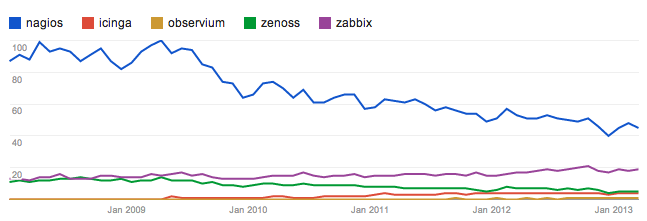
\includegraphics[scale=0.6]{img/monitoring_google_trends}
    \caption{Google Trends: overvåkningsløsninger}
    \label{losninger}
\end{figure}

\section{Valg av kjerneprogramvare}
Valg av kjerneprogramvare var gruppens viktigste valg, da det la grunnmuren for resten av prosjektet, og ville få stor innvirkning på sluttresultatet. Av kandidatene nevnt i \ref{sec:hvilkefinnes}, ble Icinga og Nagios videre vurdert.  

Icingas distribuerte system består av kjernen, som står for prossessering, et databaselag, og administrering av systemet via et webgrensesnitt. Dette er tilrettelagt for et distribuert oppsett. Nagios sin arkitektur har avhengigheter mellom web og lagring av status, som fører til at disse ikke kan separeres. Det er derimot mulig å separere ut MySQL-databasen som Nagios benytter\cite{icingaarchitecture}.

For uthenting av informasjon i Icinga er det utviklet et API som brukes via Icinga Web. Dette gir ett punkt for uthenting av data, med samme oppbygging for alle spørringer. I Nagios er det ikke noen standardisert måte å hente ut informasjon\cite{icingaapi}.

En annen fordel med Icinga er støtte for LDAP-autentisering i Icinga Web, som videre kan benyttes til å styre tilgang til ulik informasjon for brukere. Med Nagios kan en også innføre LDAP-støtte, men dette blir da autentisering via en web-server, og videre kontroll av aksess er ikke mulig. Nagios har noe aksesstyring, men det er bare på et objekt kalt ``contactgroups''. Icinga har aksesstyring på en rekke flere objekter\cite{icingaweb}.

For databaseoppsett støtter Icinga de tre databasemotorene PostgreSQL, Oracle og MySQL. Nagios har bare støtte for MySQL. I oppgavebeskrivelsen er det krav om MySQL, men for fremtidig bruk av Icinga er det mulighet for å benytte de to andre.

Icinga har også en tilleggsmodul kalt ``Icinga Mobile''. Denne gir tilrettelagt grensesnitt for mobile enheter, som var ønsket i oppgavebeskrivelsen. Icinga Mobile kan brukes for å gi et grensesnitt tilpasset mindre skjermer. Ved utsendelse av SMS eller e-post til en eller flere ansatte, kan Icinga-Mobile brukes via samme enhet for å se mer utfyllende informasjon om problemet, samt gjøre administrative handlinger.

Etter en vurdering av denne funksjonaliteten, ble det besluttet å basere overvåkningsløsningen på Icinga framfor Nagios.
\clearpage
\section{Icinga}
For å kunne forstå implementasjonsdelen av prosjektrapporten er det behov for noe innsikt i hvordan Icinga fungerer. I dette delkapittelet er det viktigste forklart.
\subsubsection{Arkitektur}
Icinga består av tre separate komponenter, som vist i Figur \ref{icingacomponents}.

\begin{figure}[H]
    \centering
    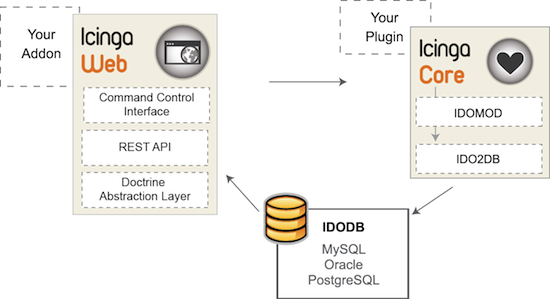
\includegraphics[scale=1.2]{img/icinga_architecture}
    \caption{Icingas tre komponenter}
    \label{icingacomponents}
\end{figure}

\subsubsection{Core}
Icinga Core håndterer planlegging av sjekker gjennom plugin-er og tar i mot resultatene av disse. Denne informasjonen sendes gjennom SSL-krypterte TCP-sockets videre til IDO2DB-prosessen (Icinga Data Out to Database) gjennom et interface kalt IDOMOD (Icinga Data Out Module). Ved å bruke disse abstraksjonslagene kan databasemotoren enkelt byttes ut. I dokumentasjonen er det laget veiledninger for MySQL, PostgreSQL og Oracle\cite{icingaarchitecture}.

IDOMOD og IDO2DB kommer i en samlet pakke (IDOutils), men kan separeres ut for å skape et distribuert oppsett. CERN i Sveits har nylig implementert et slikt oppsett med hjelp av lastbalansereren ``Mod Gearman''\cite{cernthesis}.

\subsubsection{Web}\label{sec:teoriweb}
I utgangspunktet kommer ikke Icinga med noe webgrensesnitt. Men det er mulig å installere to forskjellige pakker for å få dette. I begge kan en få en oversikt over tilstanden til enheter og tjenester, se konfigurasjon og utsendte varsler, samt utføre administrative oppgaver. Det kan også hentes ut statistikk over oppe- og nedetid.

Icinga Classic baserer seg på det samme vindusoppsettet som Nagios. For uthenting av data benyttes CGI-moduler som henter ut data fra filen ''status.dat''. Filen blir brukt av Icinga for å lagre tilstandsinformasjon om enheter og tjenester, kommentarer, og informasjon om nedetid. 

Icinga Web er en total omskrivning av webgrensesnittet. Det er en Ajax-drevet, Web 2.0-inspirert front-end, som har flere lag mellom kjernen av Icinga og visningene:

\textbf{Doctrine Abstraction Layer} henter informasjon fra databasen. Det kan også benyttes av utviklere for å legge til egne moduler i Icinga Web med uthenting av informasjon fra andre databaser.
\textbf{REST API} presenterer dataene fra DAL til Icinga Web. Her kan autentisering utføres slik at en kan sette hvilken informasjon ulike brukere skal kunne se.
\textbf{Command Control Interface} kan videresende kommandoer til Icinga Core. For eksempel manuell kjøring av en sjekk eller restart av Icinga. 

\section{Objekter}\label{sec:objekter}
All konfigurasjon av Icinga gjøres i tekstfiler. I selve konfigurasjonsfilen ''icinga.cfg'' settes filbanen til konfigurasjonsfilene. Icinga vil da ved oppstart lete rekursivt gjennom mappen etter filer som ender med ''.cfg''.

Konfigurasjonsdataene er bygget rundt det som i Icinga kalles objekter. Dette er en samling av konfigurasjon som hører sammen. Selv om en ikke kan si at Icingas objekter er det samme som objekter i programmeringsverden, benyttes mange av de samme begrepene og konseptene.

En rekke objekter er definert i Icinga, som vist i Tabell \ref{objekter}.

\begin{changemargin}{-1cm}{-1cm}
\begin{table}
\begin{center}
%\begin{tabular}{|p{2.0in}|c|c|c|} \hline
\begin{tabular}{ | p{3.5cm} | p{6.5cm} | p{6cm} |} \hline
	\textbf{Objekt} & \textbf{Forklaring} & \textbf{Eksempel} \\ \hline
	Host & En enhet med en adresse (typisk IP-adresse eller MAC-adresse). & Server, switch, router etc. \\ \hline
	Command & En kommando som skal kjøres på overvåkningsserveren & Et program, for eksempel check\_ping. \\ \hline 
	Service & Kombinasjonen av et host-objekt og et command-ojekt. & Sjekk oppetid: kommandoen ``check\_uptime'' skal kjøres på ``dc1''. \\ \hline
	Servicegroup & Service-objekt knyttet til host-objekter satt sammen til en applikasjon. & En applikasjon har tre prosesser som må være kjørende for at applikasjonen fungerer. Disse grupperes under samme servicegroup. \\ \hline
	Contact & Når og hvordan en person skal kontaktes angående en service. & Jens skal få en SMS hvis DHCP ikke er tilgjengelig. \\ \hline
	Timeperiod & Navn og definisjon av en tidsperiode. & Mellom 08.00 og 16.00 på annenhver tirsdag, hvis det er den tredje dagen i måneden. \\ \hline
	Host dependency & En eller flere avhengigheter. Dersom et host-objekt er avhengig av et annet, og det ikke svarer lenger, trenger ikke Icinga utføre sjekker på det avhengige objektet. & kantswitch1 er avhengig av kjerneswitch. \\ \hline
	Service dependency & Samme som host, men for service. & Captive portal er avhengig av RADIUS. \\ \hline
	Host escalation & Hva skal skje etter at en host har vært nede etter en definert tid. &	Om dc1 har vært nede i 30 minutter, send e-post til Ola Sysadmin. Etter 60 minutter sendes SMS til alle i admin contactgroup-en \\ \hline
	Service escalation & Samme som for objektet host-dependency, men for service-objeker. & Om DNS har vært nede i 30 minutter, send e-post til Kari Sysadmin. Etter 60 minutter send SMS til alle i admin hostgroup-en. \\ \hline
	\end{tabular}
	\caption{Oversikt over objekter i Icinga}
	\label{objekter}
\end{center}
\end{table}
\end{changemargin}

I tillegg til disse kan host, service og contact grupperes med henholdsvis hostgroup, servicegroup og contactgroup.

Det er også to objekter med metainformasjon, ``hostextinfo'' og ``serviceextinfo'', der en kan definere ekstra konfigurasjon som bildebaner, notater og koordinater for host- og service-objekter.

Den siste objekttypen er module. Her spesifiseres konfigurasjon for en modul som utvider funksjonalitet i Icinga Web.

Sammenhengen mellom objektene er viktig å forstå for å skjønne hvordan sjekker utføres i Icinga. I et service-objekt defineres hvilket command-objekt som skal benyttes for å teste tjenesten og hvilke host- eller hostgroup-objekter dette skal sjekkes på. Dette er vist i Figur \ref{command_host_service}.

\begin{figure}[H]
    \centering
    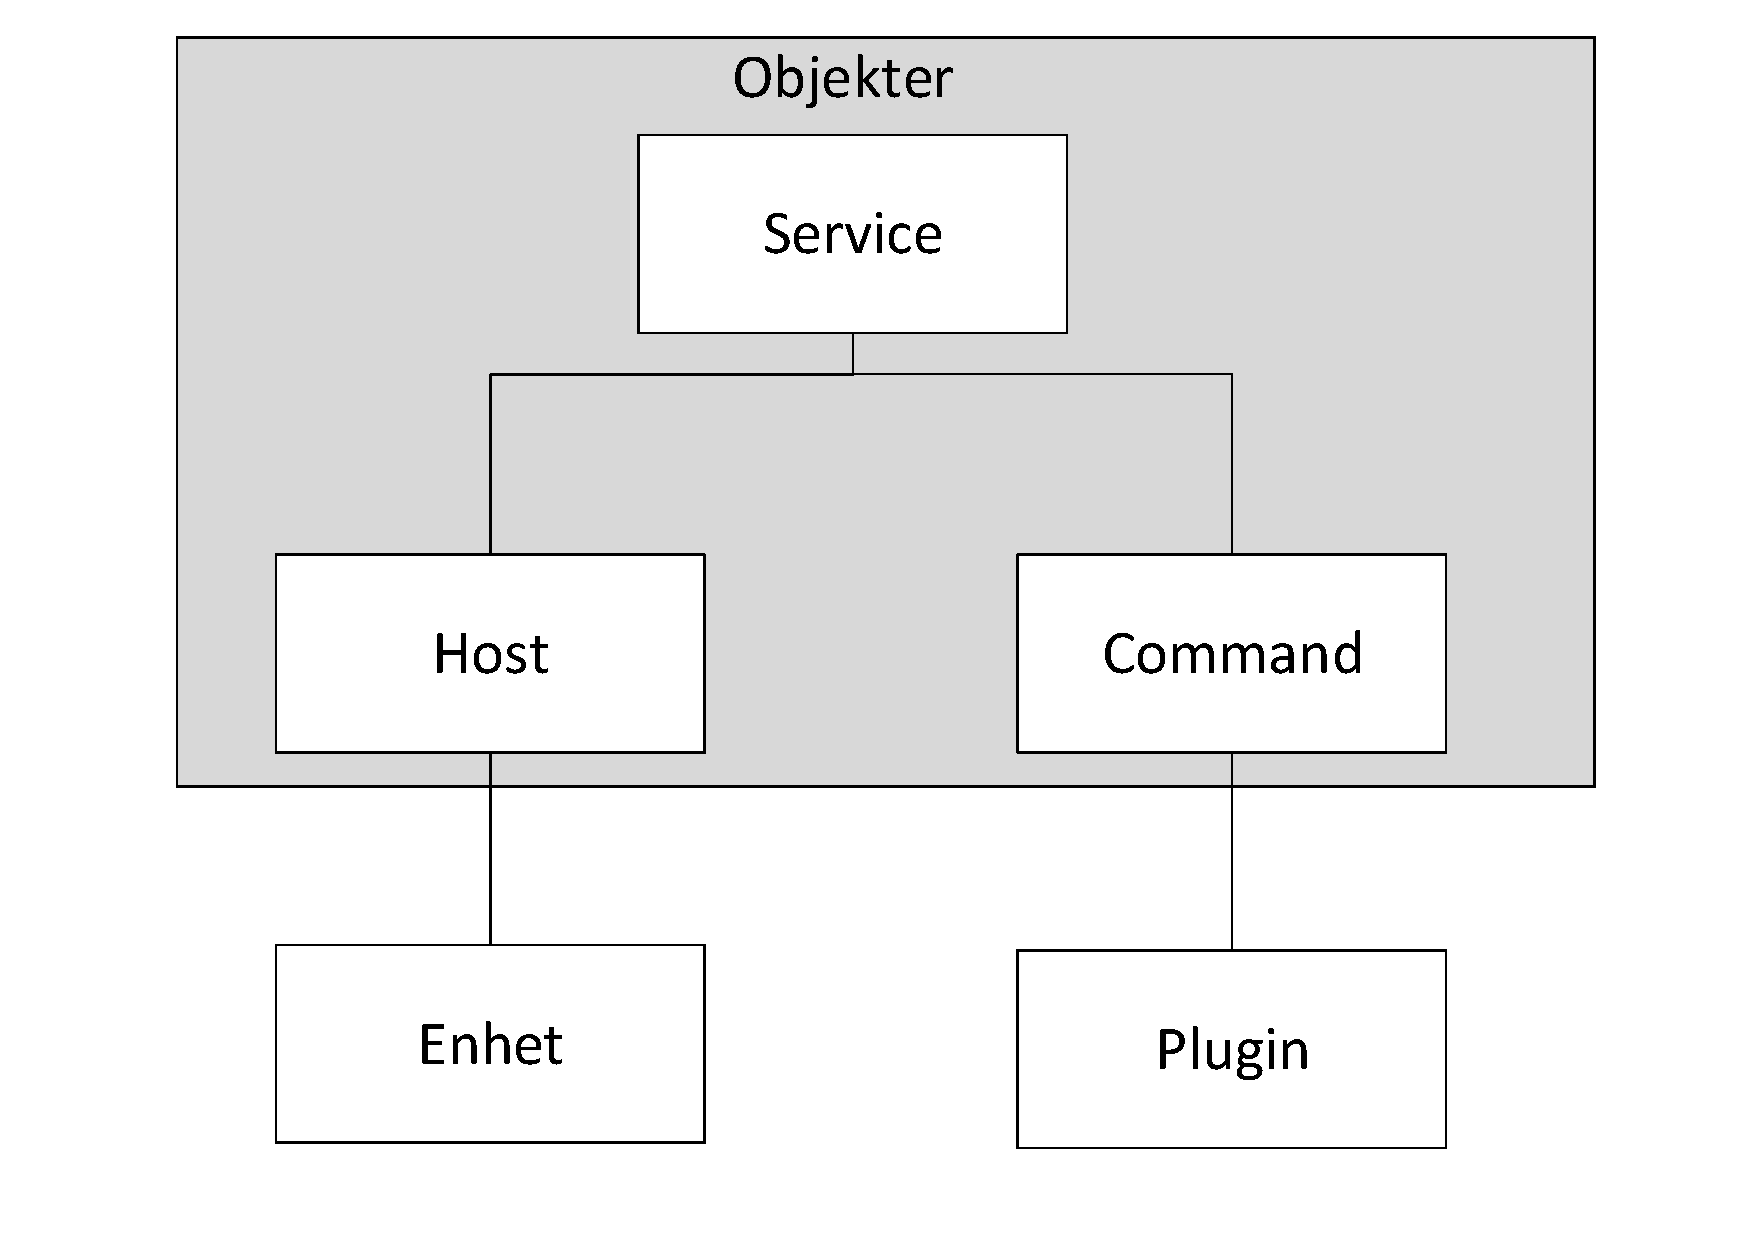
\includegraphics[scale=0.4]{img/command_host_service}
    \caption{Sammenhengen mellom host-, service- og command-objekter.}
    \label{command_host_service}
\end{figure}
% Si noe om utelatt konfig, arv ved use?
I eksempelet under vises konfigurasjonen for å sette opp en ping-sjekk på HiG1.
\begin{lstlisting} [style=example]
define host {
    use                  generic_host
    host_name            HiG1
    address              192.168.0.1
}

define service {
    use	                 generic_service
    host_name            HiG1
    service_description  Ping
    check_command        check_ping!200,5%!500,10%
    check_interval       5
}

define command {
    command_name         check_ping
    command_line         /usr/lib/nagios/plugins/check_ping -H $HOSTADDRESS$ --warning $ARG1$ --critical $ARG2$   
}
\end{lstlisting}

\clearpage
\section{Plugin-er}
Icinga i seg selv kommer uten noen overvåkningssjekker. Til dette benyttes plugin-er.

En plugin i Icinga er et eksternt program som kjøres og outputen hentes inn som data. Resultatet av sjekken hentes fra exit-koden\cite{wiki:returncode} og oversettes til en tilstand, som vist i Tabell \ref{state}.

En plugin kan være noe helt enkelt som scriptet under. Der exit-koden til en ping-kommando sjekkes. Hvis ping ikke får svar, vil den gi exit-koden 1. Scriptet vil da gi exit koden 2, som i Icinga oversettes til CRITICAL.
\begin{lstlisting}[language=bash]
#!/usr/bin/env bash
loss=$(ping -c 5 google.com)
if [ $? -eq 0 ]; then
    echo "OK"
    exit 0
else
    echo "ERROR"
    exit 2
fi
\end{lstlisting}

Det finnes et sett med offisielle plugin-er til Nagios; nagios-plugins, som utgis av ``Nagios Plugins project''. Pakken finnes i en rekke pakkebehandlere og inneholder over 50 plugin-er som er ment for å dekke et grunnleggende overvåkningsbehov\cite{nagiosplugins}.

\begin{table}[H]
	\begin{center}
	\begin{threeparttable}
	\begin{tabular}{| l | l | l |} \hline
	\textbf{Returkode fra plugin} & \textbf{Service-tilstand} & \textbf{Host-tilstand} \\ \hline
	0 & OK & UP \\ \hline
	1 & WARNING & UP eller DOWN/UNREACHABLE* \\ \hline
	2 & CRITICAL & DOWN/UNREACHABLE \\ \hline
	3 & UNKNOWN & DOWN/UNREACHABLE \\ \hline
	\end{tabular}
	\begin{tablenotes}
	\small
	\item *Ved bruk av Aggressive host checking\cite{icingapluginapi}.
	\end{tablenotes}
	\caption{Tilstandsoversikt}
	\label{state}
	\end{threeparttable}
	\end{center}
\end{table}

\section{Sjekker}\label{sec:sjekker}
Tilstanden for et service- eller host-objekt vil bestemmes ut i fra et returnert resultat fra en aktiv eller passiv sjekk. Forskjellen på disse to vil bli forklart i de neste delkapitlene.

Dersom en aktiv eller passiv sjekk resulterer i en annen tilstand enn OK, er det to typer av tilstanden, ``SOFT'' og ``HARD''. Første gang en plugin returnerer en feil vil tilstanden bli satt til SOFT, i tillegg til service- eller host-tilstanden. Etter dette vil sjekken kjøres hyppigere for å finne ut om det er snakk om et forbigående problem. Etter et gitt antall ganger der plugin-en fortsatt ikke returnerer OK, vil tilstanden skifte til HARD og det sendes ut varslingsmelding. Varsling er beskrevet grundigere i \ref{sec:varsling}.

\clearpage
\subsubsection{Aktive sjekker}
En aktiv sjekk er en sjekk som initieres av Icinga, der en kommando kjøres på Icinga-serveren. Dette er også kjent som en ``poll''-modell. En aktiv sjekk defineres ut i fra et command-objekt med parametere og et tidsintervall i service- og host-objekter. I command-objektet defineres en plugin som skal kjøre, og returverdien fra denne vil bestemme hvilken tilstand service- eller host-objektet har. I Figur \ref{active_checks} vises komponentene involvert i en aktiv sjekk.
\begin{figure}
   \centering 
   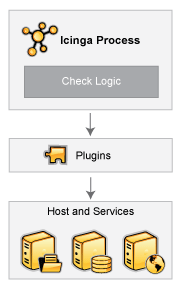
\includegraphics[scale=0.7]{img/activechecks.png}
    \caption{Aktive Sjekker}
    \label{active_checks}
\end{figure}

\subsubsection{Passive sjekker}
Passive sjekker går motsatt vei av aktive sjekker. Her vil hver host si ifra når verdier har overgått en satt grense eller en feil har oppstått. Dette kalles ofte for en ``push''-modell. Passive sjekker kjøres ved at et eksternt program skriver en linje med informasjon om tjenesten og sjekkresultat til en fil, som Icinga sjekker periodisk. Dette er illustrert i Figur \ref{passive_checks}.

Fordelen med passive sjekker er at Icinga vil oppdage feil raskere. Ved standard konfigurasjon sjekkes filen med sjekkresultater så ofte som mulig, mens aktive sjekker kjøres hver 5. minutt. Passive sjekker vil også avlaste Icinga-serveren, da alle sjekker utelukkende vil bli kjørt lokalt på enheten som overvåkes. Men en må åpne for at kommunikasjon kan initieres fra alle enheter som skal overvåkes til Icinga-serveren, og mister da samtidig muligheten til å samle all konfigurasjon på ett sentralt sted. 

\begin{figure}[H]
    \centering
    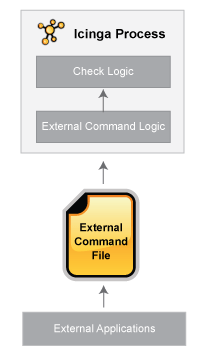
\includegraphics[scale=0.7]{img/passivechecks.png}
    \caption{Passive Sjekker}
    \label{passive_checks}
\end{figure}

\subsubsection{Hostsjekk}
Resultatet av en host-sjekk vil avgjøre om tilstanden til host-objektet er ``UP'' eller ``DOWN''. 

Det er ikke et fast tidsintervall for en hostsjekk med mindre check\_interval er definert for objektet. Icinga vil kjøre sjekken om en service som er satt opp for host-en skifter tilstand. Service-objekter som er definert for en host som er i ``DOWN'' vil automatisk bli vist under ``Known service problems'' i webgrensesnittet, og ingen sjekker vil bli kjørt på dem før host-en er ``OK'' igjen.

Grunnsjekken for en host defineres i host-konfigurasjonen med ''check\_command'', som vist under.
\begin{lstlisting}[style=example]
define host {
...
    check_command	check_host_alive
}
\end{lstlisting}

\subsubsection{Variabler}
For å kunne gjøre konfigurasjon av Icinga mest mulig dynamisk er det en rekke forhåndsdefinerte variabler en kan bruke i konfigurasjonsfilene. Disse kalles makroer. En fullstendig liste over disse og hvor de kan benyttes finnes i Icinga-dokumentasjonen\cite{icingamacro}. ''\$HOSTADDRESS\$'' kan for eksempel benyttes i et command-objekt slik at det bare må skrives en gang, og ikke for hver host. En kan også definere egne variabler som for eksempel ''\_SSHPORT''. Disse kan sendes videre til selve kommandoen som kjøres og benyttes som argumenter til plugin-en som kjører en sjekk, slik:
\begin{lstlisting}[style=example]
define host {
...
    host_name		example_server
    _SSHPORT		222
}
define command {
    command_name	check_ssh
    command_line	$USER1$/check_ssh -H $HOSTADDRESS$ -p $_HOSTSSHPORT$
}
\end{lstlisting}

Her benyttes de innebygde variablene ``USER1'' for banen til plugin-en som kjøres, HOSTADDRESS for IP-en til den hosten som sjekken skal kjøres på og den egendefinerte variabelen \_SSHPORT som defineres på host-objektet.

USER-variablene defineres i den globale konfigurasjonsfilen og brukes der hvor informasjon skal sjules fra webgrensesnittet. Som for eksempel når det trengs et passord for å utføre en sjekk.

\subsubsection{Templates}
En template er ikke et objekt i seg selv, men en mal for et objekt. Med direktivet ``register 0'' vil ikke Icinga registrere dette objektet for overvåkning. Ved å bruke direktivet ``use'' kan en i et annet objekt ``arve'' konfigurasjonen fra template-en. Template-er kan også arve, og en kan dermed sette opp et hierarki der en spesifiserer generell konfigurasjon i toppen og arver nedover til mer spesiell. 

I eksempelet under er generell konfigurasjon for alle host-objekter definert i ``generic\_host'', som brukes i de andre objektene. I ``generic\_firewall'' erstattes verdien for kontaktgruppe, og i cisco\_firewall settes en egendefinert variabel:

Template-en generic\_host: 
\begin{lstlisting}[style=example]
define host {
    name                            generic_host    ; The name of this host template
    notifications_enabled           1       ; Host notifications are enabled
    event_handler_enabled           1       ; Host event handler is enabled
    flap_detection_enabled          1       ; Flap detection is enabled
    failure_prediction_enabled      1       ; Failure prediction is enabled
    process_perf_data               1       ; Process performance data
    retain_status_information       1       ; Keep status after Icinga restart
    retain_nonstatus_information    1       ; Keep non-status after Icinga restart
    check_command                   check-host-alive
    max_check_attempts              10
    normal_check_interval           5
    retry_check_interval            2
    notification_interval           0
    notification_period             24x7
    notification_options            d,u,r
    contact_groups                  all_contacts
    register                        0       ; Not a real host, just a template
}
\end{lstlisting}

Template-en generic\_firewall, som arver fra generic\_host:
\begin{lstlisting}[style=example]
define host {
   name             generic_firewall
   use              generic_host
   contact_groups   firewall_admins
   register         0
}
\end{lstlisting}

Template-en cisco\_firewall, som arver fra generic\_firewall:
\begin{lstlisting}[style=example]
define host {
    name            cisco_firewall
    use             generic_firewall
    register        0
    _WANPORT        WAN ; Custom variable for WAN port to monitor
}
\end{lstlisting}

Host-objektet hig-hw1, som arver fra cisco\_firewall:
\begin{lstlisting}[style=example]
define host {
    use             cisco_firewall
    host_name	    hig-fw1
}
\end{lstlisting}

Dette gjør at det blir lite konfigurasjon hver gang en ny brannmur skal legges til.

\subsubsection{Regulære uttrykk}
Ved å sette ``use regular expressions'' i konfigurasjonen for Icinga, kan en benytte regulære uttrykk i attributter i et objekt, der en refererer til andre objekter. Icinga støtter standarden POSIX Extended Regular Expressions, og vil automatisk tolke navnet på objekter som et regulært uttrykk dersom det inneholder \verb|"*", "?", "+", eller "\"|.

Dette kan være nyttig dersom en for eksempel vil legge alle hoster i en hostgroup, som har en navnekonvensjon som gjør at hver av hostene unikt kan identifiseres ved å bytte ut deler av navnet med en variabel.

I eksempelet nedenfor brukes det regulære uttrykket \verb|"^HiG\[0-9\]+\$"| i attributten ``members'' til å legge til alle konfigurerte hosts der navnet starter på ``HiG'' etterfulgt og avsluttet med ett eller flere siffer mellom 0 og 9, i hostgroup-objektet ``all\_servers''.
\begin{lstlisting}[style=example]
define hostgroup {
    hostgroup_name	all_servers
    alias		All Servers
    members		^HiG[0-9]+$
}
\end{lstlisting}

Det kan også benyttes til å ekskludere en host fra en service-sjekk. I eksempelet nedenfor er HiG3 medlem av hostgroup-en ``windows\_servers'', men blir ekskludert fra å kjøre sjekken på diskplass ved å sette ``!HiG3'':
\begin{lstlisting}[style=example]
define service {
    use				generic_service
    service_description		Disk space
    hostgroup_name		windows_servers
    host_name			!HiG3
    check_command		win_nrpe!CheckDriveSize!Drive="C" MaxWarnUsed=80% MaxCritUsed=90%
}
\end{lstlisting}

\section{Avhengigheter}
I Icinga kan en definere tre ulike typer avhengigheter, ``Parent'', ``Service dependency'', og ``Host dependency''. Disse har innvirkning på hvilke varsler som sendes ut og statusen de ulike service- og host-objektene får. Hver av disse krever egen konfigurasjon. 

\section{Parent}\label{sec:parent}
Et host-objekt kan settes som en parent til et annet host-objekt. Host-objekter som har en parent blir betegnet som en child-host eller child-service. Dette brukes primært for å unngå varsler om andre host- og service-objekter enn det som er definert som parent, om denne blir utilgjengelig. For eksempel hvis kjernerouteren mister strømtilgangen, ønskes ikke varsler for eventuelle host-objekter og tilhørende service-objekter som har kjernerouteren som parent. Disse vil ikke lenger bli sjekket og tilstanden vil bli satt til ``UNREACHABLE''. Tjenester som tilhører host-ene vil få tilstanden ``UNKNOWN''.

For redundante oppsett kan et host-objekt ha flere ``parents'' definert. Host-objektet vil da ha tilstanden UP så lenge minst én ``parent''-host er UP.

Ut ifra parent-relasjonene mellom host-objekter i konfigurasjonsfilene genereres også et ``Status Map'' over nettverket, som vist i Figur \ref{statusmap}. Dette brukes til å visualisere alle relasjonene, og vil gjengi redundante oppsett og hvilke host-objekter som er påvirket av at parent-hosten er DOWN.

\begin{figure}[H]
    \centering
    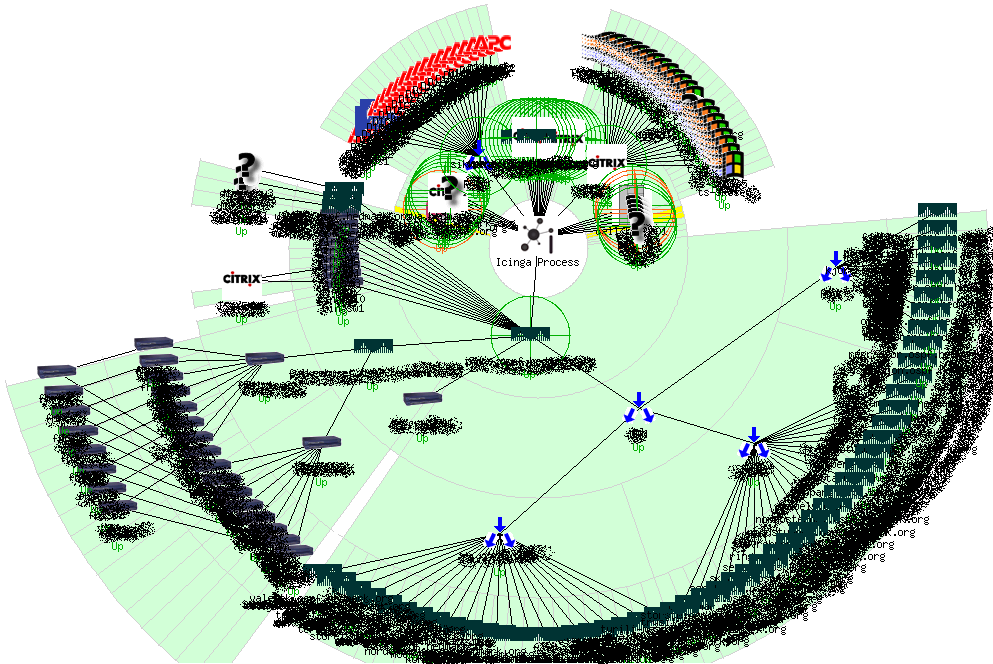
\includegraphics[scale=0.6]{img/statusmap}
    \caption{Kart som viser parent- og host-relasjoner}
    \label{statusmap}
\end{figure}

\section{Service dependency}\label{sec:servicedependency}
Service dependency er en egen objekttype der en kan sette opp avhengighet mellom to service-objekter. Formålet med dette er å unngå varsel hvis en tjeneste får tilstanden DOWN, som følge av at en annen tjeneste har det. For eksempel bør det ikke varsles om at tjenester som er avhengig av autentisering via LDAP-serveren får ``Access Denied''-feilmeldinger, hvis LDAP-serveren er DOWN. Det service-objektet andre service-objekter er avhengige av kalles en master service. 

Icinga undersøker om avhengigheter er definert for et service-objekt, før det utføres sjekker på det. Dette er med på å bestemme om det blir sendt ut varsel for service-objektet.

I eksempelet under er tjenesten ``Check SMB'' på HiG3 avhengig av master-service-en Check LDAP på HiG3. ``execution\_failure\_criteria'' bestemmer ved hvilke tilfeller tjenesten ikke skal sjekkes. Her er den satt til ``c'', som vil si at Check SMB ikke skal kjøres dersom ``Check LDAP'' er i CRITICAL tilstand.

\begin{lstlisting}[style=example]
define servicedependency {
    host_name                          HiG3
    service_description                Check LDAP
    dependent_host_name                HiG3
    dependent_service_description      Check SMB
    execution_failure_criteria         c
    notification_failure_criteria      c
}
\end{lstlisting}

Ved standard konfigurasjon vil Icinga benytte siste harde tilstand for master service. Dersom ``max\_check\_attempts'' for eksempel er satt til 4, vil ikke Check SMB stoppes fra å kjøres før Check LDAP har blitt sjekket fire ganger, og oppnår en hard tilstand. 

På attributten notification\_failure\_criteria kan det settes hvilke service-tilstander en ikke skal varsle for. Dette er hovedgrunnen til at det settes opp slike avhengigheter. Når denne er satt til ``c'' vil det ikke varsles om master service-en får tilstanded CRITICAL.

Service-objekter har kan også arve avhengighetene til en master service ved å sette direktivet ``inherits\_parent 1''. For eksempelet over vil Check SMB da arve fra service-objekter som Check LDAP arver fra.

For å konfigurere avhengigheter mellom tjenester som kjører på samme host kan en utelate ``dependent\_host\_name'' I eksempelet under vil alle tjenester på host-objektet være avhengig av tjenesten ``NRPE-daemon''.

\begin{lstlisting}[style=example]
define servicedependency{
    ;dependent_host_name   	    ; Not defined to make dependancy on same host            
    hostgroup_name 		    linux_servers
    service_description             NRPE-daemon
    dependent_service_description   NRPE Check *
    execution_failure_criteria      c
    notification_failure_criteria   c
}
\end{lstlisting}

En kan også erstatte host\_name og dependant\_host\_name med hostgroup og dependant\_host\_group for å lage avhengigheter på alle objekter som tilhører gruppen.

\section{Host dependency}
For å sette en avhengighet mellom to host-objekter benyttes host dependency. Dette må ikke forveksles med parent, som refererer til nettverksoppsettet. En host dependency vil si at et host-objekt er avhengig av et annet host-objekt. Host dependency er bare nyttig i veldig spesielle tilfeller, da det for de fleste tilfeller vil være avhengigheter til en eller flere tjenester på host-en\cite{hostandservicedep}, eller at en host er avhengig av å kjøre en sjekk igjennom en annen host.

\section{Protokoller og agenter}
For å kjøre sjekker på enheter må Icinga-serveren kunne kommunisere med operativsystemene på de ulike enhetene. Icinga henviser til protokollene SSH, SNMP, RPC (WMI) og agentene NRPE og NSCA (en del av pakken NSClient++) i dokumentasjonen\cite{icingaintegration,icingaadditionalsoftware}. 

\subsubsection{NRPE}\label{sec:nrpe}
NRPE (Nagios Remote Plugin Executor) består av plugin-en ``check\_nrpe'' på Icinga-serveren og en daemon som installeres på hver server som skal overvåkes. NRPE eksekverer lokale plugin-er på den eksterne serveren og returner dataen fra denne til check\_nrpe. Tillatelse for eksekveringer defineres i en konfigurasjonsfil på hver server, der en oppgir hvilke IP-adresser som kan koble seg til og hvilke kommandoer som er gyldige. 

\begin{figure}[H]
    \centering
    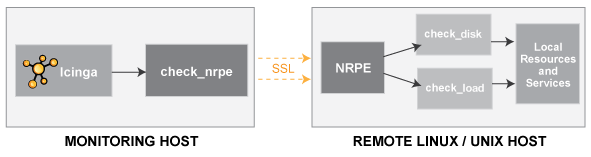
\includegraphics[scale=0.6]{img/nrpe.png}
    \caption{NRPE}
    \label{nrpe}
\end{figure}

\subsubsection{SSH}
Gjennom en tilkobling til en SSH (Secure Shell)-server kan en spesifisere en kommando som skal kjøres på en ekstern maskin, og hente output-en til det opprinnelige shellet. Dette virket som den beste måten å overvåke Linux-servere på, ved starten av prosjektet. SSH-prosjektet er meget utbredt og blir aktivt sjekket for sikkerhetshull. SSH er også installert på de aller fleste Linux-servere, og en vil dermed unngå å lytte på en ekstra port.

Ulempen med å kjøre sjekker over SSH er at en må sette opp nøkkelbasert innlogging mellom Icinga-serveren og alle Linux-serverne som skal overvåkes. En kan begrense rettigheter for brukeren som kjører sjekkene, men den vil fortsatt ha muligheten til å logge inn til et shell og eksekvere kommandoer. Dette kan føre til at en potensiell angriper via Icinga-serveren, har en vei inn til alle servere som overvåkes, ved å bruke den private nøkkelen.

SSH gir også endel overhead både på nettverkstrafikk og i CPU-tid\cite{sshmanpage}. En måte å begrense dette på er å benytte SSH med ControlMaster. Dette innebærer en endring i SSH-konfigurasjonen på serveren, slik at SSH-klienten lagrer informasjon om hver utgående TCP-tilkobling, og samme tilkobling kan benyttes mot samme host. Dermed unngås en ny TCP-tilkobling for hver ny sjekk som skal utføres på hosten.

\subsubsection{SNMP}
Det meste av nettverksutstyr beregnet for bedrifter, har i dag støtte for protokollen SNMP (Simple Network Management Protocol\cite{essentialsnmp}). SNMP definerer en enkel og effektiv måte å overvåke enheter på og det gir en standard som leverandørene følger.
	
SNMP baserer seg på variabler som blir gjort tilgjengelig på enheten som skal overvåkes (kalt agenten). Disse variablene er definert i en Management Information Base (MIB). MIB-filene er ofte tilgjengelige på produsentens hjemmeside. Her beskrives strukturen for dataen i et hierarkisk navnerom som inneholder Object Identifier (OID). Hver OID identifiserer en variabel som kan bli lest eller satt via SNMP. Enheten som ber om disse variablene kalles ``manager''. 

En ulempe med SNMP er at OID-ene er lange og tunge å lese. For eksempel for å hente ut batterikapasiteten på en APC UPS benyttes OID-en:
\
1.3.6.1.4.1.318.1.1.1.2.2.1.0
\
Dette kan oversettes til:
\
iso(1). org(3). dod(6). internet(1). private(4). enterprises(1). apc(318). products(1). hardware(1). ups(1). upsBattery(2). upsAdvBattery(2) upsAdvBatteryCapacity.0
\
Denne OID-en er definert i APCs MIB-fil ``PowerNet MIB''. Ved å laste inn denne kan en også benytte ``PowerNet-MIB::upsAdvBatteryCapacity.0''.

SNMP finnes i flere versjoner. I dag brukes for det meste versjon 2c og den nyeste, versjon 3. De ulike versjonene er ikke kompatible, men i praksis støtter det meste av utstyr som støtter v3 eller v2c også v1 \cite{rfc3584}. Hovedforskjellen på versjon 2c og 3 er at versjon 3 har støtte for flere sikkerhetsmekanismer, men krever noe mer konfigurasjon. Sikkerhetsaspektet ved dette er diskutert videre i Kapittel \ref{chap:sikkerhet}.

Det eksisterer to muligheter når enheter skal overvåkes via SNMP. Enten kan enhetene selv rapportere inn hendelelser via SNMP trap/inform, eller så kan serveren spørre enhetene via SNMP GetRequest. Valg av det første medfører at en kan gjøre varsling umiddelbart, men da må også hver enhet konfigureres med parametere for hvilke trap-meldinger som skal sendes og til hvilken IP-adresse. Icinga har ingen støtte for å motta trap-er, men en kan installere en egen daemon for dette og rapportere inn data med passive sjekker. 

For å benytte SNMP trap/inform må en tillate tilkoblinger til overvåkingsserveren i stedet for bare fra denne. Hvilke trap-meldinger som skal sendes må også konfigureres på hver enhet, og en vil da ikke kunne ha alle konfigurasjoner sentralisert på Icinga-serveren.

\begin{figure}[H]
    \centering
    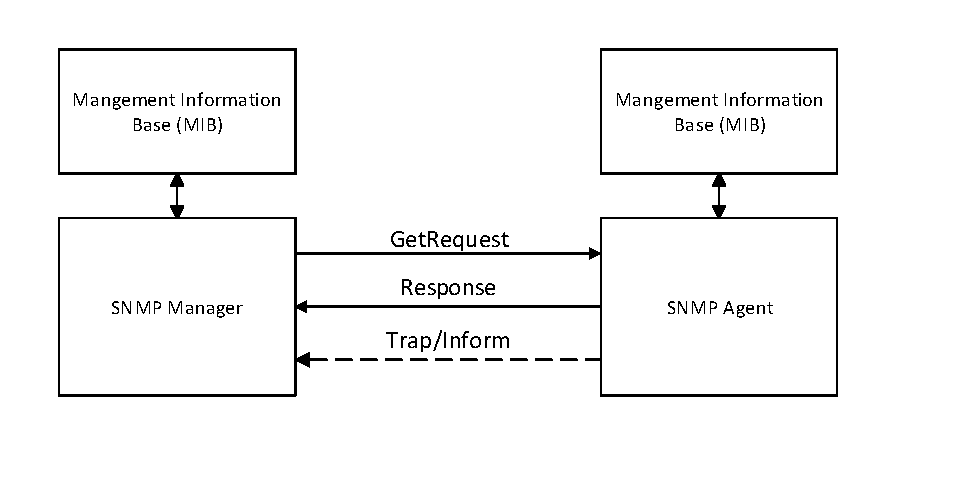
\includegraphics{img/SNMP}
    \caption{Overvåkning med SNMP}
    \label{SNMP}
\end{figure}

SNMP benytter seg av UDP for å levere trap-meldinger. UDP er en såkalt upålitelig protokoll, noe som vil si at det ikke er noen omsending av pakker eller noen tilbakemelding (ack) for at pakkene kommer fram. Derfor kan en risikere å miste en trap. SNMP inform, som kom i SNMPv3, løser dette ved at agenten vil sende en ny inform-pakke i et intervall, helt til manageren gir beskjed om at trap-meldingen er mottatt.

For å benytte SNMP på Windows- og Linux-servere kreves installasjon av en SNMP-agent\cite{mssnmp,netsnmp}.

\subsubsection{WMI (Windows Management Instrumentation)}
WMI er et grensesnitt som gjør det mulig å lage programmer eller script som utfører oppgaver mot operativsystemet Windows, både lokalt eller på eksterne maskiner. Disse oppgavene kan være alt fra å restarte maskinen, til å hente ut logger over hendelser som har inntruffet på maskinen. I en overvåkningsløsning vil det være mest relevant å kjøre kommandoer som henter ut informasjon om maskinen og tjenester som kjører på den. Dette kan for eksempel være hvilke prosesser som bruker mest CPU-tid.

For å benytte WMI-spørringer direkte fra en ekstern enhet må det konfigureres brukertilgang og brannmurregler\cite{wmiremote}. Med NSclient++ har en mulighet til å kjøre WMI-spørringer over NRPE uten ekstra konfigurasjon.

\subsubsection{Valg av Agenter}
Valg av protokoll eller agenter har basert seg på følgende punkter:
\begin{itemize*}
	\item Ressursbruk (CPU)
	\item Nettverkstrafikk
	\item Utrulling
	\item Sikkerhet
\end{itemize*}
Nettverkstrafikken som ble generert ved både en NRPE- og en SSH-sjekk ble målt ved å benytte et Bash-script som kjørte en disk-sjekk 100 ganger, som vist under. 

\begin{lstlisting}[style=example,language=bash]
#!/usr/bin/env bash
if [ "$1" == "ssh" ]; then
    cmd="/usr/lib/nagios/plugins/check_by_ssh -H 10.60.0.21 -C \"/usr/lib/nagios/plugins/check_disk -W 10% -C 5% -M -A\" > /dev/null"
elif [ "$1" == "nrpe" ]; then
    cmd="/usr/lib/nagios/plugins/check_nrpe -H 10.60.0.21 -c check_all_mounts -a 10,5 > /dev/null"
else
    echo "You must specify ssh or nrpe as the first argument"
    exit 1
fi
for i in {1..100}; do
    eval $cmd
done
exit 0
\end{lstlisting}

Både serveren og klienten stod i et eget nettverk i Virtualbox sammen med en Windows-maskin med et nettverkskort satt i promiscious mode, for å kunne sniffe nettverkstrafikken. Denne fanget nettverkstrafikken med Wireshark. Trafikken mellom de to maskinene ble hentet ut og data for hver tilkobling ble brukt til å kalkulere båndbreddebruk.

Det ble også undersøkt hvor mye CPU-tid NRPE og SSH trenger for å utføre sjekker. Fordi hver sjekk går veldig raskt ble det kjørt 100 disksjekker, 100 ganger. ``time''-kommandoen ble brukt for å se på tiden brukt i user- og kernel-mode. Dette ble gjort ved å bruke Bash-scriptet nedenfor, som kjører det samme scriptet som ble brukt for å generere nettverkstrafikk.

\begin{lstlisting}[style=example]
#!/usr/bin/env bash

args=(nrpe ssh)

for arg in "${args[@]}"; do
        for i in {1..100}; do
                /usr/bin/time -f "%U\t%S" run_check.sh $arg
        done
done
exit 0
\end{lstlisting}

\begin{figure}[H]
    \centering
    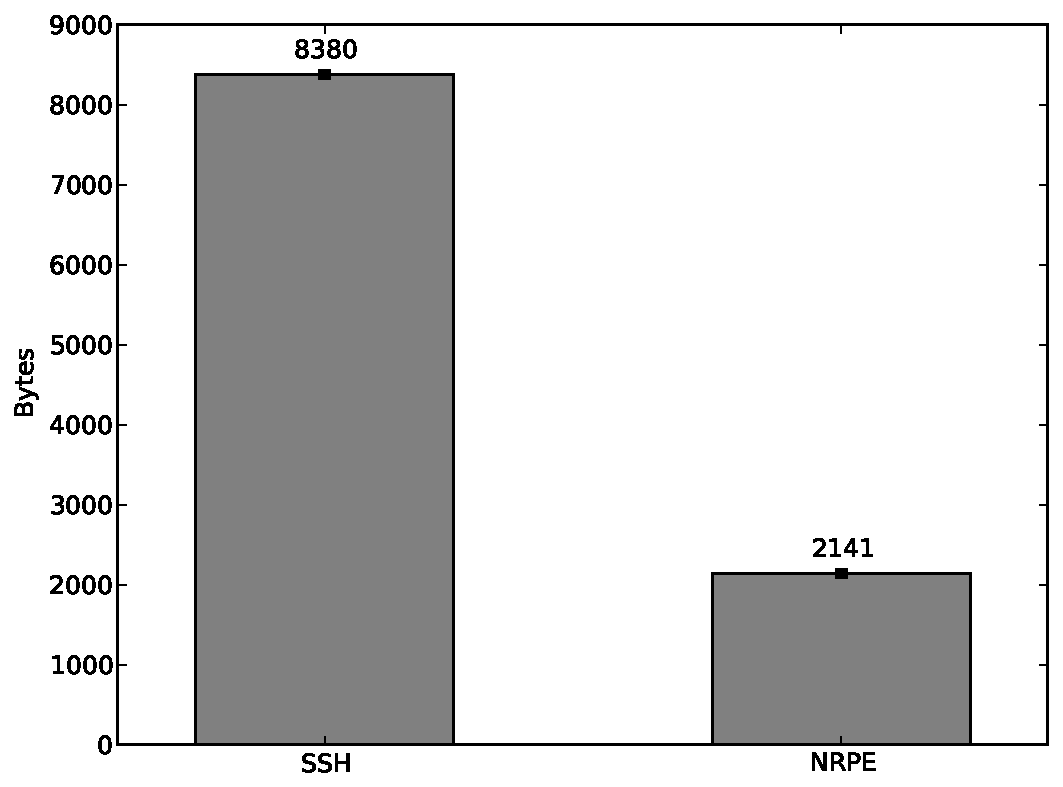
\includegraphics[scale=0.6]{img/nettverkstrafikk}
    \caption{Nettverkstrafikk}
    \label{network_traffic}
\end{figure}

\begin{figure}[H]
    \centering
    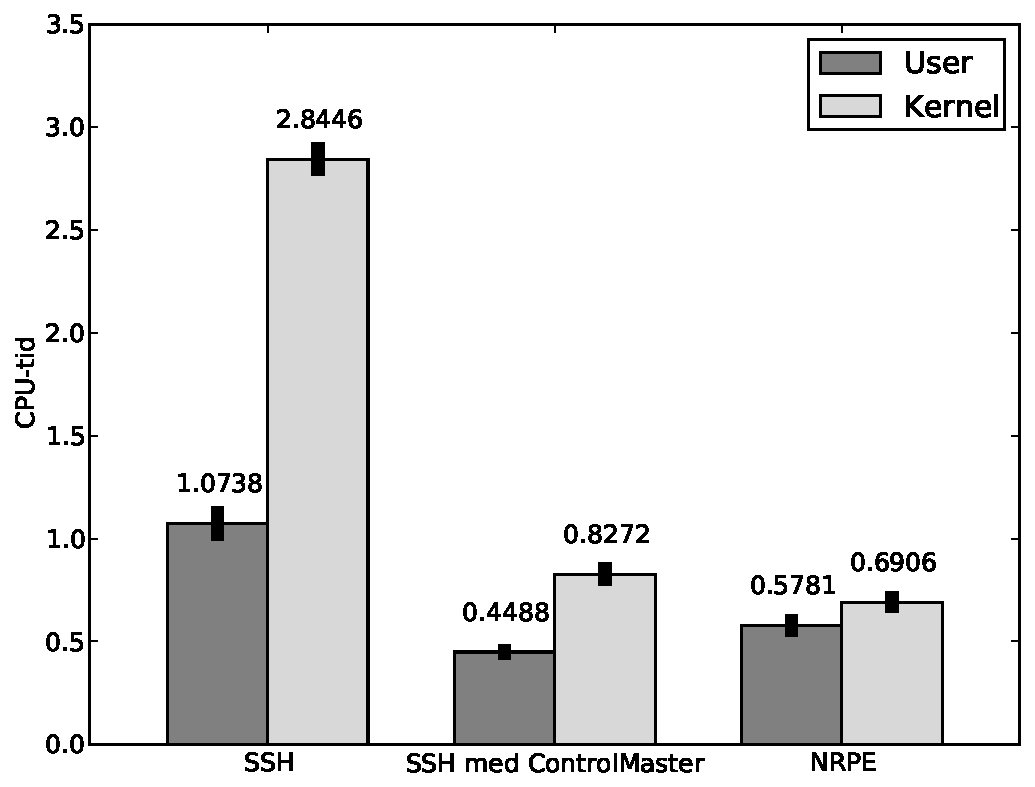
\includegraphics[scale=0.6]{img/cpubruk}
    \caption{CPU-bruk}
    \label{cpu_usage}
\end{figure}

\begin{table}
    \begin{center}
	\begin{threeparttable}
    \begin{tabular}{| l | l | l | l |} \hline
	\ & \textbf{CPU-tid i user(s)} & \textbf{CPU-tid i kernel(s)} & \textbf{Nettverkstrafikk (B)} \\ \hline
	SSH & 1.0738 (0.0792) & 2.8446 (0.0771) & 8380 (101.38) \\ \hline
	NRPE & 0.5781 (0.0347) & 0.6906 (0.0495) & 2141 (55.08) \\ \hline
	SSH med ControlMaster & 0.4488 (0.0509) & 0.8272 (0.0543) & 1700* \\ \hline
	\end{tabular}
	\begin{tablenotes}
	\small
	\item *For SSH med ControlMaster var det ikke mulig å separere ut hvor mye trafikk det var på én sjekk. Her er det brukt et gjennomsnitt ved å dele den totale mengden trafikk på antall sjekker.
	\end{tablenotes}
	\caption{Prosessorforbruk test med agenter}
	\label{agentcheck}
	\end{threeparttable}
	\end{center}
\end{table}
For en utrulling i den skalen som vil være aktuelt for IKT-avdelingen vil ikke denne nettverkstrafikken være noen stor faktor. Figur \ref{network_traffic} viser at gjennomsnittlig vil total båndbreddebruk for en sjekk var 8380 byte. Selv med 1000 enheter som overvåkes over SSH, der hver kjører 100 sjekker hvert 5. minutt, vil den totale båndbreddebruken, dersom alle sjekkene var jevnt fordelt over 5 minutters-intervallet:
\[\frac{8.38\:kB\times(1000\:(enheter)\times100\:(sjekker))\times8\:b/B}{5\:(min)\times60\:s}=22346.67\:Kb/s = 22.35\:Mb/s \] 
På et gigabit-nettverk, som i tillegg er full duplex, vil ikke dette være nevneverdig. Icinga vil forsøke å fordele sjekkene utover slik at lasten på Icinga-serveren og enhenetene som overvåkes blir minst mulig\cite{icingascheduling}, men i praksis blir ikke dette helt jevnt fordelt, tallet kan derfor bli noe høyere.

Resultatene av testen av CPU-tid i \ref{cpu_usage}, viser at SSH krever mer CPU-tid enn NRPE. Mye av dette er på grunn av overhead ved tilkobling og frakobling, som tallene for SSH med ControlMaster viser. 

Det ble valgt å benytte NRPE både for Linux- og Windows-servere. En fordel med dette er at samme protokoll for alle tilkoblinger fra Icinga-serveren til samme port (5666) på andre servere kan benyttes. Dette gjør at det kun trengs én brannmurregel for Icinga, som igjen holder antall angrepsvektorer nede. En annen fordel er at samme service- og command-objekter kan benyttes i Icinga for sjekker som skal utføres via NRPE, uavhengig av om hosten kjører Windows eller Linux.


%See page \pageref{status1.1} till \pageref{status2.1}.

\chapter{Implementasjon}
Dette kapittelet handler om hvordan gruppen har utført implementasjonen av overvåkningsløsningen for IKT-avdelingen, hvilke valg som er tatt underveis og hvordan de forskjellige enhetene overvåkes.
\clearpage
\section{Utstyr}
\subsubsection{Labmiljø}
Et labmiljø har vært brukt for å teste plugin-er og script før de ble implementert på produksjonsserveren. Ved å teste i et labmiljø først, kan en se hvordan sjekker oppfører seg, før de i stor skala implementeres i produksjon. Labmiljøet inneholder utstyr og tjenester som gjenspeiler det IKT-avdelingen benytter. På denne måten kan ulike scenarier og utstyr testes før dette settes i produksjon. I Tabell \ref{labmiljo} er det en oversikt over utstyret i labmiljøet.
\begin{changemargin}{-1cm}{-1cm}
\begin{table}[H]
\begin{center}
%\begin{tabular}{|p{2.0in}|c|c|c|} \hline
\begin{tabular}{ | l | l | l | p{4cm} |} \hline
	\textbf{Type} & \textbf{Beskrivelse} & \textbf{Dato installert} & \textbf{Tjenester} \\ \hline
	Server & Debian linux (HiG1) & 22.01.2013 & Icinga, Icinga-Web, Icinga-mobile, MySQL, Apache \\ \hline
	Server & Debian linux (HiG2) & 22.01.2013 &	MySQL, Apache \\ \hline
	Server & Windows 2008 R2 (HiG3) & 22.01.2013 & DNS, DHCP, AD, IIS, Fileserver, MSSQL \\ \hline
	Server & Windows 2008 R2 (HiG4) & 19.02.2013 & Exchange \\ \hline 
	Switch & Cisco 3550 (HiG-sw1) &	29.01.2013 & SNMP \\ \hline
	Switch & Dell Powerconnect 5324 (HiG-sw2) & 29.01.2013 & SNMP \\ \hline
	Router & Cisco 2600 (HiG-ro) & 05.02.2013 & SNMP \\ \hline 
	Firewall & Cisco 515E (HiG-fw) & 05.02.2013 & SNMP \\ \hline
\end{tabular}
\caption{Labmiljø}
\label{labmiljo}
\end{center}
\end{table}
\end{changemargin}
Serverne er virtuelle maskiner i et eget VLAN, som er tilgjengelig på fysiske porter, slik at nettverksutstyret kan plasseres i samme nettverk. VLAN-et har også tilgang ut mot Internett og har vært tilgjengelig for gruppen over VPN. Tjenester som testes på HiG1, HiG2, HiG3 og HiG4 blir alle overvåket via NRPE. For nettverksutstyret blir SNMP benyttet.

I Figur \ref{laboppsett} vises det logiske oppsettet av labmiljøet. I Tabell \ref{labmiljo} vises hvilke tjenester som kjøres. HiG-fw, HiG-sw1 og HiG-sw2 er koblet i serie for å teste avhengigheter og følgefeil.

\begin{figure}[H]
    \centering
    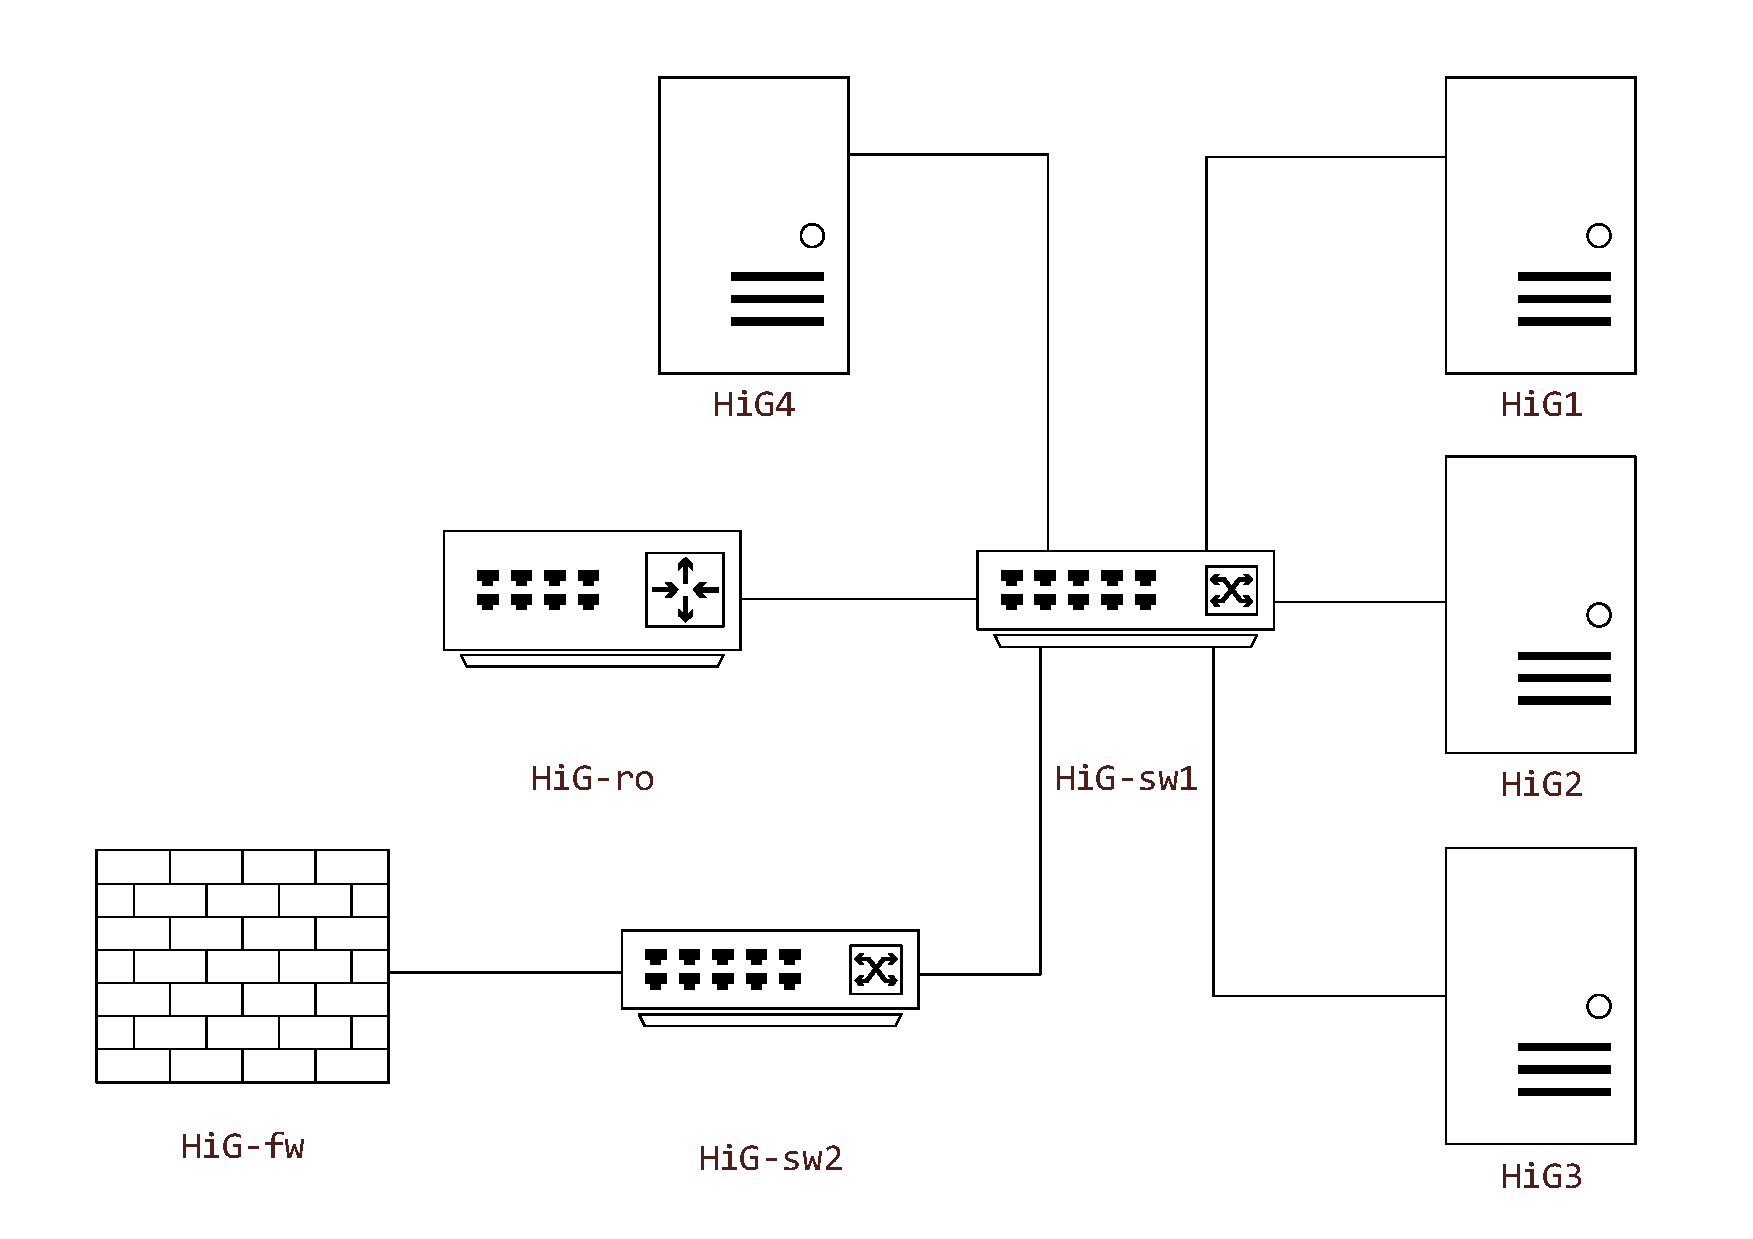
\includegraphics[scale=0.4]{img/labmiljo}
	\label{laboppsett}
    \caption{Labmiljø}
\end{figure}

\subsubsection{Produksjonsserveren}
Spesifikasjonene på bladeserveren:
\begin{itemize*}
\item 4 CPU-er med 4 kjerner à 2.4 GHz
\item 32 GB RAM
\end{itemize*}
Programvare:
\begin{itemize*}
\item Debian 6
\item Apache2
\item MySQL
\item Icinga 1.8.4
\item SNMPtrapd
\item SNMPtt
\item Graphite
\item Metricinga 
\item sendmail
\end{itemize*}

\subsubsection{Enhet for overvåkning av servermiljø}
For å overvåke temperatur og luftfuktighet på serverrommet ble det i samråd med IKT-avdelingen kjøpt inn en APC NetBotz 200, som støtter opptil 12 eksterne sensorer\cite{netbotz}. Denne oppfyller kravene gitt i oppgavebeskrivelsen. 

\section{Produksjonsserver}
``Quis custodiet ipsos custodes?'' er et latinsk uttrykk som kan oversettes med ``hvem passer på de som passer på?''. I en overvåkningsløsning er det viktig å stille spørsmålet; hva skjer hvis overvåkningsserveren går ned? Et forslag ved starten av prosjektet var å legge overvåkningsserveren på et Xen- eller VMware-cluster. Men dette ble etter noe omtanke stemplet som en dårlig idé. Dersom clusteret gikk ned, ville også overvåkningsserveren gå ned. Det ble derfor bestemt at Icinga-serveren skulle være en egen fysisk server, med databasen installert lokalt.

For å sikre tilgjengeligheten til Icinga ytterligere, er det også mulig å sette opp et redundant oppsett der alle Icinga-installasjoner kan dele resultater av sjekker mellom seg. Ekstra viktig vil et slikt oppsett være dersom en knytter overvåkningssystemet mot SLA-er. Dersom en mister data om oppetid og tilgjenglighet på en tjeneste, vil en ikke lenger kunne vise hva den har vært.

En annen utfordring var å vite hvor kraftig hardware serveren trengte. Her ble referanselisten til Icinga lagt til grunn, hvor mange organisasjoner har lagt inn informasjon om sine oppsett\cite{icingainaction}. Etter avtale med oppdragsgiver ble det bestemt å sette opp en bladeserver, som kan oppgraderes dersom det skulle bli nødvendig. 

Debian 6 ble valgt som operativsystem på Icinga-serveren etter ønske fra oppdragsgiver. 
\subsection{Installasjon}
Ved starten av iterasjonen ``kjerneprogramvare'' var den nyeste versjonen av Icinga 1.8.4. I pakkebrønnen for debian-stable fantes bare versjon 1.0.2 av Icinga, i backports lå 1.7.1. Icinga opprettholder en egen pakkebrønn - ``The Debian Monitoring Project'' (debmon\cite{debmon}). Fra denne kunne versjon 1.8.4 installeres. I samråd med teknisk kontakt ved IKT-avdelingen ble det bestemt å bruke versjon 1.8.4 fra debmon.

\subsubsection{Icinga Webgrensesnitt}
Webgrensesnittene Icinga Classic og Icinga Web ble installert med pakkene ``icinga-classic'' og ``icinga-web 1.8.1'', via pakkebrønnen debmon. 

Tidlig ble det avgjort at Icinga Web primært skulle brukes som webgrensesnitt mot Icinga. Denne avgjørelsen ble tatt fordi Icinga Web kommer med et REST-API, har støtte for LDAP-integrasjon og aksesstyring på mange objekter.

Etter testing ble det oppdaget at Icinga Web opplevdes som mye tregere enn Icinga Classic og inneholder en feil som ble rapportert tilbake til Icinga Development Team. Feilen som ble rapportert inn omfatter søk på hostgroup-objekter eller servicegroup-objekter (bugreport\cite{icingawebbug}). Det ble derfor lagt opp til at både Icinga Classic og Icinga Web kan benyttes på lik linje.
\subsection{Konfigurasjonsfiler}
Ved standard installasjon av Icinga er konfigurasjonen delt opp i objekttyper med flere objekter i hver fil:
\begin{itemize*}
\item contacts\_icinga.cfg  
\item generic-host\_icinga.cfg     
\item hostgroups\_icinga.cfg  
\item localhost\_icinga.cfg  
\item timeperiods\_icinga.cfg
\item extinfo\_icinga.cfg   
\item generic-service\_icinga.cfg   
\item services\_icinga.cfg
\item commands.cfg
\end{itemize*}
Dette var uoversiktlig og en mer oppdelt konfigurasjon var ønskelig, som også er anbefalt ved større installasjoner\cite{nagiosenterprise,sysadmin}. Derfor ble det bestemt å sette opp følgende hovedinndeling (med undermapper videre der det var hensiktsmessig):

\makeatletter
\newcount\dirtree@lvl
\newcount\dirtree@plvl
\newcount\dirtree@clvl
\def\dirtree@growth{%
  \ifnum\tikznumberofcurrentchild=1\relax
  \global\advance\dirtree@plvl by 1
  \expandafter\xdef\csname dirtree@p@\the\dirtree@plvl\endcsname{\the\dirtree@lvl}
  \fi
  \global\advance\dirtree@lvl by 1\relax
  \dirtree@clvl=\dirtree@lvl
  \advance\dirtree@clvl by -\csname dirtree@p@\the\dirtree@plvl\endcsname
  \pgf@xa=0.5cm\relax
  \pgf@ya=-0.5cm\relax
  \pgf@ya=\dirtree@clvl\pgf@ya
  \pgftransformshift{\pgfqpoint{\the\pgf@xa}{\the\pgf@ya}}%
  \ifnum\tikznumberofcurrentchild=\tikznumberofchildren
  \global\advance\dirtree@plvl by -1
  \fi
}

\tikzset{
  dirtree/.style={
    growth function=\dirtree@growth,
    every node/.style={anchor=north},
    every child node/.style={anchor=west},
    edge from parent path={(\tikzparentnode\tikzparentanchor) |- (\tikzchildnode\tikzchildanchor)}
  }
}
\makeatother
\begin{tikzpicture}[dirtree]
\node {Objects} 
    child { node {commands}
            child { node {firewalls} }
            child { node {servers} }
            child { node {switches} }
    }
    child { node {contactgroups} }
    child { node {escalations} }
    child { node {generics} }
    child { node {hostdependencies} }
    child { node {hostgroups} }
    child { node {hosts} }
    child { node {modules} }
    child { node {servicedependencies} }
    child { node {services} };
\end{tikzpicture}

Det ble testet ut et par verktøy for å administrere konfigurasjonsfilene, NConf\cite{nconf} og NagiosQL\cite{nagiosql} i et webgrensesnitt. Disse ble valgt bort til fordel for manuell konfigurering, da oppdeling av konfigurasjonen ikke var støttet, og de kunne ikke kombineres med manuell konfigurering. I samråd med oppdragsgiver ble det avgjort at manuell konfigurasjon oppfyller kravet om at det skal være enkelt å legge til nye enheter for overvåking.

\subsection{Bruk av hostgroup}
Som nevnt i \ref{sec:objekter} knyttes et service-objekt til et host-objekt og et command-objekt, for at det skal kjøres en sjekk. For å slippe å skrive et service-objekt for hvert nytt host-objekt, benyttes gruppering av host-objekter i en hostgroup. Under vises et eksempel på hvordan dette er satt opp for MySQL-servere. 

Først defineres en hostgroup for alle SQL serverne. Dette gjøres for å gruppere alle SQL serverne uavhengig av hvilken databasetype som brukes. 
\begin{lstlisting}[style=example]
define hostgroup {
    hostgroup_name		sql_servers
    alias         		SQL Servers
    hostgroup_members	mysql_servers, mssql_servers, oracle_servers
}
\end{lstlisting}
Deretter defineres en hostgroup for alle MySQL-servere.
\begin{lstlisting}[style=example]
define hostgroup {
    hostgroup_name 		mysql_servers
    alias         		MySQL Servers
}
\end{lstlisting}
For å legge til en host i denne gruppen kan host-objektet være definert på følgende måte.
\begin{lstlisting}[style=example]
define host {
    use				generic_linux_host
    address			10.60.0.21
    host_name		HiG2
    alias    		HiG2
    hostgroups		debian_servers, mysql_servers
}
\end{lstlisting}
Service-objektet defineres slik og refererer til hostgroup-en og kommandoen ``check\_mysql\_health''. Alle host-objekter i ``mysql\_servers'' vil da få denne sjekken.
\begin{lstlisting}[style=example]
define service {
    service_description	MySQL Connection Time
    use		 			generic_service
    name 				mysql_connection_time
    hostgroup_name 		mysql_servers
    check_command 		check_mysql_health!connection-time!0.1!0.4
}
\end{lstlisting}

Figur \ref{sql} viser en visuell fremstilling av hvordan dette henger sammen for alle SQL-servere:
\begin{changemargin}{-1cm}{-1cm}
\begin{figure}[H]
    \centering
    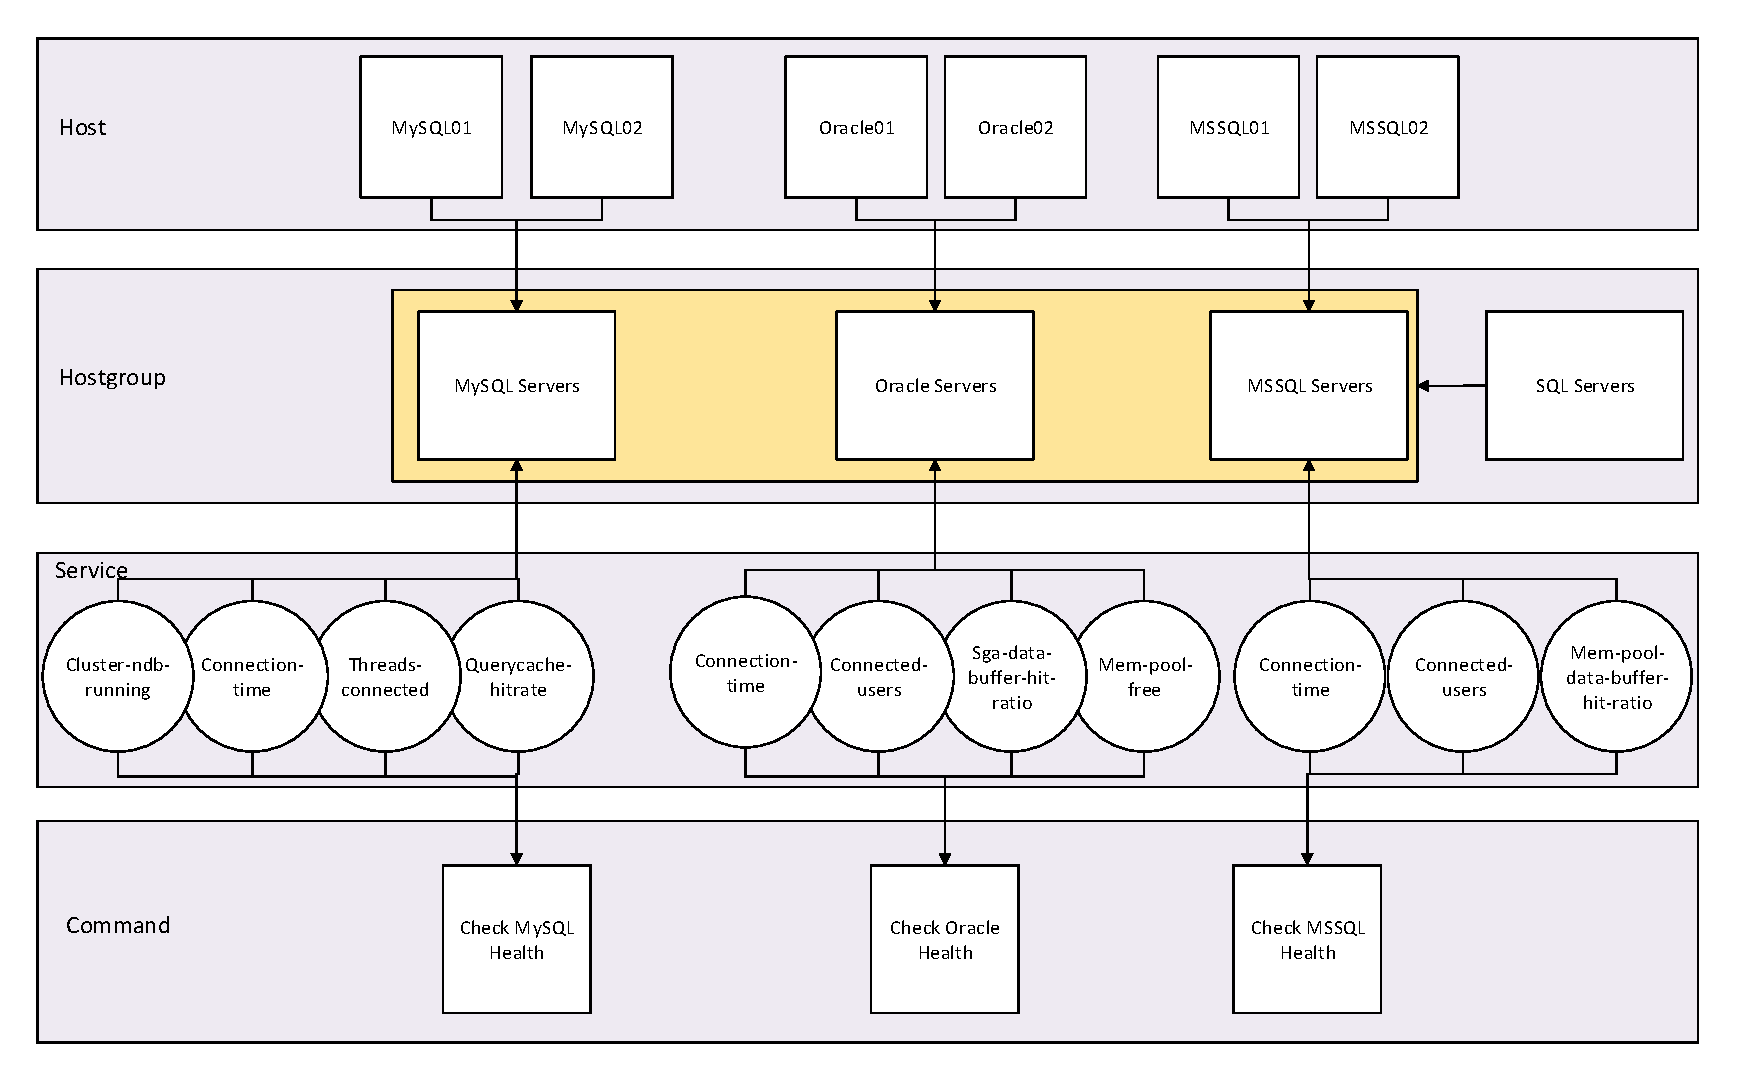
\includegraphics[scale=0.55]{img/sql}
    \caption{Visualisering av konfigurasjon av SQL-servere}
    \label{sql}
\end{figure}
\end{changemargin}
\clearpage

\section{Generering av grafer}
I utgangspunktet ble det bestemt at ytelsesdata skulle holdes utenfor oppgaven. Det ble likevel satt opp en løsning for å visualisere ytelsesdata fra sjekkene med programmet Graphite\cite{graphite}. Dette ble gjort fordi det var ønskelig å kunne etablere en baseline for tjenestene slik at bedre grenseverdier kunne settes.

For å sette opp eksportering av ytelsesdataen benyttes et vanlig command-objekt i Icinga:
\begin{lstlisting}[style=example]
define command {
    command_name	rotate_perf_service
    command_line	/bin/mv /usr/local/icinga/var/perfdata/service-perfdata /usr/local/icinga/var/perfdata/logs/service-perfdata.$TIMET$
}
\end{lstlisting}

Icinga.cfg må konfigureres til å benytte dette:
\begin{lstlisting}[style=example]
process_performance_data=1
service_perfdata_file=/usr/local/icinga/var/perfdata/service-perfdata
service_perfdata_file_processing_command=rotate_perf_service
service_perfdata_file_template=[SERVICEPERFDATA]\tDATATYPE::SERVICEPERFDATA\tTIMET::$TIMET$\tHOSTNAME::$HOSTNAME$\tSERVICEDESC::$SERVICEDESC$\tSERVICEPERFDATA::$SERVICEPERFDATA$service_perfdata_file_processing_interval=200
\end{lstlisting}

For å transformere ytelsesdataene til riktig format for Graphite benyttes ``Metricinga''\cite{metricinga}. Dette scriptet sjekker ``spool''-mappen som command-objektet flytter filene med ytelsesdata til. Metricinga sjekker mappen én gang i minuttet etter filer som enda ikke er prosessert, og sender data inn til Graphite (via carbon). Gjennom Graphite vil det dermed genereres grafer basert på ytelsesdata fra alle service-sjekker som gir dette.

Det ble også testet å modifisere scriptet til å lagre outputen til service-sjekkene direkte i en MySQL-database, som vist i Vedlegg \ref{diff.pl}. Dette ble gjort for å oppfylle kravet fra oppgavebeskrivelsen om at alle henvendelser skal lagres i database. I samråd med oppdragsgiver ble det avgjort å gå bort i fra dette fordi det resulterte i et høyt antall nye rader over kort tid. Som et alternativ til dette kan en ta inn all data til Graphite, men aggregere det etter en viss tid. For eksempel lagre dagsgjennomsnittet for data som er eldre enn seks måneder. Dataene kan da eksporteres fra Graphite til videre bruk.

Metricinga kommer ikke med init-script for Debian. For at prosessen skal kunne startes automatisk med serveren ble dette skrevet av gruppen (Vedlegg \ref{metricinga_init.d}).
\section{Overvåkning av Windows-servere}
For overvåkning av Windows-servere brukes programmet NSClient++\cite{nsclientmain}. Programmet brukes for å kommunisere med ulike agenter over ulike protokoller på en ekstern server. I dette prosjektet brukes NSClient++ til å hente ut informasjon via NRPE-agenten og å kjøre WMI-spørringer mot en Windows-server. 

Under installasjon av NSClient++ blir en standard konfigurasjonsfil generert. Her derfineres hvilke IP-adresser som kan koble seg til, og hvilke sjekker som er tilgjengelige.

NSClient++ er valgt fordi klienten oppdateres hyppig \cite{nsclient}, og det er den agenten som blir referert i Icinga/Nagios dokumentasjon \cite{icingawin}. Med NSClient++ kommer også forhåndskonfigurerte plugin-er, for eksempel for å sjekke CPU, minne og harddiskplass.

\section{Overvåkning av Linux-servere}\label{sec:overvaklinux}
Overvåkning av Linux-servere skjer utelukkende ved bruk av NRPE. For Debian-servere kan en NRPE-daemon installers fra pakkebrønnen ``stable'' med kommandoen:
\begin{lstlisting}[style=example]
apt-get install nagios-nrpe-server nagios-plugins-basic
\end{lstlisting}

For Red Hat og CentOS må det installeres en tredjeparts pakkebrønn som ``EPEL'' eller ``DAG'' før nrpe-server kan installeres med yum.

Ved bruk av DAG må ``rpm''-pakken ``rpmforge'' installeres for å kunne bruke pakkebrønnen, slik:
\begin{lstlisting}[style=example]
rpm -Uvh http://apt.sw.be/redhat/el6/en/x86_64/rpmforge/RPMS/rpmforge-release-0.5.2-2.el6.rf.x86_64.rpm
\end{lstlisting}

For EPEL må pakken ``epel'' installeres:
\begin{lstlisting}[style=example]
sudo rpm -Uvh http://dl.fedoraproject.org/pub/epel/6/x86_64/epel-release-6-8.noarch.rpm
\end{lstlisting}

En kan verifisere at pakkebrønnene ble lagt til ved å kjøre en listing av direktivet /etc/yum.repos.d/:
\begin{lstlisting}[style=example]
$ ls -1 /etc/yum.repos.d/epel*
/etc/yum.repos.d/epel.repo
/etc/yum.repos.d/epel-testing.repo
\end{lstlisting}

Installasjon av NRPE via yum etter at pakkebrønnene er lagt til:
\begin{lstlisting}[style=example]
sudo yum install nagios-nrpe-2.12-1.el6.rf.x86_64.rpm nagios-plugins
\end{lstlisting}

Eksemplene er for CentOS og RHEL 6.x 64-bit.

Konfigurasjonen på Linux-servere skjer på samme måte som på Windows-servere. Det følger ikke med noen plugin-er når en installerer nagios-nrpe-server, derfor installeres også den offisielle plugin-pakken for Nagios. I debian heter denne pakken ``nagios-plugins-basic'', og for Red Hat/CentOS ``nagios-plugins''.

\section{Utrulling av agenter}
NSClient++ kan lastes ned som en MSI-pakke, som kan distribueres til servere med en GPO. Konfigurasjonsfilen må enten legges inn i MSI-pakken eller pushes over GPO for seg selv. Det ble laget en veiledning på hvordan denne klienten skal installeres, og hvilke opsjoner som er relevante. Denne finnes i Vedlegg \ref{agentguide}.

For Linux-servere installeres pakkene via pakkebehandleren, som nevnt i \ref{sec:overvaklinux}. For utrulling kan et script som kobler seg til og kjører kommandoen for installering skrives. Konfigurasjonsfilen kan pushes over SCP.

Distribuering er ikke benyttet fordi IKT-avdelingen ønsker å gjøre installasjonen manuelt for å ha mest mulig kontroll, sikre seg mot uforutsette problemer og gjøre utrulling i faser.
 
For annen infrastruktur brukes for det meste SNMP for å hente ut informasjon. Dette konfigureres på hver enkelt enhet, og krever ikke noe ekstra programvare installert. I noen tilfeller brukes egne API-er for å hente ut informasjon, som for eksempel for VMware. Her må Icinga serveren ha tilgang til å bruke API-et, som konfigureres på Virtual Center-serveren.

\section{Lokale ressurser}\label{sec:lokaleressurser}
For både Linux- og Windows-servere er det satt opp noen grunnsjekker som skal kjøres på alle servere. Dette er CPU-last, harddiskplass og minnebruk. Hver av sjekkene er definert i et service-objekt der hostgroup-ene er satt til ``windows\_servers'' og ``linux\_servers''. 

For alle disse sjekkene er det mulig å angi grenseverdier både som prosentandel og absolutte tall. Det kan også sjekkes mot både andel ledig og andel brukt. 
\subsection{CPU}
Overvåkning av CPU vil kunne hjelpe til med å oppdage ressursproblemer. Dette kan komme av flere CPU-krevende applikasjoner på samme server, eller at en applikasjon bruker all CPU-kraft.  

På Windows-servere benyttes ``CheckCPU'' fra NSClient++ for å sjekke CPU-last over NRPE. Her legges det ved tre opsjoner i sjekken som spesifiserer tidsintervallet for datagrunnlaget, grenseverdi for når det skal gis en WARNING og grenseverdi for CRITICAL.

Kommandoen for plugin-en slik den er definert i command-objektet. Dette henter et gjennomsnittsbruk av CPU over 5 minutter: 
\begin{lstlisting}[style=example]
./check_nrpe -u -H 10.60.0.22 -p 5666 -c CheckCPU -a time=5m warn=80 crit=90
\end{lstlisting}
Svar:
\begin{lstlisting}[style=example]
OK CPU Load ok.|'5m'=0%;80;90
\end{lstlisting}

I Figur \ref{cpuok} vises svaret fra CPU-sjekken i Icinga. 
\begin{figure}[H]
    \centering
    
\includegraphics[scale=0.8]{img/HiG3_cpu_ok}
    \caption{Visning av en CPU-sjekk som gir OK i Icinga}
    \label{cpuok}
\end{figure}

I Figur \ref{cpucritical} ser vi at sjekken gir en CRITICAL-tilstand på service-objektet, på grunn av et gjennomsnittsbruk av CPU på 96 \%. 
\begin{figure}[H]
    \centering
    
\includegraphics[scale=0.8]{img/HiG3_cpu_critical}
    \caption{Visning av en CPU-sjekk som gir CRITICAL i Icinga}
    \label{cpucritical}
\end{figure}

I Figur \ref{cpustrain} ser vi at alle de fire CPU-kjernene jobber opp mot maksimalt. Et Batch-script ble kjørt lokalt på serveren som ble overvåket for å generere CPU-bruk.
\begin{lstlisting}[style=example]
## winloop.bat
##
# Runs loop.bat 10 times.
#
@echo off
for /l %%x in (1, 1, 10) do (
    start loop.bat
)

# loop.bat
@echo off
:loop
GOTO loop
\end{lstlisting}

\begin{figure}[H]
    \centering
    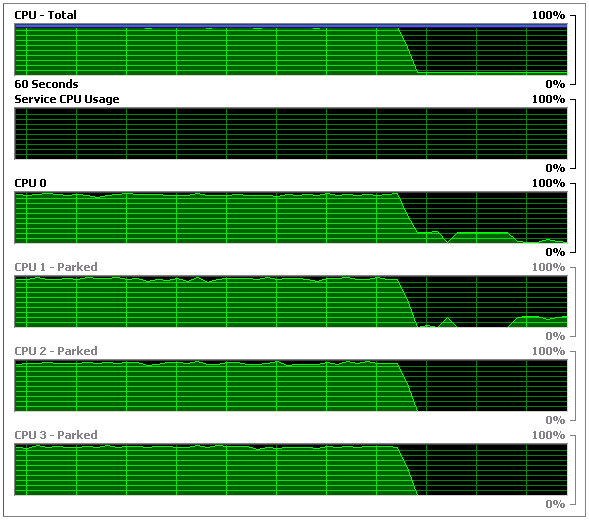
\includegraphics[scale=0.6]{img/HiG3_cpu_graph}
    \caption{CPU-bruk for HiG3}
    \label{cpustrain}
\end{figure}

På Linux-servere baserer sjekk av CPU-bruk seg på ``load-average'' \cite{loadavg, wiki:loadavg}. Dette er i hovedsak et gjennomsnitt for hvor mange prosesser som bruker eller venter på CPU-en, men disk- eller nettverks-I/O kan også spille inn. For servere med flere kjerner vil dette fortone seg annerledes da en kan utføre flere prosesser parallelt. Load-tallene må deles på antallet CPU-kjerner for at det skal kunne brukes samme grenseverdier uavhengig av hvor mange kjerner serveren har. Dette gjøres med opsjonen ``r''.

Tallene som hentes ut er gjennomsnittet for de siste 1, 5 og 15 minuttene. Det er mer interessant hvis load-en er høy over lengre tid, derfor er grenseverdiene lavere for 5 og 15 minutters intervallene. Eksempel på load-tall: {\bf load average}: 0.65 0.42 0.36.

check\_load fra nagios-plugins:
I service-objektet:
\begin{lstlisting}[style=example]
check_command check_nrpe!check_dist_load!0.9,0.7,0.5 1.2,1.0,0.9
\end{lstlisting}
Kommando brukt i command-objektet check\_dist\_load:
\begin{lstlisting}[style=example]
/check_load -r -w $ARG1$ -c $ARG2$
\end{lstlisting}

\subsection{Minne}
Datamaskiner som bruker opp tilgjengelig minne må skrive til disk for å få plass til mellomlagrede data. Data som må hentes fra disk vil ha en betydelig høyere aksesstid enn når RAM brukes til mellomlagring \cite{wiki:mem}. 
Kontinuerlig høyt minneforbruk kan være en indikasjon på flere minnekrevende applikasjoner på samme server, at en applikasjon har minnelekkasje, eller at mengden minne ikke strekker til.

For Windows-servere brukes CheckMem fra NSClient++
\begin{lstlisting}[style=example]
./check_nrpe -u -H 10.60.0.22 -p 5666 -c CheckMem -a MaxWarnUsed=80% MaxCritUsed=90% type=physical
\end{lstlisting}
Svar:
\begin{lstlisting}[style=example]
OK memory within bounds.|'physical memory %'=16%;80;90 'physical memory'=1G;4;5;0;6
\end{lstlisting}

For Linux benyttes plugin-en check\_mem \cite{checklinuxmem}, da det ikke følger med noen plugin for å sjekke minneforbruk i nagios-plugins.
\begin{lstlisting}[style=example]
   check_command    check_nrpe!check_mem!80 90 ; Check that percent used is within tresholds. Used is calculated from total - free - cached - buffers 
                    command[check_mem]=/usr/lib/nagios/plugins/libexec/check_mem.pl -w $ARG1$ -c $ARG2$
\end{lstlisting}
\subsection{Disk}
En full harddisk kan skape problemer for applikasjoner som lagrer data og logger fra systemet kan stoppe. Ved høyt minneforbruk og bruk av virtuelt minne i kombinasjon med en full disk, vil ikke harddisken kunne utnyttes som swap, og applikasjoner kan stoppe å fungere.

For Windows-servere benyttes ``CheckDisk'' fra NSClient++. For å sjekke flere disker brukes opsjonen ``CHECKALL'', som gir en oversikt over alle diskene på serveren.

\begin{lstlisting}[style=example]
./check_nrpe -u -H 10.60.0.22 -p 5666 -c CheckDriveSize -a Drive="C" MaxWarnUsed=90% MaxCritUsed=95%
./check_nrpe -u -H 10.60.0.22 -p 5666 -c CheckDriveSize -a MaxWarnUsed=94% MaxCritUsed=96% CheckAll
\end{lstlisting}

For Linux-servere benyttes sjekken ``check\_disk'' fra nagios-plugins. Her spesifiseres baner som er montert i filsystemet.

check\_disk kjøres slik:
\begin{lstlisting}[style=example]
./check_disk -w 8% -c 4% --mountpoint --all
\end{lstlisting}
Svar: 
\begin{lstlisting}[style=example]
DISK OK| /=1232MB;15430;17359;0;19288 /lib/init/rw=0MB;402;452;0;503 /dev=0MB;394;443;0;493 /dev/shm=0MB;402;452;0;503
\end{lstlisting}

\section{Tjenester}
IKT-avdelingen ønsket å overvåke tjenester og prosesser på serverne. Prossesser er instanser av programmer som kjører. Tjenester er prosesser som kjører i bakgrunnen. 

Overvåkning av tjenester vil innebære å se på om en eller flere prosesser kjører til en hver tid. NSClient++ har muligheten til å se om en bestemt tjeneste kjører eller har stoppet gjennom ``CheckServiceState''. Her spesifiserers navnet på tjenesten, og sjekken svarer på om denne tjensten kjører.
\begin{lstlisting}[style=example]
define service {
    service_description     DHCP Service
    hostgroup_name          dhcp_servers
    check_command           check_nrpe!CheckServiceState!DHCPServer=started ShowAll
    use                     generic_service
}
\end{lstlisting}
For Linux brukes plugin-en ``check\_procs'' fra nagios-plugins. For denne plugin-en spesifiseres også hvor mange instanser av prosessen som skal forekomme. 
\begin{lstlisting}[style=example]
define service {
    use            	        generic_service
    hostgroup_name       	linux_servers
    service_description     	NRPE Check my process
    check_command        	check_nrpe!check_process!sshd 1:40
}
\end{lstlisting}

Å se at en tjeneste kjører via Windows kan gi falsk informasjon. Et eksempel på dette er  at tjenesten ``Microsofts terminal services'' står som kjørende i Windows, men brukere får ikke koblet til. Dette kommer av at tjenesten har hengt seg, uten at den står som ``stoppet''. Dette merkes ikke før brukere ringer inn og beskriver problemet\cite{serviceproblem}. Som nevnt i \ref{sec:omovervakning} vil en bedre sjekk være å teste selve tjenesten. Dette gjøres for alle tjenestene beskrevet i de neste delkapitlene.

\subsection{LDAP, DNS og DHCP}
Tjenester som LDAP-autentisering, DNS-oppslag og DHCP-leasing er en viktig del av tjenestene IKT-avdelingen leverer.

LDAP-tjenesten\cite{ldap} gjør at brukere får logget på trådløse nettverk og autentisert seg for andre tjenester IKT-avdelingen leverer.

DNS-oppslag gjøres hver gang en enhet skal oversette en IP-adresse til et hostname eller omvendt. Uten DNS vil ikke enheten kunne kontakte andre enheter ved å benytte hostname, som brukes i eksempelvis web-adresser\cite{dns}. 

Når en ny enhet kobles til nettverket vil denne få tildelt en IP-adresse av DHCP-serveren. Samtidig får den informasjon om gateway og DNS-servere. Uten dette vil ikke enheten få kommunisert med andre enheter på det lokale nettverket og Internett\cite{dhcp}.

Sjekkene for alle de tre tjenestene vil bli gjort direkte fra Icinga-serveren. Denne står i et eget nettverk. Derfor vil det kunne oppstå situasjoner der Icinga rapporterer at tjenestene fungerer, men det fungerer ikke for brukere tilkoblet andre nettverk. En løsning på dette kan være å kjøre sjekkene via en server i hvert nettverk hvor brukere er tilkoblet.

\subsubsection*{LDAP}
For å overvåke LDAP-tjenestene benyttes plugin-en ``check\_ldap'' som følger med i nagios-plugins. Plugin-en kobler til LDAP-tjenesten og prøver å autentisere en spesifisert bruker. Her vil sjekken returnere OK, om den fikk koblet til og autentisert. 

Ytelsesdata har blitt samlet inn over 30 dager, for å sette grenseverdier for når Icinga skal gi varsel om treg innlogging. I Figur \ref{ldapauth-inv} vises det at tjenesten sjekket på fire LDAP-servere, over en måneds periode bruker rundt 0.0044 sekunder på å autentisere. Ut ifra dataen som er samlet inn settes grenseverdien for WARNING til 0.01 sekund, og CRITICAL til 0.02 sekunder.

\begin{figure}[H]
    \centering
    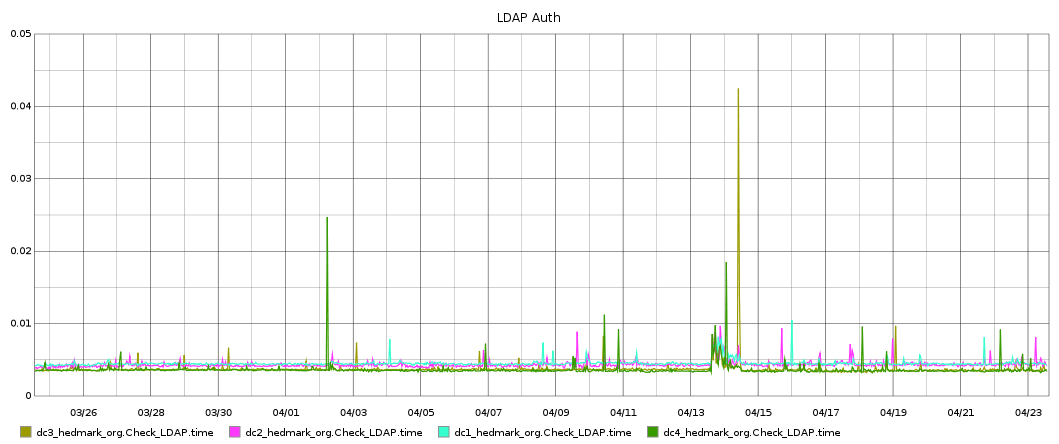
\includegraphics[width=1.0\textwidth]{img/ldap-auth-inv}
    \caption{Ytelsesdata i sekunder ved LDAP-autentisering}
    \label{ldapauth-inv}
\end{figure}
\begin{lstlisting} [style=example]
    check_command 	check_ldap_status!0.05!0.1!10
    command_line    	$USER1$/check_ldap -H $HOSTADDRESS$ -b $USER6$ -P $USER4$ -w $ARG1 -c $ARG2 -t $ARG
\end{lstlisting}

\subsubsection*{DNS}
DNS overvåkes med plugin-en ``check\_dns''. Denne, på samme måte som check\_ldap kobler seg til selve tjenesten. Dette fungerer ved å gjøre et DNS-oppslag på en spesifikk IP-adresse, og verifisere dette mot et satt hostname. Dersom dette stemmer vil plugin-en returnere OK, sammen med ytelses-data på hvor lang tid oppslaget tok.

Figur \ref{dns-inv} viser data samlet inn fra to DNS servere over 30 dager. Disse dataene viser forventet tid for et oppslag, og ut ifra dette ble grenseverdien for WARNING satt til 0.01 sek og CRITICAL til 0.02 sek.

\begin{figure}[H]
    \centering
    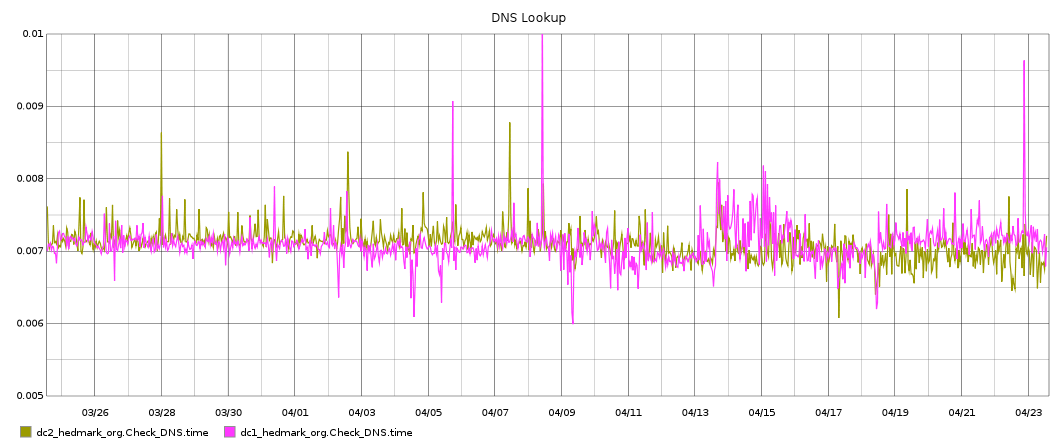
\includegraphics[width=1.0\textwidth]{img/dns-inv}
    \caption{Ytelsesdata i sekunder ved DNS-oppslag}
    \label{dns-inv}
\end{figure}

\begin{lstlisting} [style=example]
    check_command	check_dns_status!$HOSTNAME$!0.1!0.2!10
    command_line	$USER1$/check_dns -s $HOSTADDRESS$ -H $ARG1$ -w $ARG2$ -c $ARG3$ -t $ARG4$ -A
\end{lstlisting}

\subsubsection*{DHCP}
Overvåkning av en DHCP-tjeneste ble testet i labmiljøet med plugin-en ``check\_dhcp''. Denne sender en DHCPDISCOVER-pakke til DHCP-serveren. Hvis DHCP-tjenesten fungerer får plugin-en en DHCPOFFER-pakke som respons. Dersom denne inneholder en korrekt lease, returnerer plugin-en OK til Icinga sammen med tiden det tok.

\begin{lstlisting} [style=example]
;   check_command	check_nrpe!CheckServiceState!DHCPServer=started ShowAll
    command_line	$USER1$/check_dhcp -s 10.60.0.22
\end{lstlisting}

\subsection{Webservere}\label{sec:webservere}
IKT-avdelingen drifter mange webservere som benyttes av, eller gir informasjon til brukere. Plugin-en ``check\_http'' \cite{checkhttp} fra nagios-plugins benyttes for å sjekke at tilkoblingen til webserveren svarer på henvendelsen. Deler av forventet innhold sjekkes for å se at websiden ikke har blitt endret av uvedkommende.

Kommandoen for å gjøre dette er for siden http://portal.hedmark.org:
\begin{lstlisting}[style=example]
./check_http -H portal.hedmark.org -s "Velkommen til Hedmark fylkeskommunes portal" -S 
\end{lstlisting}

For websider som skal svare via HTTPS, sjekkes også utløpsdato for SSL-sertifikatet. I eksempelet under vil plugin-en gi en WARNING om sertifikatet utløper innen 50 dager:
\begin{lstlisting}[style=example]
./check_http -H portal.hedmark.org -C 50
\end{lstlisting}

\subsection{Terminalservere}\label{sec:terminalservere}
Mange interne applikasjoner kjøres via terminalservere. Det er viktig at terminalserverne er stabile fordi hver enkelt brukes som en lokal maskin av mange brukere. Ofte kan terminalservere belastes mer i perioder, derfor overvåkes hvor mange aktive brukere som er tilkoblet. Da kan en se hvilke som er mest belastet og når det er behov for å sette inn flere servere.

Antallet aktive og inaktive brukere kan hentes ut fra Windows Performance Counters. Disse overvåkes over NRPE med check\_counter i NSClient++. I Figur \ref{ts-skole-usage} er bruken for en måned uke samlet inn. Ut ifra bruken over en måned er WARNING og CRITICAL satt til 25 og 35 for å varsle unormal bruk.

Kommando som er brukt for å sjekke antallet aktive brukere på en terminalserver er:
\begin{lstlisting}[style=example]
./command_line check_nrpe -u -H $HOSTADDRESS$ -p 5666 -c CheckCounter -a "Counter:Active=\\Terminal Services\\Active Sessions" ShowAll MaxWarn=25 MaxCrit=35
\end{lstlisting}

\begin{figure}[H]
	\centering
	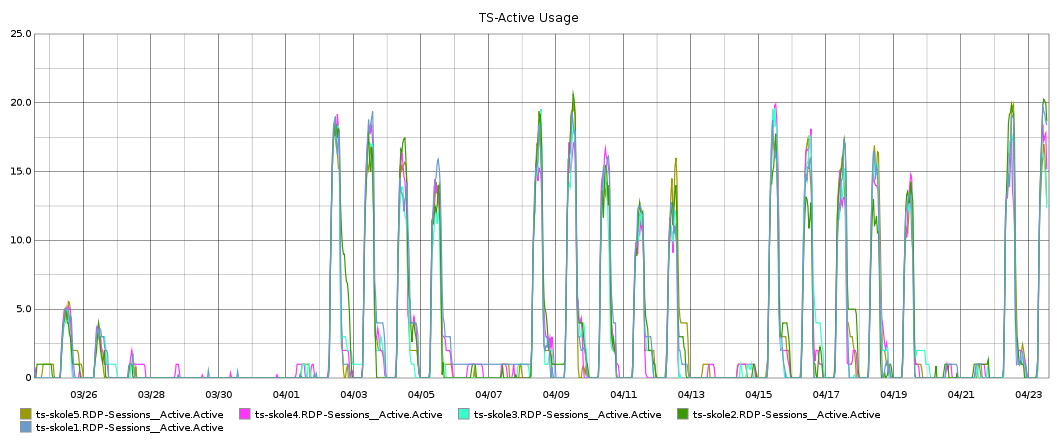
\includegraphics[width=1.0\textwidth]{img/ts-skole-usage-inv}
	\caption{Antall aktive brukere på terminalserverne}
	\label{ts-skole-usage}
\end{figure}

\subsection{Microsoft Exchange}
Microsoft Exchange benyttes som e-postsystem for fylkeskommunen. Her routes og lagres all e-post som sendes ut og inn av alle brukere. I tillegg benyttes funksjonalitet som kalenderdeling, kontakter, og er integrert med telefonsystemet. Exchange er kritisk for kommunikasjon mellom ulike avdelinger i fylkeskommunen, og utad. 

Som for terminalservere, beskrevet i \ref{sec:terminalservere}, brukes Microsoft Performance Monitor for å få tilgang til en rekke viktige tall om Exchange-serverenes ytelse. Firmaet SolarWinds, som selger en kommersiell overvåkningsløsning anbefaler annet at følgende parametre overvåkes\cite{exchange}, i tillegg til basisjekkene CPU, disk og minne:
\begin{itemize*}
	\item Antall tilkoblinger. Dersom antallet er høyt kan det føre til at e-postklienter oppfattes som trege av brukerne.
	\item Gjennomsnittlig responstid på forespørsler. Høye tall vil oppfattes som treghet for brukerne.
	\item Antall meldinger sendt per sekund. Ved høye tall kan det være mistanke om at mail-serveren blir brukt til spam, eller at klienter på nettverket har blitt kompromittert.
	\item Antall LDAP-søk som gir timeout. Høye tall kan indikerer mange tilkoblingsfeil mot Active Directory.
	\item Størrelse på leveringskø. Antall e-poster som ikke har blitt prosessert.
\end{itemize*}
Microsoft har gitt ut egne anbefalinger til grenseverdier som er benyttet som et utgangspunkt\cite{exchangethresholds}.

I tillegg til disse sjekkene var det ønskelig å teste hele e-postoppsettet i én sjekk. Til dette benyttes plugin-en ``check\_email\_delivery'' \cite{exchange}. Her sjekkes det at en e-post kan sendes fra SMTP-serveren. E-posten som sendes ut inneholder en unik ID. Videre kobler plugin-en seg til IMAP-tjenesten og sjekker om e-posten med den unike ID-en kom frem. Antall sekunder for hele round-trip-en blir målt. Helst skulle en sendt e-posten fra en SMTP-server som står utenfor nettverket, men det var ikke tilgjengelig under implementasjonensperioden.

Det sjekkes også at websiden for Outlook Web Access er tilgjengelig, på samme måte som andre websider, slik det er beskrevet i \ref{sec:webservere}.

\subsection{Redundante oppsett}
En ordinær plugin henter status for en service på ett host-objekt. Ved redundante oppsett vil det ikke nødvendigvis være kritisk om en av nodene er nede. For å vurdere statusen til et cluster kan en kjøre en sjekk på hvert enkelt host-objekt, og ta en vurdering basert på resultatene av alle sjekkene samlet.

For å overvåke redundante oppsett, har plugin-ene ``check\_multi'' \cite{checkmulti} og ``check\_cluster'' \cite{checkcluster} blitt vurdert. check\_cluster parser den lokale status.dat-filen og ser hvilken tilstand en service eller en host er ved siste sjekk. Plugin-en check\_multi derimot kjører plugin-er mot spesifiserte host-objekter, og en kan definere sammenligningsoperator (<,>,==), som vil bli sjekket mot de returnerte resultatene.

Med check\_multi kan en benytte en eller flere egendefinerte kommandoer som parametere. Disse vil parses av check\_multi og kan inneholde alt i fra ``echo 'Hello, World!', til mer avanserte Perl-script som kjøres ved hjelp av eval. Dette blir brukt for Oracle-databaser som forklart i \ref{sec:oracle}. 

For å evaluere resultatene fra alle sjekkene samlet, kan en definere kriterier som gir et varsel. Da brukes standard Icinga-tilstander, som vist i eksempelet under:
\begin{lstlisting}[style=example]
command [ HTTP_Node1 ] = check_http -H 192.168.2.10
command [ HTTP_Node2 ] = check_http -H 192.168.2.11
command [ HTTP_Node3 ] = check_http -H 192.168.2.12
command [ HTTP_Node4 ] = check_http -H 192.168.2.13
state [ WARNING ] = COUNT(WARNING) == 2
state [ CRITICAL ] = COUNT(CRITICAL) > 2
\end{lstlisting}
For check\_cluster spesiferes det om det er et host- eller service-cluster som skal sjekkes. Deretter spesifiseres parametere med navn på host og service, og hvor mange host- eller service-objekter som må ha en gitt tilstand, før det varsles WARNING eller CRITICAL. Fordi check\_cluster kjører lokalt på Icinga-serveren, vil den ikke generere noe nettverkstrafikk. Ulempen er at den ikke gir noen informasjon om hvilket host-objekt som er nede eller hvilket host-objekt en service feilet på. Det vil si at den gir bare en overordnet status for det redundante oppsettet. 

Under vises et eksempel for kommandoen check\_cluster som kjører Check HTTP host-objektene localhost, HiG2, HiG3, og HiG4. Det vil bli gitt en WARNING om en av serverene er nede, og CRITICAL om to er nede. 
\begin{lstlisting}[style=example]
./check_cluster --service -l "Check HTTP"  -d $SERVICESTATEID:localhost:Check HTTP$, $SERVICESTATEID:HiG2:Check HTTP$ ,$SERVICESTATEID:HiG4:Check HTTP$  -w @1 -c @2
\end{lstlisting}

\section{Databaser}
Databaser brukes i mange av applikasjonene IKT-avdelingen drifter for brukerne. På databaseserverne samles dataen fra disse applikasjonene på et sted. 
Tre forskjellige databasemotorer brukes. Disse er MySQL, MSSQL og Oracle DB. Hver av disse har ulik arkitektur og virkemåte\cite{databasecomparison}, og derfor blir ikke de samme parameterne overvåket på alle. Felles for alle er:
\begin{itemize*}
	\item Connection time. Tiden det tar å koble til SQL serveren.
	\item Connected users. Antallet aktive sessioner mot SQL serveren.
	\item Cache hit rate. Antallet spørringer som blir hentet fra cache i et tidsintervall.
\end{itemize*}

Noen av sjekkene er spesifikke for hver databasemotor, og er valgt for å få en oversikt over trege spørringer:
\begin{itemize*}
\item MySQL: Slow queries. Antall trege spørringer SQL serveren utfører i et gitt tidsintervall.
\item MSSQL: Lazy writes. Et høyt tall indikerer at mange minne-page-er må skrives til disk. Dette kan indikere mangel på tilgjengelig minne.
\item Oracle: Free table space. Hvor mye ledig plass det er for tabellene.
\item Oracle: Log switch interval. Tid mellom hver gang en ny log opprettes for databasen. Et høyt tall kan indikere høy load på serveren.
\end{itemize*}

\subsection*{Connection time}
Sjekken av connection time tester om det er mulig å koble til SQL-serveren. Hvis denne sjekken gir en timeout, er det fordi sjekken ikke får kontakt på porten til serveren. Det defineres parametere for hvor lang tid det bør ta å koble til. Hvis tilkoblingstiden blir for lang varsler Icinga om dette. Grenseverdier her er valgt ut fra gjennomsnittlig tilkoblingstid over 30 dager.

\subsection*{Connected users}
For connected users sjekkes hvor mange sessioner som er koblet til database tjenesten (per instanse for Oracle DB). Antall aktive sesjoner blir samlet inn om hver enkelt database. Derfor defineres grenseverdier ut fra hvor mange brukere som er koblet til over en periode, og et uvanlig bruksmønster vi gi et varsel.

\subsection*{Cache hit}
Cache hit er hvor ofte data hentes ut fra databasemotorens egen cache, slik at dataen ikke leses fra disk. Dette sparer diskene for I/O-operasjoner. Hvis cache hit ligger på et høyt nivå (90 - 100 \%), indikerer dette at tabellene det spørres mest mot lagres i cache. Når cache hit ligger under 90 \% kan dette være et resultat av at serveren ikke har nok minne til å lagre tabellene i cache. Dette kan indikere et minneproblem.

Oracle mener at cache hit bør ligge på over 90 \% \cite{oraclecachehit}. For MSSQL er tilnærmet 100 \% cache hit et godt utgangspunkt\cite{sqlmonitoring}.

MySQL-databasene til IKT-avdelingen lagrer all databasedata i minnet, så her vil det ikke være relevant å sjekke cache hit. Sjekken er satt opp slik at ordinære MySQL-servere vil kunne settes opp med denne sjekken i ettertid.

\subsection{Forutsetninger for plugin}
For at Icinga-serveren skal kunne snakke med de forskjellige databasemotorene trengs en klient for hver av dem. 

\subsubsection{Oracle}\label{sec:oracle}
Databaseklienten finnes på Oracle sine nettsider\cite{oracleclient}. Den finnes ikke som en deb-pakke, som brukes for Debian. Det finnes derimot en rpm-pakke, som brukes av blant annet Red Hat. Alien ble brukt til å konvertere rpm-pakken over til deb-pakke før installasjon på Icinga-serveren\cite{debian:alien}.

\begin{lstlisting}[style=example]
alien oracle-instantclient11.2-basic-11.2.0.3.0-1.x86_64.rpm 
dpkg -i oracle-instantclient11.2-basic-11.2.0.3.0-1.x86_64.deb
\end{lstlisting}

Videre trengs også en databasedriver, som gjør det mulig for Perl å benytte klienten. For Oracle-databaser brukes ``libdbd-oracle-perl''.

På en Oracle-server vil hver database ha sin egen instans \cite{oraclefaq}. Derfor vil parametere som overvåkes være forskjellig fra instans til instans. Etter utveksling over e-post med utvikler av plugin-en (se e-post i Vedlegg \ref{app:maildb}), og samtaler med ansvarlig for databaser ved IKT-avdelingen ble det avgjort å overvåke hver enkelt databaseinstanse, med plugin-en check\_multi.

Navnene til instansene legges derfor inn som en egendefinert variabel på host-objektet for hver enkelt Oracle-server. Når plugin-en kjøres sjekkes filen tnsnames.ora, som inneholder tilkoblingsinformasjon for hver enkelt instanse, i dette tilfellet må variabelen \_HOSTDBINSTANCES inneholde ORA11. Strukturen for en enkelt instanse vises tnsnames.ora vises under:
\begin{lstlisting}[style=example]
ORA11 =
 (DESCRIPTION = 
   (ADDRESS_LIST =
     (ADDRESS = (PROTOCOL = TCP)(HOST = 127.0.0.1)(PORT = 1521))
   )
 (CONNECT_DATA =
   (SERVICE_NAME = ORA11)
 )
)
\end{lstlisting}

For at Icinga-brukeren skal kunne bruke klienten og finne filen tnsnames.ora kreves det at det brukeren har informasjon om disse i noen miljøvariabler. Dette settes ved å eksportere variablene i ``/etc/sysconfig/icinga'', som kjøres fra init-scriptet til Icinga.
\begin{lstlisting}[style=example]
export ORACLE_HOME=/usr/lib/oracle/11.2/client
export TNS_ADMIN=/usr/lib/oracle/11.2/client/network/admin
\end{lstlisting}

check\_multi brukes for å samle en Oracle-servers instanser under samme service-objekt. For eksempel når cache hit-sjekken kjøres, vil check\_multi utføre sjekken for alle instansene. I webgrensesnittet vil svarene fra instansene samles under ``check cache hit'' for hvert enkelt host-objekt. Dette gjør det mer oversiktlig og dynamisk enn en sjekk for hver instans. Under vises konfigurasjonen for dette.

\begin{lstlisting}[style=example]
define service {
...
    check_command	check_multi!check_oracle! -s dbinstances=$_HOSTDBINSTANCES$ -s host=$HOSTADDRESS$ -s mode=sga-data-buffer-hit-ratio -s warning=93: -s critical=90: -s user=$USER5$ -s pass=$USER4$
}

define command {
...
	command_line	check_multi -r 32 -f /etc/icinga/objects/commands/check_multi/$ARG1$.cmd $ARG2$
}
\end{lstlisting}
%TODO: EXPLAIN
Da check\_multi utfører sin kommando vil ``eeval'' funksjonen sette sammen en kjede med alle instansene som skal sjekkes, for så å kjøre disse separat. Svaret returnert til Icinga vil inneholde status og ytelsesdata for alle instansene i variabelen ``\_HOSTDBINSTANCES''. Det som blir unikt for denne sjekken er at service-objektet vil inneholde status for alle instansene.
\begin{lstlisting}[style=example]
eeval [ oracle_health ] =
    my $chain = "";
    foreach my $instance (split(/,/,'$dbinstances$')) {
        $chain .= "-x \"command[ $instance ] = check_oracle_health --connect '$user$'\/'$pass$'\@'$instance' --mode '$mode$' --warning $warning$ --critical $critical$ \" ";
    }
    parse_lines("command [ check_oracle ] = check_multi -r 4 $chain");
\end{lstlisting}

\subsubsection{MySQL}
For MySQL ligger de nødvendige pakkene i Debians pakkebrønn og kan installeres med apt. De nødvendige pakkene er ``mysql-client'', for databasetilkoblingen og ``libclass-dbi-mysql-perl'', som er en Perl-modul for å kunne koble til en MySQL-server.

\subsubsection{MSSQL}
For MSSQL var det vanskelig å finne en databaseklient som er fri programvare. Det ble etter noe research besluttet å bruke ``FreeTDS''\cite{freetds}, sammen med Perl-modulen ``libdbd-sybase-perl''.

\subsection{Plugin}
Plugin-ene som blir benyttet for databaser er skrevet av firmaet ``Consulting \& Solutions'' og heter ``Check\_MySQL\_Health'', ``Check\_Oracle\_Health'' og ``Check\_MSSQL\_Health''\cite{consol}.

Disse må kompileres fra kildekoden. For å gjøre dette må en først konfigurere de med riktige parametere, før den installeres. Dette er de samme for alle tre plugin-ene.

\begin{lstlisting}[style=example]
./configure --prefix=/usr/lib/nagios/plugins/ --with-nagios-user=nagios --with-nagios-group=nagios --with-perl=/usr/bin/perl --with-statefiles-dir=/tmp
make && make INSTALL
\end{lstlisting}

For å koble til databaseserverne trengs en servicebruker for hver av de. Denne gis minimale tilganger, slik at denne ikke har tilgang til å endre tabeller og spørre etter info. Brukeren vil kun ha tilgang til å kjøre kommandoer for serveradministrasjon\cite{mysqlpriv}.

I MySQL brukes følgende kode for å opprette denne brukeren:
\begin{lstlisting}[language=SQL,style=example]
GRANT USAGE ON *.* TO 'icinga'@'10.60.0.20' IDENTIFIED BY 'Password';
\end{lstlisting}

Script for å opprette brukere i Oracle og MSSQL finnes i Vedlegg \ref{oracledb.sql}.

Konfigurasjon for command-objektet for MSSQL og MySQL vises under. \$ARG1\$ brukes for å sende med hvilken parameter plugin-en sjekker.
\begin{lstlisting}[style=example]
    command_line	$USER1$/check_<database-motor>_health --hostname=$HOSTADDRESS$ --username=$USER5$ --password=$USER4$ --mode $ARG1$ --warning $ARG2$ --critical $ARG3$
\end{lstlisting}

\subsubsection{MySQL Cluster}
MySQL Cluster er et distribuert oppsett for MySQL. Ved IKT-avdelingen benyttes et MySQL Cluster med NDB som lagringsmotor der databasene kjører i minnet. Et MySQL Cluster består av tre forskjellige nodetyper\cite{ndbinformation}:
\begin{itemize*}
	\item \textbf{Management} her konfigureres clusteret og en setter opp hvor mange Data- og SQL-noder som kan kobles til.
	\item \textbf{Data} oppbevarer tabeller og tabelldata i RAM. Disse håndterer lastbalansering, replikering, failover og gjenoppbygging automatisk imellom hverandre.
	\item \textbf{SQL} MySQL-servere som kobler seg til data-nodene for å hente og lagre data.
\end{itemize*}

Den enkleste måten å hente ut statistikk for et MySQL Cluster, er å benytte administrasjonsprogrammet ``ndb\_adm''. Denne kan hentes ut fra installasjonspakken til mysql-cluster\cite{ndbdownload}. I ndb\_adm kan en se hvor mange noder av hver type som er tilkoblet management-noden og minneforbruket til hver av datanodene. De plugin-ene som benyttes baserer seg på output fra ndb\_adm.

Antall noder tilkoblet overvåkes med plugin-en check\_ndbd\cite{ndbnode}. Her ble det gjort en endring i koden slik at serveren som ndb\_adm kobler seg til kan spesifiseres som en parameter.

For minnebruk ble det skrevet en egen plugin (Vedlegg \ref{check_ndb_mem.pl}), da ingen eksisterende plugin ble funnet som tillater å spesifisere hvilke noder som skal sjekkes. ID-ene til nodene som skal sjekkes ble satt opp som en egendefinert variabel i host-konfigurasjonen. Denne sendes til plugin-en via service- og kommando-objektene. Konfigurasjonen for dette er vist under.
\begin{lstlisting}[style=example]
define host {
	...
	_NODEIDS 2,3  ;Data-nodes IDs to check memory usage
}

define command {
	...
	command_line   $USER1$/libexec/check_ndb_mem.pl --host $HOSTADDRESS$ --nodes $ARG1$ --warning $ARG2$ --critical $ARG3$
}
\end{lstlisting}

\section{Applikasjoner}
Muligheten for å se om en applikasjon fungerer slik den skal, er en viktig del av overvåkningen. Det er applikasjonene brukerne benytter seg av og vil sende inn feilmeldinger om. En applikasjons tilstand vil bestemmes av flere service-objekters tilstand. I Icinga benyttes et servicegroup-objekt for å gruppere flere service-objekter.

Et praktisk eksempel på dette vises i Figur \ref{servicegroup_layout}. Her vil applikasjonen ``Web App for ERP'' være avhengig av webserveren for å vise web-grensesnittet til brukerne. En filserver for lesing og lagring av filer, en e-post-server for å sende og motta e-post og en databaseserver som inneholder brukerinfo og andre tabeller. 

\begin{figure}[H]
    \centering
    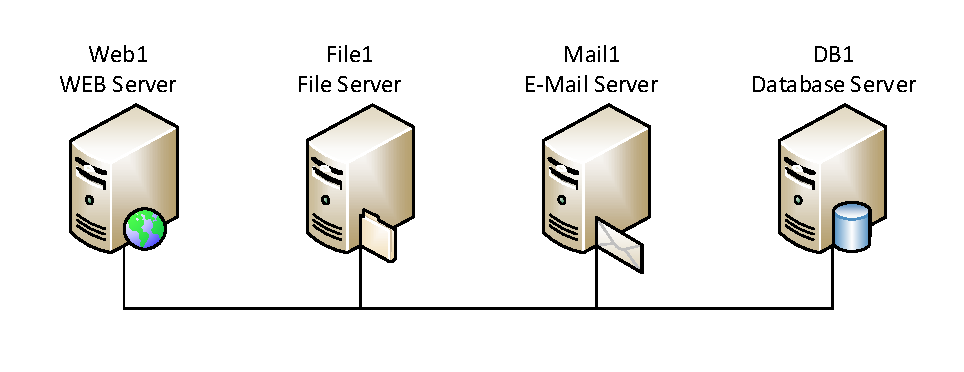
\includegraphics[scale=0.6]{img/servicegroup_layout}
    \caption{Tjenester for servicegroup-objektet ERP\_WEBAPP}
    \label{servicegroup_layout}
\end{figure}

Konfigurasjonen for dette er vist under. Direktivet ``members'' setter medlemmene i gruppen der hvert service-objekt refereres til på formen ``<host\_name>,<service\_description>''.

\begin{lstlisting}[style=example]
define servicegroup {
	servicegroup_name	ERP_WEBAPP
	alias 				Web App for ERP
	members 			Web1,Check ERP Web Contents, File1,Check SMB, Mail1,Check Exchange, DB1,Check MySQL
}
\end{lstlisting}

I dette eksempelet kjøres service-sjekker mot alle tjenestene. Service-objektene grupperes i en servicegroup. Et oversiktsbilde over applikasjonen vises i Icingas web-grensesnitt, som i Figur \ref{servicegroup_web}. Slik blir det enklere for ansatte på servicedesk å kunne gå inn og se hva som er feil med ``Web app for ERP'' om brukere rapporterer om feil på denne applikasjonen.

\begin{figure}[H]
    \centering
    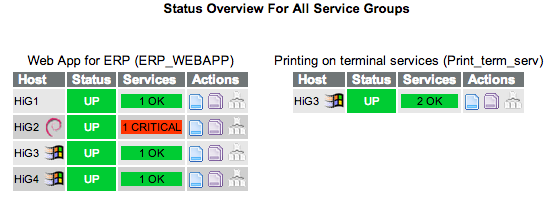
\includegraphics[scale=0.6]{img/servicegroup_web}
    \caption{ Oversikt over servicegroup-objekt og status i webgrensesnittet}
    \label{servicegroup_web}
\end{figure}
Det vil det også være naturlig å sette opp servicedependency-er mellom ``Check ERP Web Contents'' på Web1 og sjekkene for webserveren, filserveren, mailserveren og databaseserveren for å unnga flere varsler ved følgefeil.

\section{Infrastruktur}
Infrastruktur består av de grunnleggende enhetene de andre serverne er avhengig av, og er dermed ekstra viktig å overvåke. I dette prosjektet er det definert til: switcher, routere, brannmurer, UPS, virtualiseringsteknologi og servermiljø.

Det er viktig at design av overvåkningen fører til at man raskt og effektivt skal kunne varsle feil, og hvilke andre enheter dette berører. For å få til dette i Icinga benyttes parent \ref{sec:parent}. De aller fleste enheter i infrastrukturen vil være parent for andre enheter, med unntak av servermiljø. Dette reflekteres også i et statuskart i Icinga, som vist i Figur \ref{statusmap}.

\subsection{Switcher}\label{sec:switch}
Switcher er nettverksutstyr som jobber på lag 2 i OSI-modellen, datalink-laget. IKT-avdelingen benytter switcher som også har lag 3-funksjonalitet. Det vil si at switchen kan kommunisere over IP. Alle switchene IKT-avdelingen benytter støtter SNMP-protokollen, som brukes til overvåkning.

På switchene overvåkes forskjellige sensorer avhengig av hvilke som finnes. Alle switcher har for eksempel ikke vifter. 

Det er laget et generisk oppsett som overvåker temperatur, PSU og viftestatus. Hvilken OID denne informasjonen ligger under varierer fra leverandør til leverandør. For noen produsenter kan denne også være lik. 

Dersom en vifte eller PSU rapporteres som defekt vil det rapporteres som en CRITICAL-status i Icinga. For temperatur blir grenseverdiene hentet ut fra SNMP-objektet ``ciscoEnvMonTemperatureStatusDescr'', der enheten selv rapporterer om temperaturtilstanden er normal, warning eller critical\cite{cisco_env_mib}.

Switchene IKT-Avdelingen bruker er forskjellige modeller fra leverandørne Cisco, Dell og HP. Disse overvåkes med plugin-ene ``check\_nwc\_health'' \cite{checknwc} for Cisco og HP, og check\_snmp\_powerconnect for Dell \cite{checkpowerconnect}.

\subsection{Routere og brannmurer}
IKT-avdelingen benytter Cisco ASA- og Cisco PIX-routere for routing av trafikk mellom forskjellige nettverk. I tillegg utfører de oppgaver som pakkefiltrering, NAT og IPsec-tunnelering for VPN.

\subsubsection{Ressurser}
Plugin-en check\_nwc\_health brukes for å overvåke sensorer, CPU-bruk og minneforbruk.

For CPU-bruk sjekkes gjennomsnittet over 5 minutter. Grenseverdier er satt til 80 \% på WARNING og 90 \% på CRITICAL, i henhold til det Cisco anbefaler \cite{ciscounifiedcommunication}. Høy CPU-bruk kan føre til dårligere ytelse, høy rate av buffer-feil og generelle feil med responsivitet \cite{ciscocpurouters}

I følge Cisco kan høyt minneforbruk under vanlig drift indikere at brannmuren er under angrep\cite{ciscomem}. Dersom en router bruker opp tilgjengelig minne kan det føre til at routeren slutter å svare på kommandoer, telnet-tilkoblinger eller blir mindre responsiv\cite{ciscomemproblem}. Cisco anbefaler en grenseverdi på 15 \% ledig minne\cite{ciscounifiedcommunication}. Grenseverdier for minne er derfor satt til 20 \% for WARNING og 15 \% for CRITICAL.

Begge brannmurene legges i en hostgroup som er lagt på service-objektet for ``cisco\_health'', slik at lokale ressurser sjekkes på samme måte som switcher. Brannmurene legges også inn i en hostgroup som heter Cisco-failover som benyttes i service-objektet for failover.

\subsubsection{Failover}
Cisco-routere og brannmurer har en viktig funksjon som kalles failover. Failover fungerer ved at to like enheter settes opp, der en blir satt som ``primary'' og den andre som ``secondary''. Secondary kan da ta over for primary dersom det skulle bli nødvendig. Routerne kobles sammen med en seriellkabel. Figur \ref{ciscoasafailover} viser denne oppkoblingen. 

\begin{figure}[H]
    \centering
    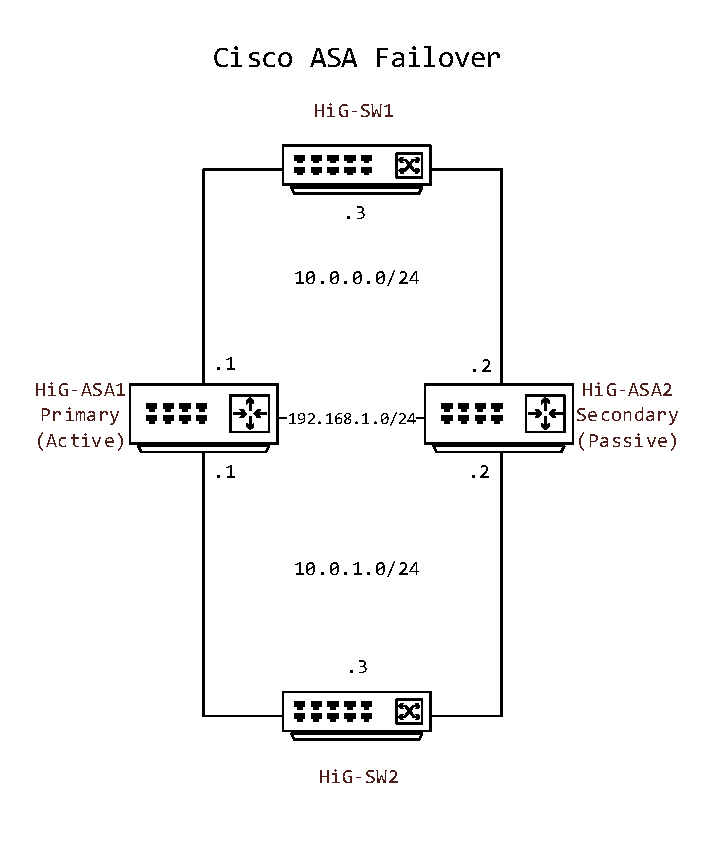
\includegraphics[scale=0.6]{img/asafailover}
    \caption{Oppsett for Cisco-failover}
    \label{ciscoasafailover}
\end{figure}

Dersom secondary mister kontakt med primary, vil secondary ta over nødvendige ruter, brannmurregler og konfigurasjon. Secondary vil dermed overta IP- og MAC-adressen til primary. Primary vil bli satt som passiv (trenger ikke nødvendigvis å ha en IP-adresse på den passive enheten, fordi IP-kommunikasjon kun går gjennom den aktive enheten) helt til en manuelt endrer dette tilbake i konfigurasjonen. \cite{ciscofailover} 

Sjekkene som settes opp for å verifisere at failover-funksjonaliteten fungerer som den skal, og at det ikke har intruffet feil er:
\begin{itemize*}
\item Hvis primary er satt som aktivt og secondary er passiv returneres OK.
\item Om primary er satt som passiv returneres WARNING. 
\item Om secondary er satt som aktiv returneres WARNING.
\item Hvis primary eller secondary får en error returneres CRITICAL.
\item Hvis failover ikke er konfigurert returneres UNKNOWN. 
\end{itemize*}

Til dette benyttes plugin-en ``check\_cisco\_firewall'' \cite{checkciscofirewall}.

Hvis brannmurene deler management-IP på primary og secondary, er det ingen mulighet for å hente ut informasjon fra den passive brannmuren. Da sjekkes failover-status bare for primary. I et ideelt miljø bør både passiv og aktiv enhet ha hver sin IP-adresse, slik at fysiske feil også kan avdekkes på den passive.

\subsubsection{VPN}
For brannmurer som har VPN-tjeneste sjekkes antall oppkoblede brukere opp mot det antallet brannmuren er lisensiert for. Det fantes allerede en plugin som sjekker antall tilkoblede brukere\cite{checkciscovpn}. Plugin-en ble endret til i tillegg å hente ut det maksimale antallet, og sammeligne brukt kapasitet i prosent mot grenseverdier, som kommer inn som argumenter. Plugin-en henter ut variablene over SNMP etter OID-er definert i ``CISCO-FIREWALL-MIB''\cite{cisco_fw_mib}.

\subsubsection{Båndbredde}
For å overvåke bruk av båndbredde inn og ut av en port på Cisco ASA og PIX finnes to muligheter: NetFlow eller hente ut verdien fra en teller i et intervall.

\textit{Netflow}
Funksjonen Netflow\cite{ciscoiosnetflow} fungerer ved at enheten samler inn informasjon og statistikk om alle pakker som går inn og ut av portene. Dette krevet at Netflow konfigureres på alle routerne, og det vil også ta opp ekstra minne og CPU\cite{cisconetflowperf}. Det ble derfor avgjort at Netflow ikke skulle benyttes.

\textit{Telle pakker}
Både Cisco Pix og ASA har tellere for antall byte som går ut og inn på en nettverksport. For å kalkulere bruk av båndbredde over et intervall kan en hente ut disse, vente en gitt periode og hente ut nye verdier. Da vil bruken være ((målepunkt2 - målepunkt1)*8) / antall sekunder.

Mange plugin-er benytter seg av dette ved å lese ut ``ifInOctets'' og ``ifOutOctets'' over SNMP. Dette følger Ciscos notat ``How to Calculate Bandwidth Using SNMP''\cite{ciscobandwidth}. 

En stor ulempe med å benytte disse er at de er 32 bit, og vil dermed nullstilles kjapt ved høye hastigheter. For 1000 Mbps vil det ta ca. 34 sekunder til telleren har brukt opp tilgjengelig bit og nullstilles. Se Tabell \ref{kalkulering_teller} for andre hastigheter.
\[\frac{(2^{32}-1)\:B}{\frac{10^9\:b/s}{8\:b/B}}=34.36\:s \] 
Det er derfor anbefalt å bruke 64 bit-variablene ifHCOutOctets og ifHCInOctets i stedet for\cite{ciscosnmpcounters}.
\begin{table}
\begin{center}
\begin{tabular}{ | l | p{7cm} |} \hline
    \textbf{Hastighet} & \textbf{Tid} \\ \hline
    10 Mbps & 57 minutter og 15.97 sekunder \\ \hline
    100 Mbps & 5 minutter og 43.60 sekunder \\ \hline
    1000 Mbps & 34.36 sekunder \\ \hline
\end{tabular}
\caption{Sekunder før en 32 bit teller nullstilles }
\label{kalkulering_teller}
\end{center}
\end{table}
Plugin-en det er tatt utgangspunkt i for å hente ut båndbreddebruk heter ``check\_iftraffic64\cite{checkciscoif}''. Denne er noe omskrevet for å kunne sende inn absolutte verdier som grenseverdier for varsling. I template-en ``generic\_firewall'' er det satt opp to egendefinerte variabler, ``WANWARN'' og ``WANCRIT'', som setter standard grenseverdier for alle brannmurer. For brannmurer der det er normalt med høyere båndbreddebruk, er disse variablene overstyrt i konfigurasjonen for host-objektet.

\subsection{VMware og Citrix Xen}
Ved IKT-avdelingen benyttes virtualserings-teknologier levert av VMware og Citrix. VMware vSphere 5.1 og Citrix XenServer 6.1 benyttes som virtualserings-platformer, og har funksjonalitet som kreves for en virtualisert infrastruktur. På de fysiske serverene kjører hypervisorene VMware ESX 4.1 og Xen 6.1. Hypervisorene står for kjøring av virtuelle maskiner og virtualiserer ressurser som cpu, minne, disk, og nettverkskomponenter. De virtuelle maskinene kjører operativsystemene og applikasjoner brukere benytter seg av.  

Overvåkning av host-ene som kjører hypervisorene vil bestå av CPU-bruk, minnebruk, I/O, nettverkskomponenter og helsetilstand.

For overvåkning av virtuelle maskiner innenfor begge plaformene brukes NRPE. Det overvåkes da som en ``egen'' server. Ressurser som overvåkes er gjennomgått i \ref{sec:lokaleressurser}.

\subsubsection{VMware}
I VMware vSphere brukes begrepene ``Datacenter'', ``Cluster'', ``Host'', og ``Virtual Machines'', og hver av disse har informasjon tilgjengelig for uthenting. 

\paragraph{Plugin}
Plugin-en ``check\_vmware\_api.pl'' , som er utviklet av fri programvare firmaet op5 \cite{op5}, er brukt for å hente ut informasjonen fra VMware VirtualCenter. Denne plugin-en bruker et SDK-bibliotek i Perl \cite{vmwareperl} for å utføre API-kall til VirtualCenter. Autentisering skjer ved å sende med brukernavn og passord for en brukerkonto, som er opprettet i Virtual Center-serveren med read-rettigheter. For å utveksle informasjon blir SOAP-protokollen benyttet \cite{wiki:soap} via HTTPS \cite{ciscovirtual}.

check\_vmware\_api.pl har mulighet for å hente ut informasjon fra komponenten Datacenter, Cluster, Host, og VM. For hver er informasjon som cpu, minne, I/O, nettverkstrafikk, lagring, og helsetilstand tilgjengelig.

Data blir hentet ut i fra VMware Virtual Center, og her brukes fire intervaller for lagring av historisk data \cite{vmwareperf}. Dette er gjennomsnittet for:
\begin{enumerate*}
        \item hvert 5. minutt for en dag
        \item hvert 30. minutt den siste uken
        \item hver 2. time den siste måneden
        \item hver dag det siste året
\end{enumerate*}

Eksempel på bruk av check\_vmware\_api.pl for å hente ut cpu-bruk for en Host
\begin{lstlisting}[style=example]
./check_vmware_api.pl -D vc.example.org -u user1 -p password123 -H Example-ESX01 -l cpu -s usage -i 300 -T 600
\end{lstlisting}

Med opsjonen ``-i'' spesifiseres intervallet en gjennomsnittsverdi skal returneres fra (første intervall i dette tilfellet). Dette gjennomsnittet baserer seg på datapunkter samlet inn for hvert 20. sekund av VMware VirtualCenter. Opsjonen ``-T''  er ``timeshift'' i sekunder, som kan brukes for å spesifisere tidsintervallet gjennmomsnittsverdier skal returneres fra. 

For de parametere som blir overvåket blir tilleggsopsjonene ``-i 300'' og ``-T 600'' sendt med. Etter gjennomgang av output fra plugin-en ble det observert at dette var innstillingene som ga oss gjennomsnittet for det siste 5 minutters-intervallet. Ved bruk av for eksempel ``-T 60'', som vil si at vi spør 1 minutt tilbake i tid, ble det ikke alltid returnert et resultat siden det ikke har blitt lagret et gjennomsnitt for et 5. minutters intervall i denne perioden. 

Andre opsjoner som ble testet før kombinasjonen ``-i 300'' og ``-T 600'' var``-i 300'', men her kom det 288 resultater tilbake. Dette er antall datapunkt som blir generert i 5 minutters-intervallet for en dag. (86400 / 300)
\paragraph{Ressurser}
Ressurser som overvåkes nå er CPU-bruk, minne-bruk, I/O responsitivitet, status for nettverkskort, og generell helsestatus som rapporteres fra VirtualCenter.\cite{ciscovirtual} \cite{vmwaremonitoring}:

\subsubsection*{CPU}
Grenseverdier her er satt til samme nivå som tilsvarende alarm i VirtualCenter, og kan gi en indikasjon på at CPU-kraften ikke strekker til for en eller flere virtuelle maskinenr. Dette kan føre til at virtuelle maskiner ikke får kjørt tid på de fysiske CPU-ene og går utover eksekvering av prosesser.  \cite{vmwarecounters}.

Teller som blir sjekket er usage.average (\%). Dette er aktiv bruk av CPU i prosent iforhold til total tilgjengelig CPU-kraft. Kalkuleringen her er antall CPU-er ganget med klokkefrekvens.

Grenseverdier (\%): WARNING 75, CRITICAL 90

\subsubsection*{Minne}
Grenseverdier for minne er satt til samme nivå som tilsvarende alarmer i VirtualCenter, og vil gi indikasjon på om virtuelle maskiner krever mer minne enn hosten har tilgjengelig. Når ledig minne går under 6 \%(tilgjengelig), kan host-en iverksette swapping. Når host-en starter å swappe vil den ikke ta hensyn til hva den henter av minne fra de virtuelle maskinene. Dette kan gå utover funksjonalitet og applikasjoner som den virtuelle maskinene kjører.

Counter: usage.average (\%). Dette er en prosentandel av konsumert minne iforhold til totalt tilgjengelig fysisk minne.

Grenseverdier (\%): WARNING 80, CRITICAL 90

\subsection*{I/O}

Overvåkning av tid brukt på I/O operasjoner kan avdekke ytelsesproblem mellom host og virtuelle maskiner, og mellom host og lagringsenheter benyttet. Uthenting av informasjon her er foreløbig bare sanntidsdata når sjekken kjører. Counters hentet ut for I/O, aggregeres ikke ved standard innstilling for lagring av data i VMware VirtualCenter. Standard innstilling er ``level 1``, og det kreves ``level 2'' for å kunne benytte disse counter-ene.

Flere anbefalinger eksisterer for overvåkning av I/O counters, men disse baseres på real-time data, og VMware anbefaler at det ikke overstiger 10ms over en periode. Opsjonene ``-i 300'' og ``-T 600'' kan benyttes etter aktivering av level 2 for aggregering av data.

Counters for I/O:

{\bf disk.kernelLatency.average} - Tiden i millisekunder hver SCSI-kommando bruker fra virtuelle maskiner til den fysiske kontrolleren på host-en. Denne inkluderer også hvor mye tid hver kommando bruker i kø før den blir prossesert, og kan indikere et høyere antall diskforespørsler enn host-en eller den fysiske kontrolleren takler.
 
{\bf disk.deviceLatency.average} - Tiden det tar å fullføre en SCSI kommando mellom den fysiske kontrolleren og lagringsenheten benyttet. Dette kan gi indikasjon på ytelsesproblemer for lagringsenheten, eller den fysiske kontrolleren. 

Videre overvåkes det totale antallet av kernelLatency og deviceLatency for både skrive- og lese-operasjoner, og disse kan indikerer hvilke diskoperasjoner som skaper ytelsesproblemer. Ved høye tall kan en benytte de to over for å se hvor i systemet ytelsesproblemene befinner seg. 

{\bf disk.totalReadLatency.average} - Total tid samlet i millisekunder for kernelLatency og deviceLatency for skrive-operasjoner. 

{\bf disk.totalWriteLatency.average} - Total tid samlet i millisekunder for kernelLatency og deviceLatency for lese-operasjoner.

I tillegg til de over kjøres det to sjekker som gjenspeiler status fra VirtualCenter. Disse er nettverskort som sjekkes om de er OK, og en generell helsetilstand. H

Bruk av NRPE for host-er kan være aktuelt om en vil forsikre seg om at det lagres data om cpu, minne, og diskplass skulle vCenter gå ned. All informasjon om hosts avhenger nå av at VirtualCenter-serveren kjører, og er et ``single point of failure''.

For kapasitetsmåling og helsestilstanden for et cluster kan det settes sjekker for cpu, minnne og helsetilstanden rapportert fra VirtualCenter. En bruker da opsjonen ``-C'' med navn på cluster tilsvarende ``-H''

\subsubsection{Citrix Xen}
I motsetning til VMware der all informasjon kan hentes ut fra ett punkt (VMware VirtualCenter), må en for Citrix Xen  kontakte en master-host for et gitt cluster. Master-hosten har ansvar for å presentere et administrativt grensesnitt, og videresender kommandoer mot spesifikke hosts i clusteret.

\paragraph{Plugin}
For overvåkning av Xen-miljøet ble det kun funnet én plugin som gir muligheten for å hente ut informasjon fra host-er og virtuelle maskiner. Plugin-en ``check\_xen\_api.pl'' bruker biblioteket ``XenAPI'' for å generere URL-er. Disse brukes videre for spørringer mot en RRD-database, hvor ``XAPI'' lagrer data\cite{xenwiki}. Det er ikke like mange tellere som er tilgjengelige som for VMware og I/O-data er foreløpig ikke tilgjengelig for hosts. Ressurser som er satt for overvåkning på host-er er CPU- og minnebruk.

RRD-databasen check\_xenapi.pl spør, lagrer data i følgende intervaller:
\begin{enumerate*}
        \item Hvert 5. sekund i en 10 minutters periode
        \item Hvert minutt for de siste 2 timene
        \item Hver time for den siste uken
        \item Hver dag for det siste året
\end{enumerate*}

For hvert 5. sekund blir aktuelle datapunkter lagret. For de andre intervallene blir en minimum-, maksimum-, og gjennomsnittsverdi over gitt tidsperiode lagret ved bruk av en konsolideringsfunksjon. \cite{xenrrd}


Et eksempel på bruk av check\_xenapi.pl: 
\begin{lstlisting}[style=example]
./check_xenapi.pl -S 10.0.1.50 -u xenuser1 -p password -H XEN_HOST-01 -l cpu -s usage -i 300
\end{lstlisting}

Opsjonen ``-H'' brukes for å spesifisere hvilken host en vil kjøre sjekken mot. Den må være i samme cluster som oppgitt master-host i opsjonen ``-S''. Opsjonen ``-i'' spesifiserer over hvor mange sekunder en skal hente ut data. Resultatet blir da et gjennomsnitt for gitt tidsperiode, og er tilgjengelig for CPU- og minnebruk for hosts.

Som en ser fra eksempelet må det angis addressen til to enheter for å hente ut informasjon, master host-en og host-en en vil ha informasjon om. For å kunne sette en master-IP på ett ojekt, og ikke for hvert host-objekt i et cluster, ble det opprettet et generic-objekt. I generic-objektet settes master IP-en til et gitt cluster via en customvariable. Alle host-objekter som bruker dette generic-objektet arver da denne customvariabelen, og master IP-en kan endres fra et punkt.

Under vises et eksempel hvordan dette kan konfigureres for ett pool med to host-objekter:
\begin{lstlisting}[style=example]
// generic-objektet 
define host {
    use 		generic_linux_host
    name 		generic_xen_pool_1
    _MASTERIP 		10.0.1.50
}

// To host-objekt som arver generic-objektet
define host {
    name 		Cluster_1_Xen_Host_1
    address 		10.0.1.51
    use 		generic_xen_cluster_1
}

define host {
    name 		Cluster_1_Xen_Host_2
    address 		10.0.1.52
    use 		generic_xen_cluster_1
}
\end{lstlisting}

Opsjenene blir da ``-S \$HOST\_MASTERIP\$'' og ``-H \$HOSTADDRESS\$''.

Det oppstod et problem under implementeringen av check\_xenplugin.api, som hadde innvirkning på returnert resultat fra RRD-databasen. Etter å ha lest gjennom koden til selve plugin-en og biblioteket XenAPI som også er skrevet av op5, ble det oppdaget at denne plugin-en bruker siste datapunkt fra intervall nr.1 nevnt over. Resultatet vil da bare være ett datapunkt. Dette er vanskelig å sette varsel på, da en spike kan skje når gitt sjekk kjører. Her ble det avgjort å legge til en ny opsjon for å angi over hvor lang tidsperiode en skal hente ut data. Returnert resultat fra gitt tidsperiode blir gått gjennom, og en gjennomsnittsverdi returneres. Dette er foreløpig bare implementert for CPU- og minnebruk for en host


\paragraph{Ressurser}
Ressurser som er valgt å overvåke for Xen hosts:
\begin{itemize*}
        \item CPU-bruk i prosent (totalbruk for alle kjerner ÷ antall kjerner)
        \begin{itemize*}
                \item Grenseverdier (\%): WARNING 80, CRITICAL 90
        \end{itemize*}
        \item Minne-bruk (Totalt allokert minne - ledig minne)
        \begin{itemize*}
                \item Grenseverdier (\%): WARNING 80, CRITICAL 90
        \end{itemize*}
\end{itemize*}

Det må gjøres endringer i check\_xenapi.pl for å få korrekt returnerte data, og dette er bare implementer for CPU-bruk og minne for en host slik det står nå.For å minske administrative oppgaver rundt overvåkning av Citrix Xen kan det være aktuelt i ta i bruk check\_nrpe for å hente ut informajson om de lokale ressursene. Plugin-en kan derimot brukes for å hente ut informasjon som I/O om virtuelle maskiner, men plugin-en må altså modifiseres til å kalkulere gjennomsnittsbruk.

\subsection{Trådløse kontrollere}
IKT-avdelingen bruker en kontrollerløsning fra Meru Networks på trådløse nettverk. Disse har en viktig rolle i fylkeskommunens nettverk. På en dag har disse rundt 6000 samtidige brukere tilkoblet via aksesspunkter ute på hver lokasjon.

Aksesspunktene inneholder ingen konfigurasjon da de starter opp, denne lastes fra kontrolleren. Alle tilkoblingene går i krypterte sesjoner direkte mot kontrolleren hvor trafikken blir sendt til respektive mottakere. Fordi det går store mengder trafikk over de trådløse nettverkene er det viktig at kontrollerne blir overvåket.

De trådløse kontrollerne mangler støtte for SNMP-get for informasjon som hentes ut fra switcher og brannmurer, som CPU- og minnebruk. Dette vil i følge produsenten komme i en senere firmware-oppdatering. Noe av dette kan løses ved å bruke SNMP-traps i stedet og definere verdier for når disse skal sendes ut direkte på kontrollerne. Her ble relevante trap-meldinger som omhandler kontrollerne satt opp:
\begin{itemize*}
	\item Hardware-feil på kontrolleren.
	\item Ressursmangel på kontrolleren.
	\item Rogue AP. Et udefinert aksesspunkt er oppdaget av de andre aksesspunktene.
	\item Failover til annen kontroller.
	\item Feil på tilkobling mot Radius.
	\item Lisens utløpt.
\end{itemize*}

For å få til dette trengs et mellomledd som kan motta SNMP-traps på Icinga-serveren, tolke trap-meldingene og sende informasjonen videre til Icinga. 

For å lytte etter SNMP-traps benyttes SNMPtrapd\cite{snmptraps2}. Her mottas alle trap-meldinger som sendes med riktig community string. Disse sendes så videre til snmptt (SNMP Trap Translator\cite{traptranselator}). Her defineres de trap-meldingene en er ute etter, informasjon om OID-ene og kommandoen som skal kjøres når denne mottas. I Figur \ref{snmptrap} illustreres hvordan en trap blir prosessert. 

\begin{figure}[H]
    \centering
    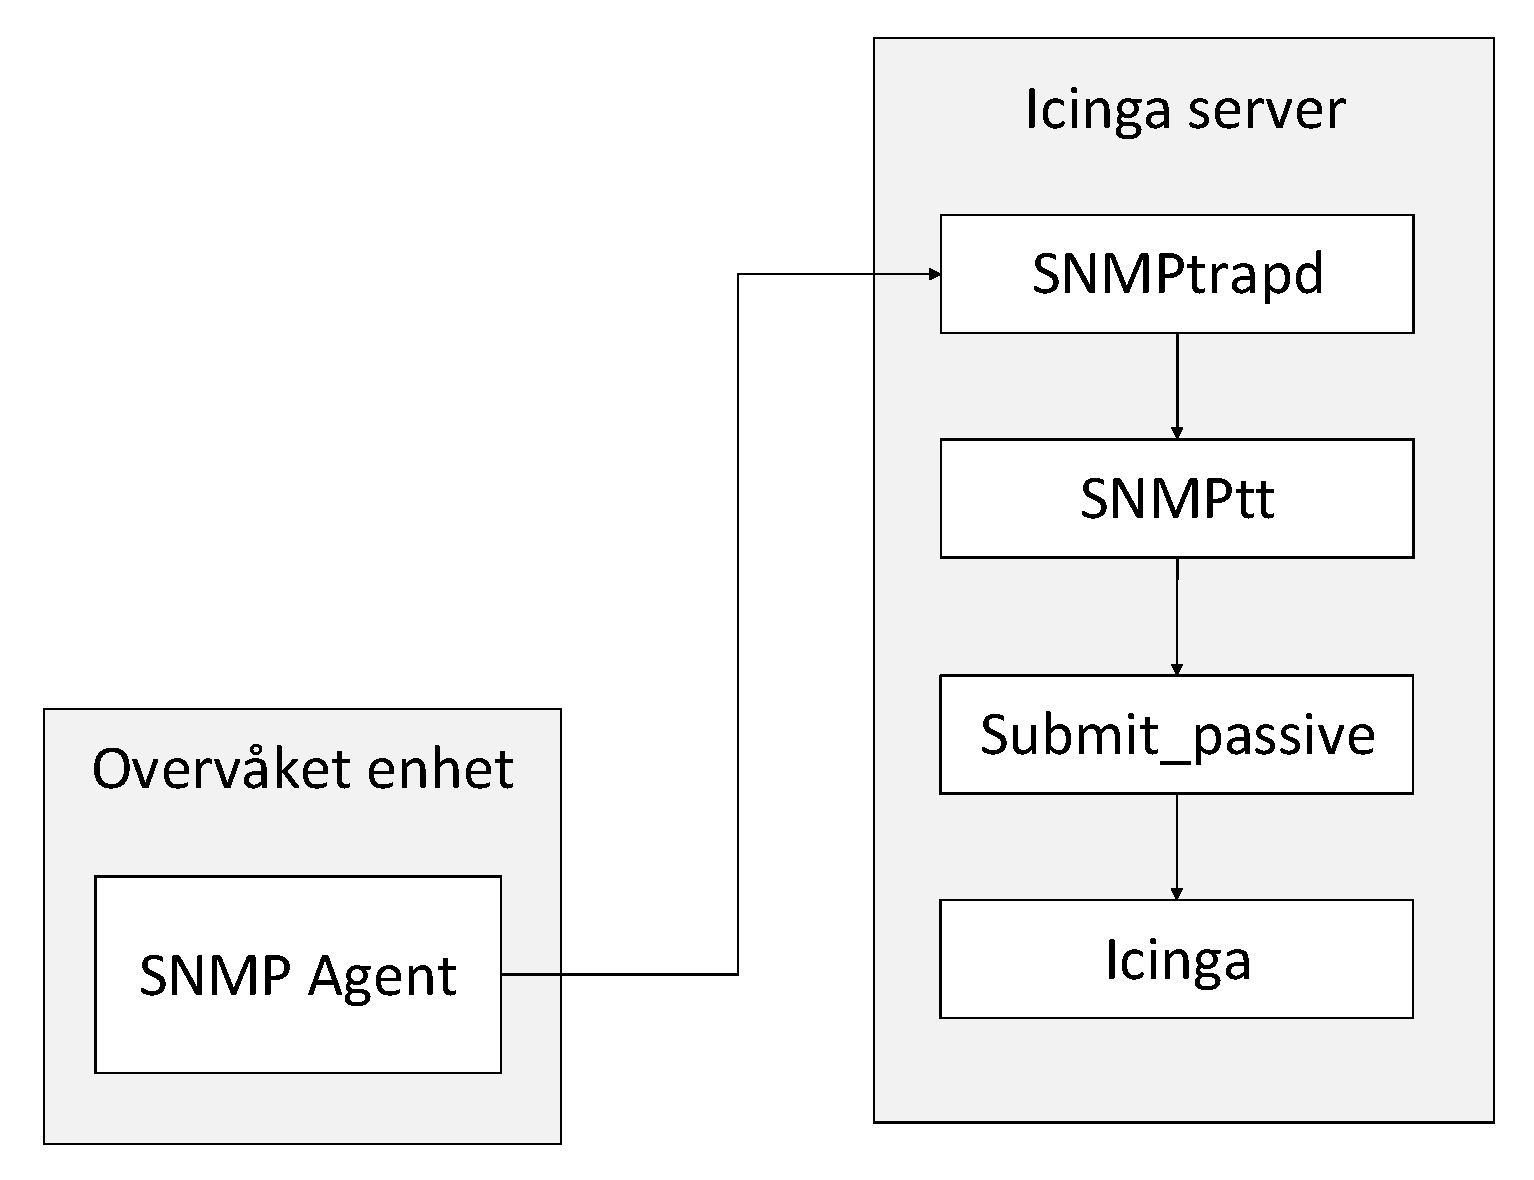
\includegraphics[scale=0.4]{img/SNMPtrap}
    \caption{Trap-prosessering}
    \label{snmptrap}
\end{figure}

SNMPtt trenger konfigurasjon for alle OID-ene som skal prosesseres. Disse kan opprettes med snmpttconvertmib ut i fra en MIB-fil slik:
\begin{lstlisting}[style=example]
snmpttconvertmib --in=MERU-WLAN-MIB.my --out=meru.conf --exec='/usr/lib/nagios/plugins/libexec/submit_check_result "$aA meru_$N 2 $D"
\end{lstlisting}

Eksempel på en OID som blir generert i filen meru.conf:
\begin{lstlisting}[style=example]
EVENT mwlRogueApDetected .1.3.6.1.4.1.15983.3.1.3.13 "Status Events" Normal
FORMAT $*
EXEC /usr/lib/nagios/plugins/libexec/submit_check_result $aA meru_$N 2 "$D"
SDESC
A rogue AP is detected. The AP id, mac address, and other information are described in mwlTraContent.
EDESC
\end{lstlisting}

Her benyttes variabler i snmptt\cite{snmptrans}:
\begin{itemize*}
	\item IP-adressen til SNMP-agenten, altså kontrollereren
	\item Navnet på trap-en
	\item Beskrivelse på trap fra konfigurasjonfilen.
\end{itemize*}

SNMPtt vil så kjøre kommandoen definert under ``EXEC'' for OID-en, som i dette tilfellet er å sende informasjonen videre til scriptet ``submit\_check\_result''. Dette tar fire argumenter:

\begin{itemize*}
	\item IP-adresse eller hostname 
	\item Service description
	\item Returkode som setter tilstand på service-objektet (0-3)
	\item Plugin-output
\end{itemize*}
Scriptet skriver dette sammen med et timestamp til icinga.cmd som Icinga sjekker periodisk etter resultat av passive sjekker.

Service description for alle meru traps som sendes inn vil da være ``meru\_'' + navnet på trap-en. Som plugin-output er det lagt inn beskrivelse av trap-en, da denne som regel er noe mindre kryptisk enn navnet.

Noe å merke seg er at en ikke vil få informasjon når tjenesten er OK igjen, og må sette tjenestene til OK manuelt i Icingas webgrensesnitt.

\subsection{Servermiljø}
For å overvåke temperatur og luftfuktighet på serverrommet ble det kjøpt inn en APC NetBotz 200 med fire eksterne sensorer. Disse ble plassert slik at det er to sensorer på hver side av rack-raden. En vil dermed kunne se temperaturforskjellen mellom forsiden av serverne, ved luftinntak og baksiden, der varmluft går ut.

Hver sensor måler både temperatur og relativ luftfuktighet.

\subsubsection{Luftfuktighet}
Relativ luftfuktighet er definert som ``forholdet mellom partielltrykket til vanndamp, i en gassblanding av luft og vann, og vanndampens metningstrykk ved en viss temperatur''. Dette gir en prosentandelen av vann i luften\cite{wiki:luftfuktighet}. 

Mange enheter for overvåkning av servermiljø måler også duggpunkt. Et duggpunkt er temperaturen en viss mengde luft må avkjøles til for at vanndamp skal kondensere. Ved en økning i relativ luftfuktighet vil duggpunktet nærme seg luftemperaturen. Ved 100 \% relativ luftfuktighet vil temperaturen og duggpunktet ha samme verdi. 

I ``Sun Microsystems Data Center Site Planning Guide'' anbefales en luftfuktighet på 45 - 50 \%. Det meste av datautstyr kan fungere innenfor et bredere intervall enn det, typisk 20 - 80 \%. Men de anbefalte verdiene er satt for at det skal være et buffer dersom en har klimaanlegg som kontrollerer luftfuktighet, og det slutter å fungere\cite{planningserver}. Andre, som ``American Society of Heating, Refrigerating and Air-Conditioning Engineers'' (ASHRAE) anbefaler at den relative luftfuktigheten ikke bør overstige 60 \%, mens den nedre grensen er basert på duggpunkt og satt til 5.5° C, der den relative luftfuktigheten vil variere mellom 25 og 45 \% \cite{envguide}. Disse verdiene er også anbefalt av Cisco\cite{envguidecisco}, og omtalt som vidt akseptert. 

Høy luftfuktighet kan føre til kondens, som igjen kan føre til korrosjon på komponenter. Ved lavere luftfuktighet øker faren for utladninger av statisk elektrisitet (kritisk ved 30 \%), som kan føre til utladninger med ekstremt høye spenningsverdier. Dette kan ødelegge komponenter.

\subsubsection{Temperatur}
Det er mye uenighet rundt anbefalte verdier for temperatur i serverrom. I et studie utført ved University of Toronto\cite{torontopaper}, ble det samlet inn data fra tre forskjellige organisasjoners datasentre, deriblant Googles. I studiet ble det konkludert med at faren for hardware-feil ved høyere temperatur øker mindre enn det som har vært vanlig å basere seg på. For DRAM-feil og servere som stopper momentant fant de ingen korrelasjon til temperaturøkning for intervallet i testen (15 - 60 °C). I dette studiet ble det ikke målt eller tatt hensyn til luftfuktighet. 

ASHRAE anbefaler en inntakstemperatur 18 - 27 °C, mens Suns anbefaling er 20 - 23 °C. Sun begrunner sin anbefaling med at det er lettere å opprettholde trygge verdier for relativ luftfuktighet med dette temperatur-intervallet. ASHRAE refererer også til studier som viser at det totale strømforbruket kan gå opp ved høyere temperaturer, fordi enheter øker frekvensen på egne vifter\cite{datacentertemp}.

\subsubsection{Plugin for overvåkning av temperatur og luftfuktighet i Icinga}
Det fantes allerede en plugin for å sjekke sensorverdiene på APC NetBotz\cite{checknetbotz}, men denne sammenlignet verdiene med grenseverdier satt i konfigurasjonen på enheten. Det var ønskelig å samle mest mulig av konfigurasjon på Icinga-serveren, derfor ble plugin-en omskrevet til å kunne ta inn øvre og nedre grenseverdier som argumenter.

\subsection{UPS}
UPS (Uninterruptible Power Supply), ofte kalt avbruddsfri strømforsyning på norsk, blir benyttet til å opprettholde strøm til alle enheter på IKT-avdelingens serverrom dersom strømnettet skulle falle ut. Strømmen filtreres også slik at utstyr ikke vil bli skadet av overspenning. Ved IKT-avdelingen benyttes UPS-er av fabrikatene APC og HP.

For HP og APC overvåkes:
\begin{itemize*}
 	\item Gjenstående batterikapasitet.
	\item Prosentandel belastning.
	\item Spenning inn og ut.
\end{itemize*}
På APC UPS-er overvåkes også intern temperatur. For både HP og APC overvåkes alle parametere direkte over SNMP med plugin-en ``check\_snmp'' fra nagios-plugins. Her er OID-ene definert direkte i service-objektene.

Under vises et eksempel på hvordan inntaksspenning overvåkes på en APC UPS:
\begin{lstlisting}[style=example]
./check_snmp -H $HOSTADDRESS$ -C <community string>-o .1.3.6.1.4.1.318.1.1.1.3.2.1.0 -l "Voltage In" -w 225:239 -c 220:245 -u "V"
\end{lstlisting}

\subsubsection{Varsling}
Varsling er en funksjon i overvåkningsløsningen som krever en del finjusteringer og balansering av parametere over tid. Det vil være en balansegang med å varsle for mye og filtrere for grovkornet. Et tegn på et godt overvåknsingssystem er at det er fokusert, og ikke gir oveflødig mengde informasjon /cite  Building a Monitoring Infrastructure with Nagios . Dersom det ofte sendes ut “falske varsler” kan dette føre til at en alvorlig hendelse ikke blir oppdaget selv om det faktisk sendes ut varsel. Når varsler sendes ut er det til de som vil og trenger å få de.

\subsubsection{Avhengigheter}
For å holde antallet varsler som sendes ut nede benyttes avhengigheter som beskrevet i \ref{sec:servicedependency}  og \ref{sec:parent} for å ikke få mer enn en melding ved følgefeil. “Parent” har blitt benyttet til å reflektere det fysiske nettverksoppsettet. Service dependency-objekter er satt opp for noen tjenester. For eksempel tjenester som blir sjekket via NRPE vil være avhengig av at NRPE-daemonen på gitt host kan motta henvendelser.

\subsubsection{Konfigurasjon}
I Icinga kan man lage kontakter og legge disse i kontaktgrupper. Oppsettet følger samme logikk som at et hostgroup-objekt referer til en eller flere host-objekt i et service-objekt.
Det vil si at contact- og contactgroup-objekter refereres til i et service- eller host-objekt. Disse kontaktene kan bli varslet om service-objektet får en annen status enn OK. Dette konfigureres i service-objektet sammen ved hvilke tilstander som skal varsles. Disse tilstandene er vist i tabell \ref{notications}.

Når en feil oppstår vil Icinga vurdere ulike konfigurasjonsopsjoner før det eventuelt sendes ut et varsel. Om konfigurasjonsopsjonene tilsier at det skal varsles, vil Icinga gå igjennom filtre som er ferdig definert, som for eksempel om kontakten eller gruppen skal ha varsel via sms eller email. 

\begin{table}
\begin{center}
\begin{tabular}{| c | l | l | p{7cm} |}
        \hline
        \textbf{Objekt} & \textbf{Opsjon} & \textbf{Tilstand} & \textbf{Det sendes varsler om}
        \\ \hline
	\multirow{3}{*}{Host} & d & DOWN 			& Host-objektet er nede 			\\ \cline{2-4}
					    & u & UNREACHABLE 		& Et parent er nede eller unreachable.		\\ \cline{2-4}	
					    & r & UP 			& Hosten går til UP				\\ \hline 
        \multirow{3}{*}{Service} 	    & c & CRITICAL 		& Service-en er i CRITICAL 			\\ \cline{2-4}
					    & w & WARNING  		& Service-en er i WARNING  			\\ \cline{2-4}
					    & u & UNKNOWN  		& Service-en er i UNKNOWN  			\\ \hline
	\multirow{4}{*}{Host eller Service} & f & FLAPPING           	& Flapping starter eller slutter 		\\ \cline{2-4}
					    & s & Scheduled downtime 	& Planlagt nedetid starter eller slutter 	\\ \cline{2-4}
				 	    & r & UP                 	& Objektet går til UP 				\\ \cline{2-4}  
					    & n &                    	& Det skal ikke varsles ved noen tilfeller 	\\ \cline{2-4}

	\hline
\end{tabular}
\label{objekt_varsling}
\end{center}
\end{table}


\subsubsection{Flapping}
I Icinga defineres “flapping” som når et host- eller service-objekt skifter tilstand for ofte, noe som resulterer i mange problem- og recoveryvarsler. \cite{icingaflapping} Dersom detektering av flapping er konfigurert for objektet vil Icinga stoppe varsler for det dersom prosentandelen flapping overstiger en konfigurert grense. Objektet regnes som å ha startet å flappe når andelen for første gang overstiger en “høy”-grense og som å stoppe å flappe når andelen igjen er under en “lav”-grense.

Denne prosentandelen er kalkulert ved at
\begin{itemize}
	\item Lagrer resultatet for de siste 21 sjekkene.
	\item Finner når tilstandsendring skjer 
	\item Kalkulerer flap prosent ut fra andelen tilstandsendringer
	\item Vekter nyeste sjekker mer
\end{itemize}

Som standard er denne grensen satt til 20.0 for høy og 5 for lav i Icinga.cfg. Men den kan også konfigureres på hvert host- og service-objekt med direktivene “low\_flap\_threshold” og “high\_flap\_threshold”, som vist i eksempelet under:

\begin{lstlisting}
define host {
	name important_servers  		#template
	use generic_host
	flap_detection_enabled          1     ; Flap detection is enabled
	low_flap_threshold		70    ; Stop flapping at 70 %
	high_flap_threshold		80    ; Start flapping at 80 %
	register			0
}
\end{lstlisting}

\subsubsection{Oppsett av kontakter og kontaktgrupper}


IKT-avdelingen ønsket å kunne styre kontaktinformasjon og kontaktgrupper fra Active Directory. Det ble bestemt at ansvarsforhold skulle gjenspeiles i kontaktgrupper /ref vedlegg møte, for eksempel “ts\_ansvarlig” eller “printer\_ansvarlig”. Icinga støtter ikke integrasjon mot LDAP i konfigurasjonsfilene, men siden disse er rene tekstfiler kan de enkelt opprettes og endres med script. Vi var i utgangspunktet skeptiske til å la et script gjøre endringer i konfigurasjonsfiler, da vi var redd for at dette kunne medføre en konfigurasjon med feil, som igjen ville føre til at Icinga ikke ville kunne lese ny konfigurasjon. 

Icinga har en funksjon som gjør at en kan teste konfigurasjonen etter feil med en opsjon på binærfilen (--verify-config). Icinga vil da ta utgangspunkt i rot-konfigurasjonsfilen (icinga.cfg) for å sjekke alle konfigurasjonsfilene. Dette gjør at alle konfigurasjonsfilene må sjekkes og ikke bare de som lages for kontakter. Dermed vil ikke kontakter og kontaktgrupper bli oppdatert dersom det allerede er en feil i konfigurasjonen. 

Det ble skrivet et Perl-script (ref vedlegg X) som henter ut kontakter og kontaktgrupper fra en bestemt OU i Active Directory. Perl ble benyttet fordi det ble funnet et godt sett med LDAP-moduler, "perl-ldap" \cite{perlldap} som gjorde tilkobling og søk enkelt. Scriptet kalles fra et bash-script (ref vedlegg X) som henter resultatet fra synkroniseringen og sender dette til Icinga. En cron-jobb er satt opp for å kjøre synkroniseringen én gang i timen.

Måten scriptet fungere på:
\begin{enumerate}
	\item Henter alle medlemmer av gruppe “icinga\_kontakter” og medlemmer av grupper som er medlem.
	\item Oppretter en konfigurasjonsfil for hver av medlemmene.
	\item Henter alle grupper under “Kontaktgrupper”.
	\item Henter alle grupper under “Kontaktgrupper”.
	\item Det opprettes en egen service-template der kontaktgruppen er satt til å få meldinger, slik at tjenester kan arve fra denne.
\end{enumerate}

\makeatletter
\newcount\dirtree@lvl
\newcount\dirtree@plvl
\newcount\dirtree@clvl
\def\dirtree@growth{%
  \ifnum\tikznumberofcurrentchild=1\relax
  \global\advance\dirtree@plvl by 1
  \expandafter\xdef\csname dirtree@p@\the\dirtree@plvl\endcsname{\the\dirtree@lvl}
  \fi
  \global\advance\dirtree@lvl by 1\relax
  \dirtree@clvl=\dirtree@lvl
  \advance\dirtree@clvl by -\csname dirtree@p@\the\dirtree@plvl\endcsname
  \pgf@xa=0.5cm\relax
  \pgf@ya=-0.5cm\relax
  \pgf@ya=\dirtree@clvl\pgf@ya
  \pgftransformshift{\pgfqpoint{\the\pgf@xa}{\the\pgf@ya}}%
  \ifnum\tikznumberofcurrentchild=\tikznumberofchildren
  \global\advance\dirtree@plvl by -1
  \fi
}

\tikzset{
  dirtree/.style={
    growth function=\dirtree@growth,
    every node/.style={anchor=north},
    every child node/.style={anchor=west},
    edge from parent path={(\tikzparentnode\tikzparentanchor) |- (\tikzchildnode\tikzchildanchor)}
  }
}
\makeatother
\begin{document}
\begin{tikzpicture}[dirtree]
\node {OU: icinga\_kontakter}
    child { node {Gruppe: alle\_kontakter} }
    child { node {OU: Kontaktgrupper}
        child { node {Gruppe: ts\_ansvarlig} }
        child { node {Gruppe: exchange\_ansvarlig} }
        child { node {Gruppe: mysql\_cluster\_ansvarlig} }
    }
\end{tikzpicture}

For hver gang en konfigurasjonsfil skrives blir det først tatt en backup dersom en fil med gruppe- eller kontaktnavnet finnes fra før. Etter at den nye filen er skrevet, sjekkes konfigurasjonen og dersom det oppdages feil vil backupen bli kopiert tilbake. 

Til slutt sendes resultatet som en passiv sjekk til Icinga. Dersom ingen feil oppstår sendes OK. Hvis ikke vil det gis en CRITICAL der feilmeldingene blir sendt med som resultat av sjekken. Det sjekkes også om e-post-adresse og mobilnummer er definert for alle kontakter. Hvis dette ikke  er satt vil det gis en WARNING på service-objektet “Contact sync” i Icinga.

For å sikre at synkroniseringen kjører er service-objektet satt opp med en freshness-sjekk. Dette vil si at det forventes at Icinga mottar et resultat av sjekken hver time (pluss en feilmargin på 1 minutt). Dersom det ikke skjer vil det bli satt en feil på “Contact sync”. Konfigurasjonen for service-objektet er vist under:
\begin{lstlisting}

define service contact_sync {
   use 				generic_service
   host_name      		localhost
   service_description  	Contact sync
# Only use passive checks for this service
   active_checks_enabled   	0
   passive_checks_enabled  	1
   check_freshness      	1
   freshness_threshold     	3660 ; 1h + 1 min splay time
# if we don't get a passive result within freshness_threshold this will be run
   check_command     		check_dummy!2 "No contact sync has been run for 24hrs" 
}
\end{lstlisting}

\subsubsection{Timeperiod}

Objektettypen timeperiod er sterkt knyttet til kontakter. Her kan en definere perioder for varsling. En har mulighet til å definere spesifikke dager, datoer eller hver n-te dag. 

Det var ønskelig at det ikke skulle sendes ut varsler når IKT-avdelingen har servicevindu, den første onsdagen etter andre tirsdagen i hver måned (dagen etter Patch-Tuesday fotnote \cite{wiki:patch}). For å få til dette ble det først prøvd å definere det slik:

\begin{lstlisting}
define timeperiod {
	tuesday 2 +1       15:00-04:00
}
\end{lstlisting}

Dette fungerte imidlertid ikke. Løsningen ble å definere perioden for tirsdagen og onsdagen, for så å ekskludere tirsdagen. Slik:
\begin{lstlisting}
define timeperiod {
        timeperiod_name 	patch_tuesday
        alias           	Patch tuesday
        tuesday 2          	00:00-24:00  ;second tuesday of every month
}
\end{lstlisting}

\begin{lstlisting}
define timeperiod {
        timeperiod_name         service_vindu
	 alias			Servicevindu
        tuesday 2 - wednesday   15:00-04:00
        exclude patch_tuesday
}
\end{lstlisting}

\subsubsection{Eskalering}

Når varsel har blitt sendt ut, og tilstanden til et host- eller service-objekt ikke har endret seg over en definert tidsperiode, kan et eskalerings varsel sendes. Contact- eller contactgroup-objektene som er referert til i et host- eller serviceescalation-objekt, vil da motta SMS eller e-mail om hendelsen .

Et eksempel på når dette kan være nyttig er om ledere for et driftsteam ønsker å bli varslet dersom temperaturen på serverrommet fortsatt ligger over varselsgrensen etter at 10 varsler er sendt ut til ansvarlige for kjølingen. Her får lederen mulighet til å ta nødvendige avgjørelser for at problemet skal løses. Dette er vist under:
\begin{lstlisting}
define serviceescalation {
	hostgroup_name		temperature_sensors
	service_description	Check Temperature
	contact_groups		team_leaders
	first_notification	10	# Ten notifications has to be sent before escalation
	last_notification	15	# After fiftheen notifications, this escalation stops. "0" is forever.
	notification_interval	60 	# Escalation notifications are sent every 60 minutes (default 45)
	escalation_options	c	# Only use escalation when service  is C(ritical)
	escalation_period	op_hours  # Only escalate during hours of operations
}
\end{lstlisting}
Det samme kan benyttes på host-objekter ved at ikke service\_description defineres:
\begin{lstlisting}
define hostescalation {
	hostgroup_name		domain_controllers
	contact_groups		big_bosses
	first_notification	3 	last_notification	5 # When does escalation notifications stop
	notification_interval	50
	escalation_options	d #Only use escalation when host is D(own)
}
\end{lstlisting}

\subsubsection{Varslingsmelding}\label{sec:varslingsmelding}

Selve varslingsmeldingene sendes ut først når host- eller service-objekter er i en hard tilstand (beskrevet i \ref{sec:sjekker}). Et eksempel er om en brannmurs hostsjekk returnerer DOWN. Da er det ikke ønskelig å varsle over SMS eller e-post, dersom det er snakk om et par ping som mistes. For eksempel kan en sjekk som har returnert DOWN kjøres to ganger til, med et intervall på ett minutt, før en hard tilstand settes, slik:

\begin{lstlisting}
define host {
   use 	generic_host     # Inherit basic config. check_ping for host_check
   host_name	hig-fw1
   max_check_attempts           2 # Number of checks before hardstate
    retry_check_interval        1 # 60 seconds between each consecutive check
}
\end{lstlisting}

For et contact-objekt kan det settes opp ett eller flere command-objekt for både hosts og servicer som skal brukes for utsending og formatering av varslingsmeldingen.  

I eksempelet under brukes command-objektet notify-host-by-email og notify-host-by-sms for varslingsmeldinger:
\begin{lstlisting}
define contact {
   contact_name Kari Sysadmin
   email kari@company.org
   pager 480 88 256 
   host_notification_commands    host_problem_email, host_problem_sms
   service_notification_commands service_problem_email, service_probleml_sms
}
\end{lstlisting}

I eksempelet under vises et command-objekt fra selve implementasjonen. Her benyttes sendmail \cite{wiki:sendmail} til å sende en epost til en SMS-gateway.

\begin{lstlisting}
define command {
   command_name host_problem_sms
   command_line /usr/bin/printf "%b" "Subject:$CONTACTPAGER$\n***** Icinga *****\n\nHost: $HOSTNAME$\nAddress: $HOSTADDRESS$\nState: $HOSTSTATE$\nTime: $SHORTDATETIME$\nInfo: $HOSTOUTPUT$" | /usr/sbin/sendmail -f icinga@hedmark.org -v $CONTACTPAGER$@smsgw.sms
}
\end{lstlisting}

Varslingsmelder som sendes over SMS vil være korte og lettfattede, mens de som sendes til e-post gjerne er lengre og inkluderer mer utfyllende informasjon. Informasjonen som sendes ut hentes ut ved hjelp av makroer i Icinga \cite{icingamacro}. 

Alle varslingsmeldinger sendes fra en og samme e-post-server. Dette er ikke helt ideelt fordi en vil miste både SMS- og e-postvarsling, dersom e-post-serveren skulle slutte å fungere. Løsningen vil være å definere en fallback-server som ble brukt hvis Icinga ikke får kontakt med e-post-serveren. 

\subsubsection{Kritisk Varsling}

For kritiske tjenester og utstyr er det i konfigurasjonen defineret et eget generisk objekt som brukes av de service- og host-objektene som anses som kritiske. Dette gjelder domenekontrollere, nettverksutstyr på hoveddatarommet, temperatursensorer og UPS-er. Disse objektene vil sjekkes oftere enn det som er satt som standard. Varslingsmelding vil også sendes til alle ved IKT-avdelingen om en hendelse skulle inntreffe, også utenom arbeidstid og i servicevinduet.

\subsubsection{Statusvisning}

Icinga har allerede som nevnt i \ref{sec:teoriweb} et webgrensesnitt. Dette er et verktøy for å utføre handlinger på hosts og servicer. Her finnes også et “tactical overview”, som vist i Figur \ref{icingawebgui}. Det er ikke tilrettelagt for å få vist en kort, og beskrivende beskjed om hva som er galt på de host-ene og tjenestene med feil på en stor skjerm. Det vises et antall for de ulike statusene, men her krever det flere handlinger for å få en bedre oversikt, og er tilrettelagt for administrering. Det ble derfor besluttet å utvikle et webgrensesnitt som er tilpasset IKT-avdelings behov.

\begin{figure}[H]
    \centering
    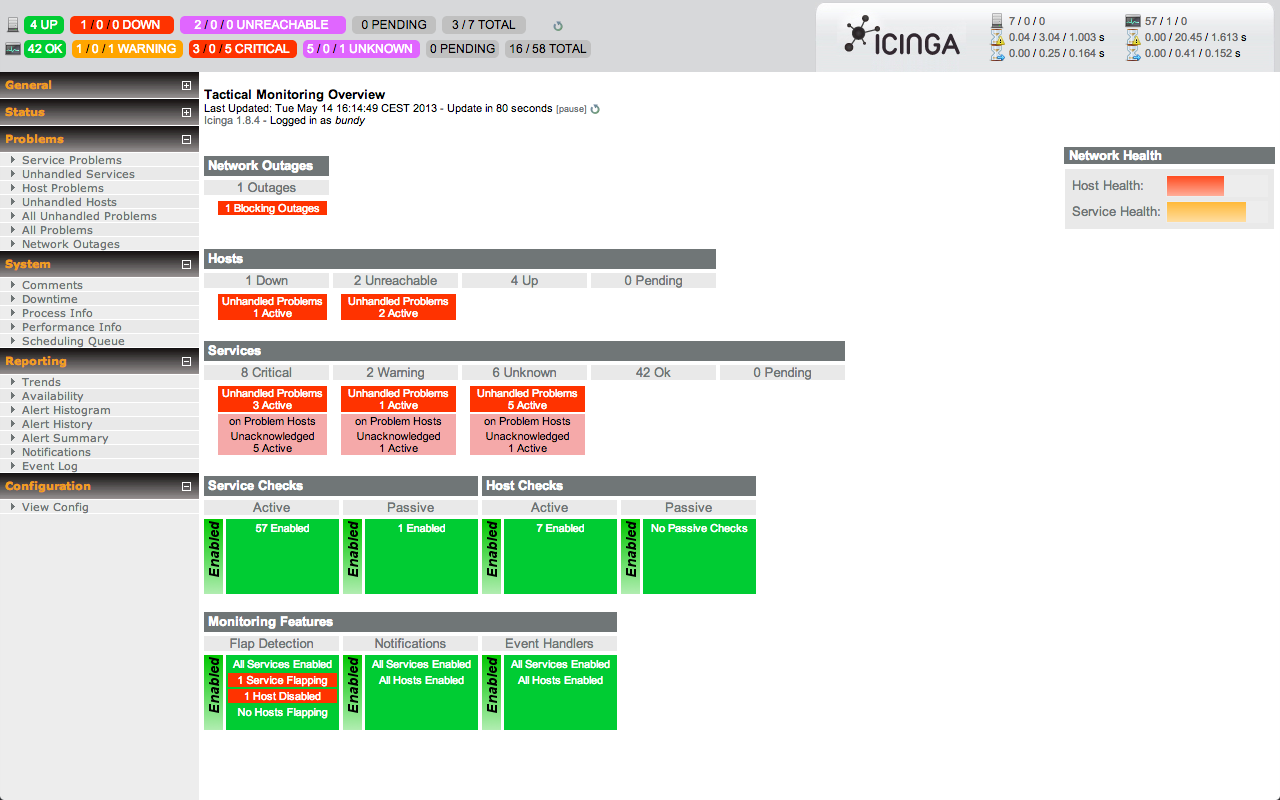
\includegraphics[scale=0.6]{img/icinga_tactical}
    \caption{En visning av "tactical overview" fra webgrensesnittet}
    \label{icingawebgui}
\end{figure}


De som sitter på servicedesk og besvarer henvendelser vil være hovedbrukerene av statusvisningen. Den skal være et hjelpemiddel for å få et overblikk over tjenester og serveres tilstand.

\subsubsection{Design}

For at statusvinduet skulle imøtekomme IKT-avdelingens ønsker, ble det besluttet å gjøre utviklingen i iterasjoner. Ofte vet ikke brukeren hva de vil ha før de ser et utkast og prosessen har begynt. For utviklingen av statusvinduet har designprosessen beskrevet i ISO 9241-210 blitt fulgt. Der er det beskrevet fire aktiviteter som går i syklus til en får et tilfredsstillende resultat:

\begin{itemize}
	\item Understand and specify the context of use
	\item Specify the user and organizational requirements
	\item Produce design solutions
	\item Evaluate designs against requirements.
\end{itemize}

Utviklingsprosessen ble startet med et møte med hele IKT-avdelingen for å presentere gruppens forslag til utkast på designet, som vist i Figur \ref{statusvindu_mockup} mockup. Her kom det frem forslag om å vise temperaturene fra serverrom-sensorene som en terning der det fysiske oppsettet kom frem.

Eksisterende programvare for denne type fremvisning ble funnet etter litt søk, og det ble besluttet å gjenbruke Nagdash cite \cite{nagdash}. Løsningen var et godt utgangspunkt for det visuelle, og er skrevet i språket PHP, noe gruppemedlemmene føler seg komfortable med og IKT-avdelingen har benyttet seg av i tidligere prosjekter. 

Nagdash baserer uthenting av informasjon om host- og serviceobjekter på nagios-api \cite{nagiosapi}, som er en tjeneste som må installeres på Icinga-serveren og setter opp et API over HTTP. Icinga har sitt eget API som det var ønskelig å benytte. Uthenting av informasjon måtte derfor endres til å bruke kall til API-et som Icinga-web tilbyr \cite{icingarestapi}.

Gjennom to iterasjoner kom det frem flere ønsker som ble lagt inn:
\begin{itemize}
	 \item Uthenting av driftsmeldinger via RSS fra portal.hedmark.org
	 \item Endre utseende for “Known Services”
	 \item Sette kolonnene med hosts og servicer ved siden av hverandre 
	 \item Hente ut og grafe antall åpne, lukkede, og mottate saker fra sakssystemet Footprints
	 \item Fjerne irrelevant informasjon som hvilket attempt en gitt service-sjekk er på
\end{itemize}

Det ble også rapportert en bug om at datoen på skjermen ikke endret seg før etter en sideoppfrisking. Koden som oppdaterer datoen var ikke lagt inn i funksjonen som sørger for automatisk oppdatering. Dette viser viktigheten av å ha brukertesting, da en slik bug kan være vanskelig å oppdage.

Etter at all funksjonalitet og design var på plass ble all kode gjennomgått av gruppen i fellesskap for å kvalitetssikre løsningen og sørge for at all ikke-triviell kode var kommentert.

I Figur \ref{statusvindu_mockup} vises en mockup av statusvisningen som vi la fram for IKT-avdelingen ved første møte.

\begin{figure}[H]
    \centering
    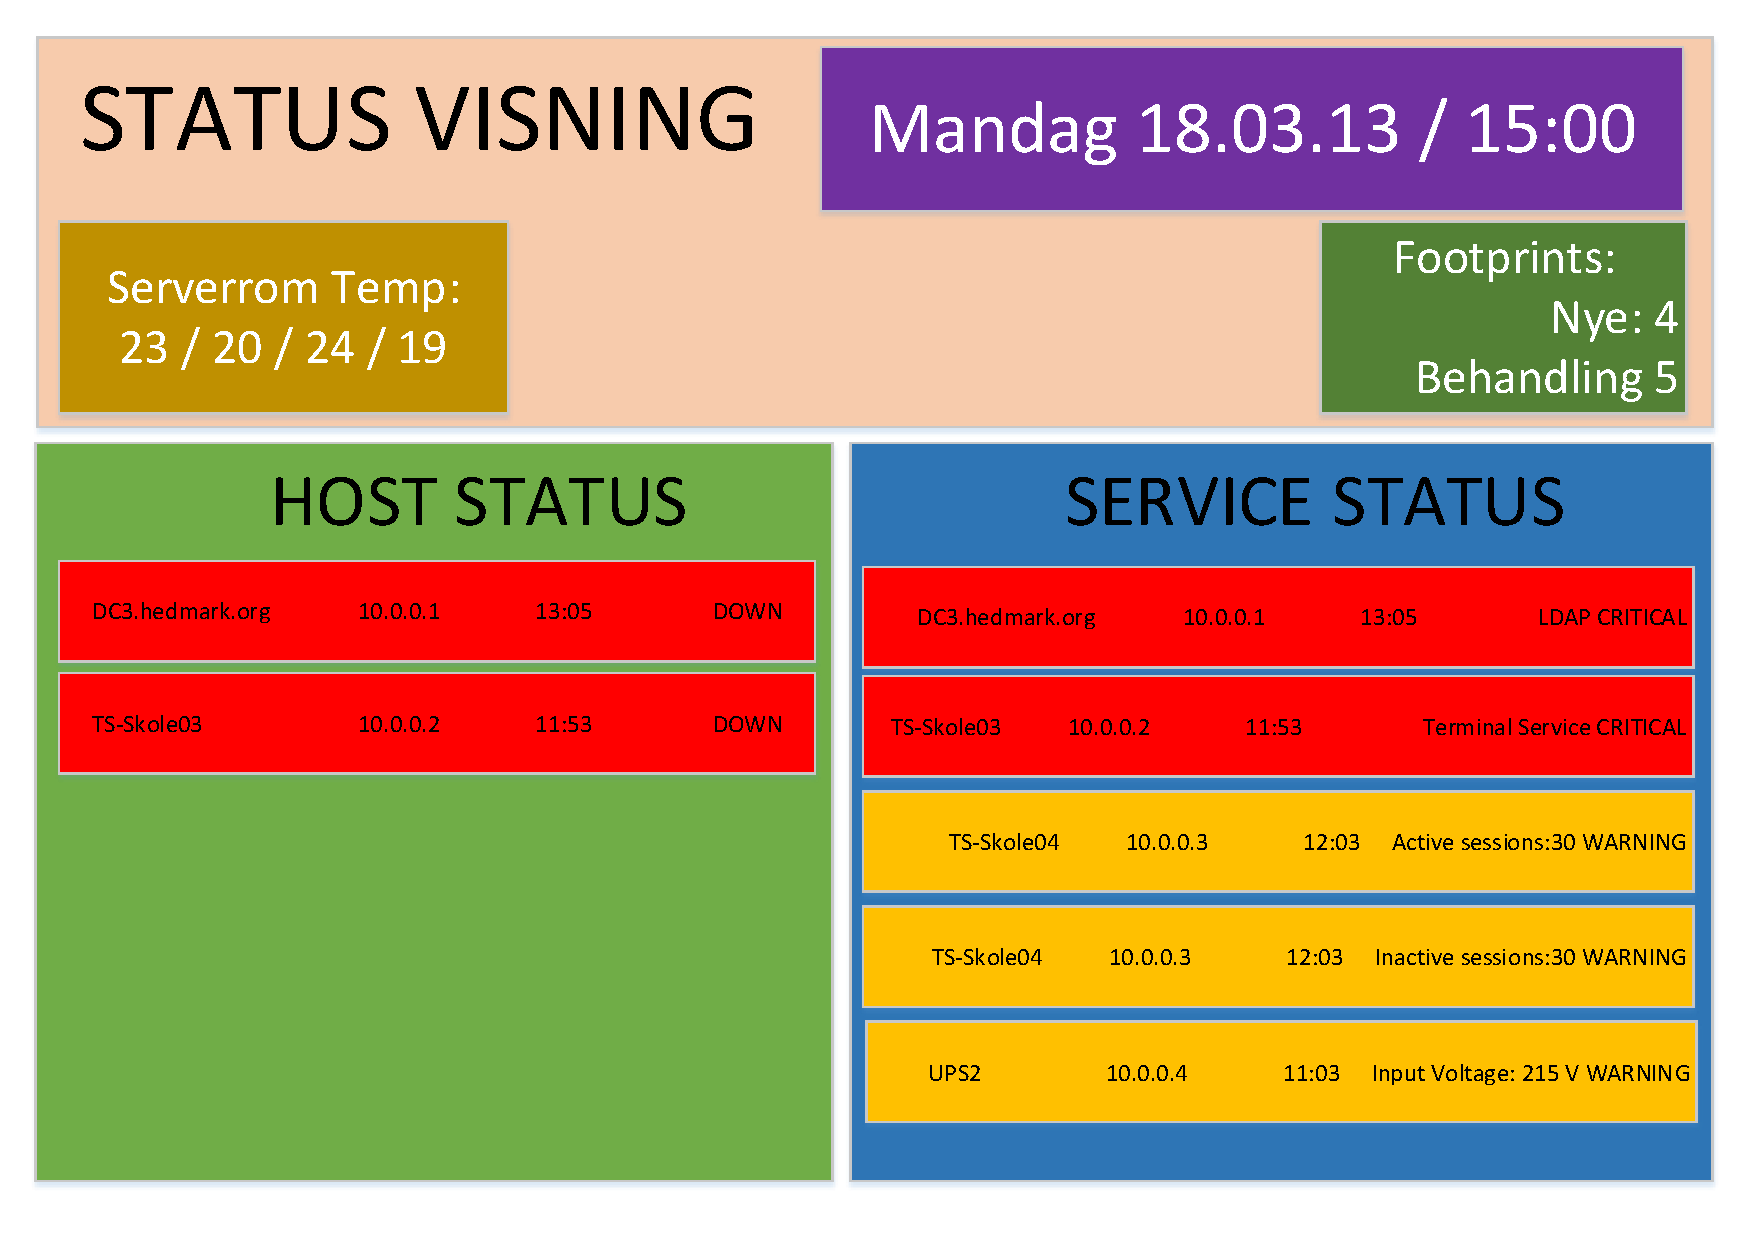
\includegraphics[scale=0.3]{img/statusvindu_mockup}
    \caption{Mockup av statusvindu}
    \label{statusvindu_mockup}
\end{figure}

Figur \ref{statusvindu_mockup} viser hvordan Nagdash ser ut med oversatte API-kall:

\begin{figure}[H]
    \centering
    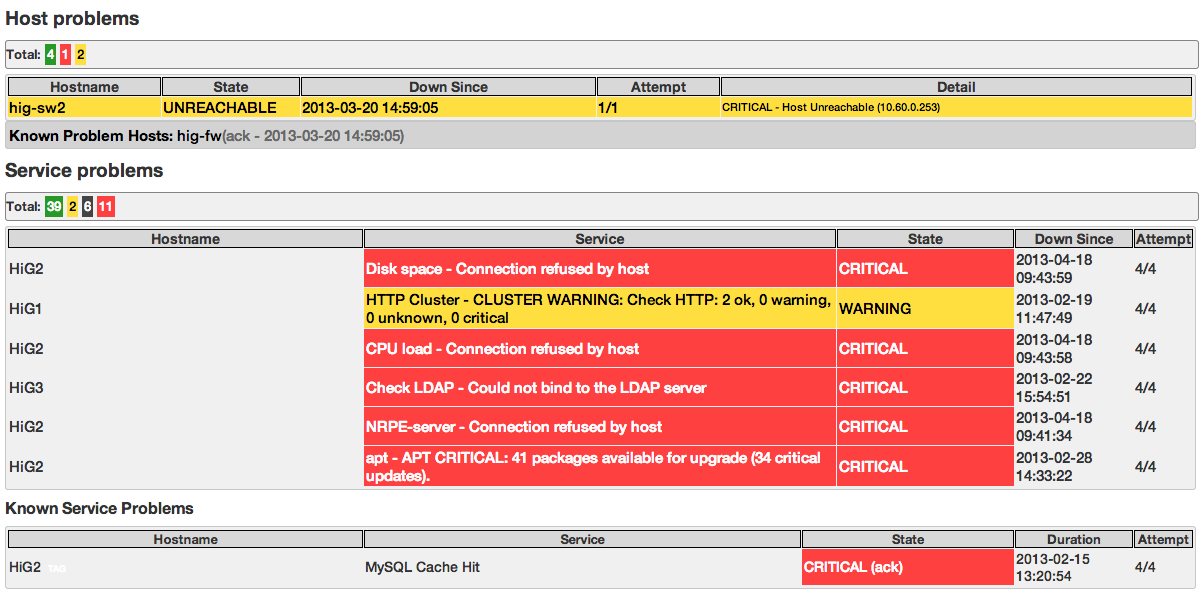
\includegraphics[scale=0.3]{img/statusvindu_oversatte_kall}
    \caption{Statusvindu med oversatte API-kall}
    \label{statusvindu_mockup}
\end{figure}


Figur \ref{statusvindu_first} viser statusvisningen etter første iterasjon, her har følgende funksjonalitet blitt lagt til:
\begin{itemize}
	\item Temperatur fra serverrommet har blitt lagt til
	\item Antall mottate og lukkede saker fra Footprints er lagt til
\end{itemize}

\begin{figure}[H]
    \centering
    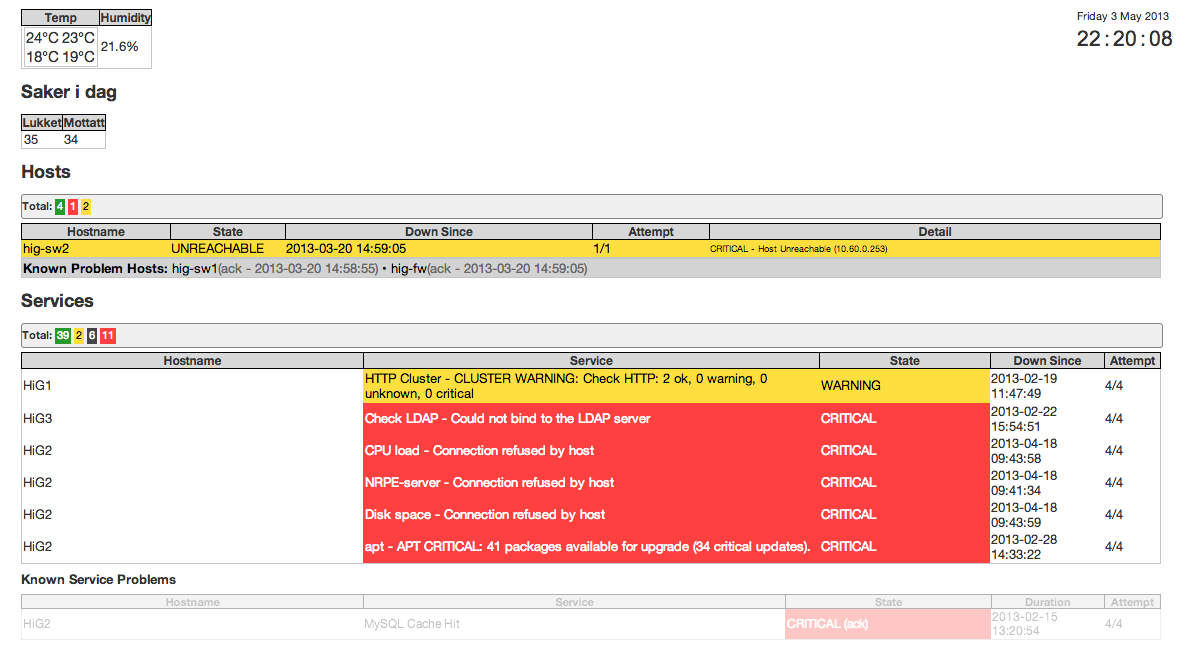
\includegraphics[scale=0.3]{img/statusvindu_first}
    \caption{Statusvindu etter første iterasjon}
    \label{statusvindu_first}
\end{figure}

Figur \ref{statusvindu_final} viser endelig statusvisningen, og her ble følgende funksjonalitet til fra første iterasjon:

\begin{itemize}
	\item Visualisering av retning på luftstrøm
	\item Temperatur fra de sensorene som er konfigurert
	\item Luftfuktighet
	\item Kolonnene for host og services er satt ved siden av hverandre
	\item Driftsmeldinger fra portal.hedmark.org
	\item Grafing av lukkede saker som er mottat i dag, lukkede saker fra alle mottate saker,
	mottate saker i dag og totalt antall åpne saker.
\end{itemize}

\begin{figure}[H]
    \centering
    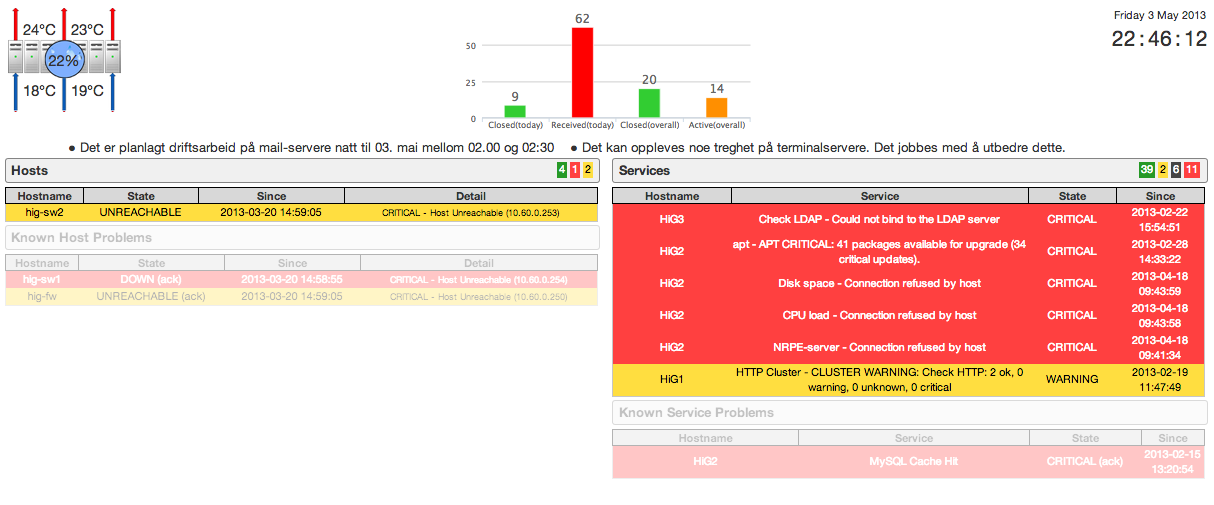
\includegraphics[scale=0.3]{img/statusvindu_final}
    \caption{Sluttresultatet av statusvinduet}
    \label{statusvindu_final}
\end{figure}


\subsubsection{Arkitektur}

Statusvindu definerer strukturen for HTML og inkluderer CSS- og Javascript.

Hver av modulene “footprints.php, netbotz.php og rss.php” retunerer et javascript-objekt med data ut fra ajax-kall fra external.js. Dataene bearbeides og settes inn i riktig “div” i html-en med javascript. Nagdash returnerer rå HTML, da denne inneholder tabeller og annen markup i tillegg til dataene.

I filen external.js hentes data fra de ulike modulene og settes inn i statusvindu dynamisk gjennom Ajax i et bestemt intervall \ref{statusvindu_arkitektur}.

\begin{figure}[H]
    \centering
    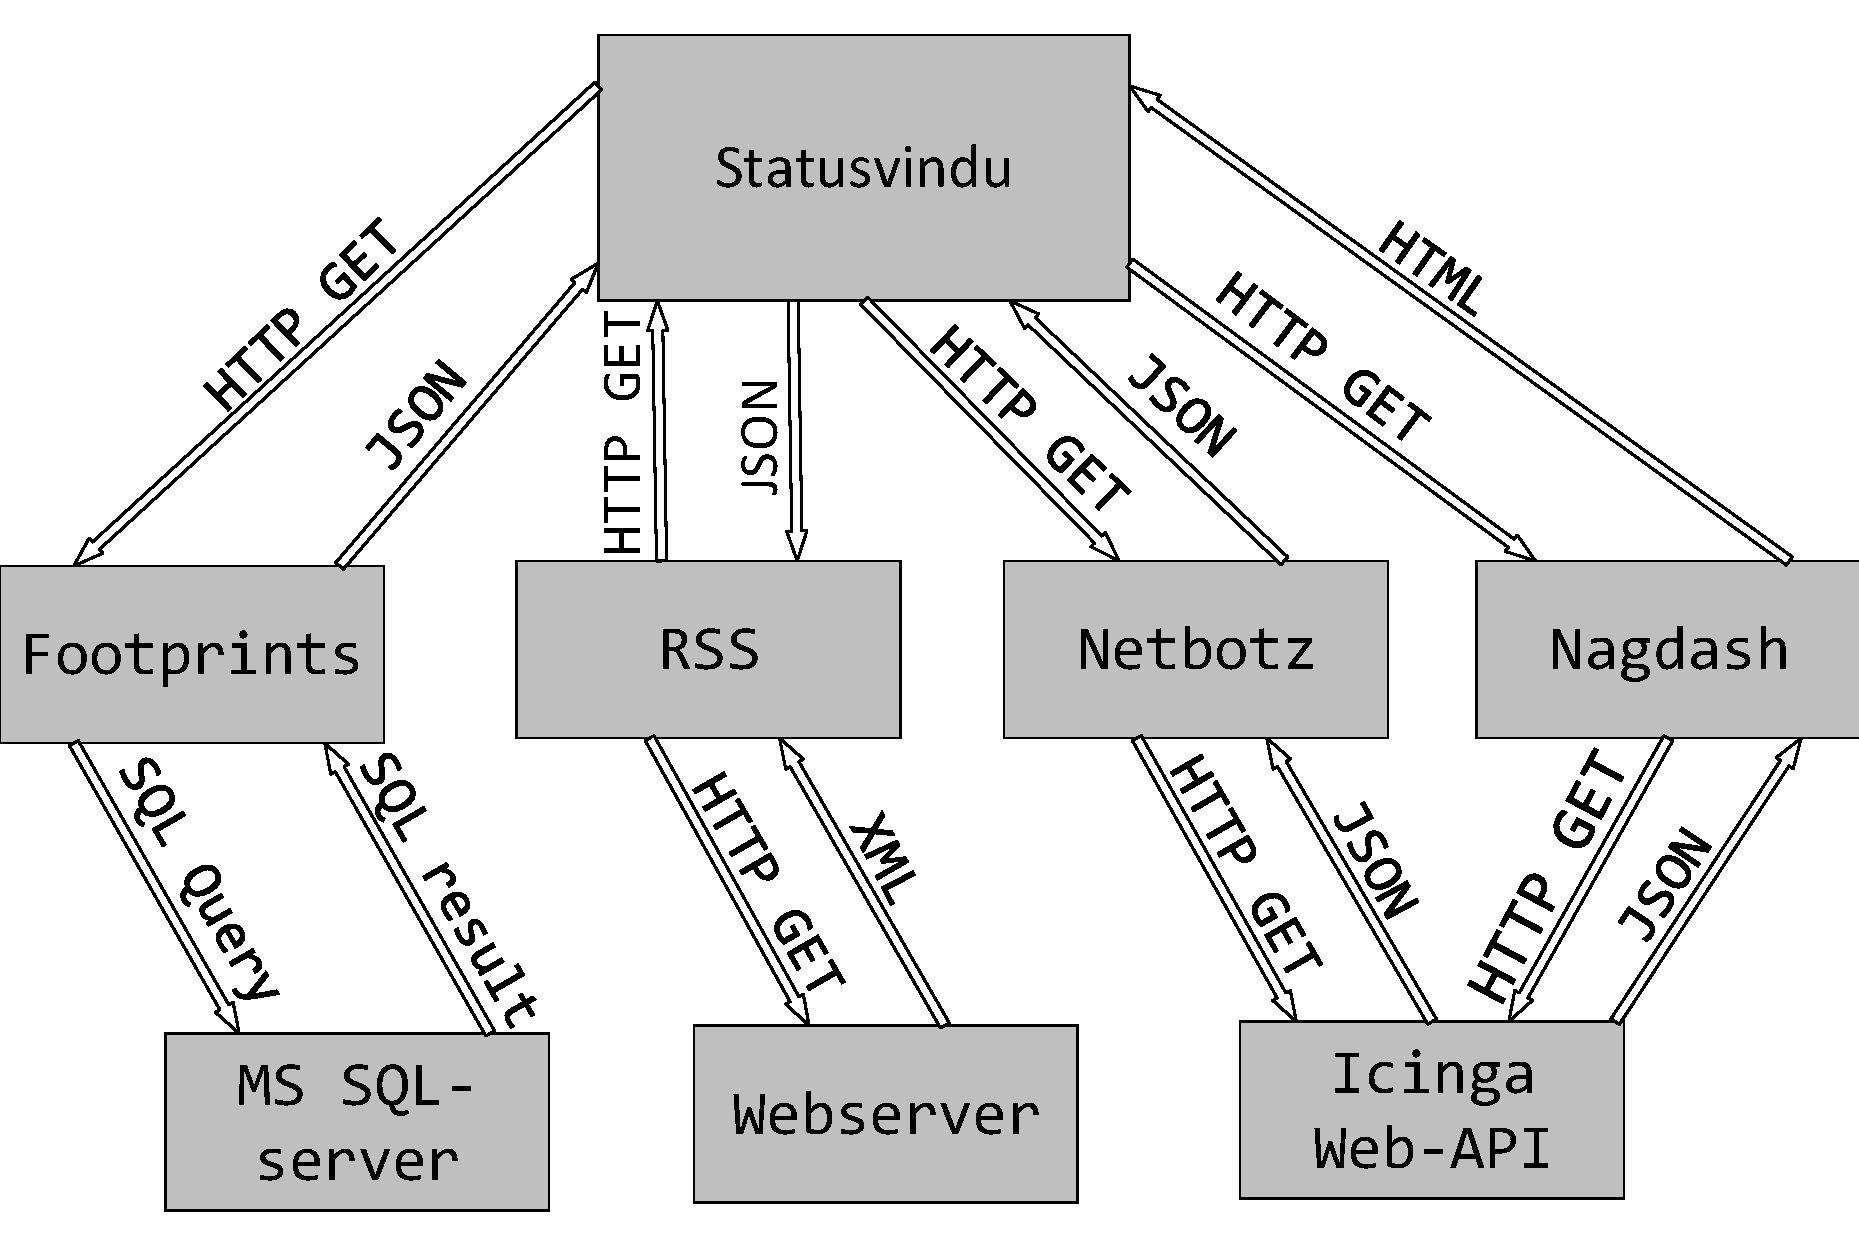
\includegraphics[scale=0.4]{img/statusvindu_arkitektur}
    \caption{Informasjonsflyt mellom modulene involvert i statusvinduet}
    \label{statusvindu_arkitektur}
\end{figure}


\subsubsection{Nagdash}

For å hente ut data fra Icinga benyttes REST-api-et til Icinga-web. I eksempelet under vises en spørring som henter alle host-objekter som har state-en DOWN (HOST\_CURRENT\_STATE|=|1) eller UNREACHABLE (HOST\_CURRENT\_STATE|=|2). Viktige parametere:
\begin{itemize}
	\item <host>: hostnavn eller IP til hosten som kjører Icinga-web
	\item <objekt>: Objekttypen spørringen skal kjøres mot (f.eks host eller service)
	\item filter: Kolonner som skal brukes i sammen med de logiske operatorene AND og/eller OR
	\item columns: kolonner som skal returneres i resultatet
	\item authkey: Nøkkelen brukt for å autentisere til API-et
\end{itemize}

\begin{lstlisting}
http://<host>/icinga-web/web/api/<objekt>/filter[OR(HOST_CURRENT_STATE|=|1;HOST_CURRENT_STATE|=|2)]/columns[HOST_ID|HOST_CURRENT_CHECK_ATTEMPT|...]/authkey=<apikey>/json
\end{lstlisting}

Da får en et javascript objekt ut med de kolonnene en har bedt om.

Vi har totalt 6 spørringer og de ulike gjør følgende:
\begin{enumerate}
	\item  hostQuery henter ut alle hosts som har status DOWN eller UNREACHABLE
	\item  serviceQuery henter ut alle servicer som har en UP host, men en service som er enten WARNING eller CRITICAL
	\item  hostTotalQuery henter ut alle hosts, med en kolonne som forteller hvilken tilstand den er i. Dette blir brukt for å regne ut et antall innen for hver tilstand.
	\item  serviceTotalQuery samme som 3., men henter alle servicer.
	\item  hostPriorityQuery henter ut en og en host basert på objekt id. Informasjonen brukes videre for å sjekke om den har en prioritets variabel satt, som vil føre til at den blir prioritert ved fremvisning.
	\item  servicePriorityQuery samme som 4., men henter her ut for en service
\end{enumerate}

\subsubsection{Footprints}

For uthenting av antallet saker innenfor ulike kategorier i Footprints ble det benyttet SQL-spørringer direkte mot databasen. IKT-avdelingen ønsket å få en graf om følgende antall om saker:
\begin{itemize}
	\item Mottat i dag
	\item Både lukket og mottat i dag
	\item Lukket av alle mottate saker
	\item Antall aktive saker
\end{itemize}

I footprints.php vil returnert data fra alle de 4 spørringene bli slått sammen til et array som videre returneres som et JSON-objekt til external.js via AJAX. 

For å grafe returnert resultat i external.js ble jQuery biblioteket Highcarts benyttet. Det ble først testet et annet bibliotek for grafing: jqBarGraph, men dette hadde manglende konfigurasjonsmuligheter.  

I utdraget nedenfor vises koden for å definere hver søyle i diagrammet (“categories”), og sette de ulike dataverdiene med stats.<variabel>:
\begin{lstlisting}
xAxis: {
   categories: ['Closed(today)', 'Received(today)', 'Closed(overall)', 'Active(overall)']

series: [{
         name: 'Amount',
         data: [{ y: stats.Closed,
                  color: '#32CD32'},
                { y: stats.Received,
             color: '#FF0000'},
                { y: stats.ClosedAll,
             color: '#32CD32'},
                { y: stats.Open,
             color: '#FF8F00'}
               ]
         }]
\end{lstlisting}

Visning søylene uten tall ga bare visualisering av forholdet mellom de ulike kategoriene, så det ble lag til konfigurasjon for å vise selve antallet over hver søyle, slik: 

\begin{lstlisting}
dataLabels: {
               enabled: true,
               style: {
                  fontSize: "16px",
                  lineHeight: "auto"
               }
\end{lstlisting}

Standard font-størrelse var for liten, så denne ble justert opp. I Internet Explorer 9.0 ble da tallet flyttet for høyt over søylen i forhold til standard høyde. En løsning på dette ble funnet via siden for rapportering av feil til Highcharts \cite{iebug}. 

Endring:

\begin{lstlisting}
lineHeight: "auto"
\end{lstlisting}

Figur \ref{IE_bug} viser høydeforskjellen, høyre er før endring og venstre etter:

\begin{figure}[H]
\centering
\begin{subfigure}
  \centering
  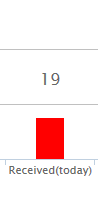
\includegraphics[scale=0.7]{img/IE_footprints_bug}
\end{subfigure}
\begin{subfigure}
  \centering
  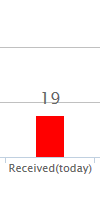
\includegraphics[scale=0.7]{img/IE_footprints_fix}
\end{subfigure}
\caption{Høydeforskjell for antall over hvert søylediagram i Internet Explorer 9.0}
\label{IE_bug}
\end{figure}



\subsubsection{Netbotz}

Det var ønskelig at det skulle være enkelt å legge til nye sensorer for temperatur og luftfuktighet. Alle sensorene oppdages automatisk av pluginen som utførerer sjekkene for Icinga. Via API-et til Icinga-web hentes siste verdi for denne sjekken ut. Samtidig får en ut hvilken ID hver av sensorene har fått. I Javascript mappes hver sensor til riktig rad.

Utdrag fra external.js
\begin{lstlisting}
 var front_layout = [2, 1]; // The netbotz sensor IDs for the front row
  var back_layout = [5, 4];  // and the back
  var columns = Math.max(front_layout.length, back_layout.length); // Largest row is used 
...
  var room = new Image(); // Set up background image for the div
  room.onload = function() {
      $('#serverroom_climate').css('width', this.width);
      $('#serverroom_climate').css('height', this.height);
      $('#serverroom_climate').css('background-image', 'url(' + this.src + ')');
   };

   // Set the background image to be one with the right number of columns
   room.src = "image.php?sensor_cols=" + columns;
\end{lstlisting}

Grafikken for servermiljø tilpasses automatisk etter den raden med flest antall sensorer, ved å lime sammen riktig antall bilder dynamisk gjennom GD i PHP. (se image.php i vedlegg x.x).

\subsubsection{RSS}

RSS-feeden hentes inn fra IKT-avdelingens egen driftsfeed, der meldinger til alle brukere legges ut. Dersom det ikke er noen meldinger vil det ikke vises noe. Hvis lengden på feeden overstiger det som får plass på én linje vil den begynne å scrolle bortover. Dette gjøres med jQuery-pluginen \cite{jqmarquee}.

\subsubsection{Prioritering}

Standard visning av et varsel er å vise den som kom inn sist øverst. Ved tilfeller der det er flere varsler, var det ønskelig å kunne gi en prioritering for å få de viktigste varslene til å komme øverst i listen. For å prioritere host-objekter som er DOWN eller UNREACHABLE og service-objekter som har WARNING eller CRITICAL i statusvisningen, ble to løsninger vurdert. 

Den ene metoden var å bruke et severity-tall som Icinga kalkulerer basert på hvor mange child-hosts og child-servicer som hører til et gitt host-objekt som er nede. Dette vises som “network outages” i Icinga Classic Web der hver host får et “severity”-tall. Det eksisterte ikke noen dokumentasjon om dette kunne hentes ut via API-et eller hvordan “severity” kalkuleres. 

Utrekningen skjer i outages.cgi, som ble funnet etter å lese gjennom HTML-koden og lese kildekoden for outages.c \cite{dnsmichi} : 
Child-servicer blir delt på et forhåndsdefinert tall (service\_severity\_divisor) som brukes for å angi hvor kritisk det er i forhold til child-hosts.

\begin{lstlisting}
temp_hostoutage->severity = (temp_hostoutage->affected_child_hosts + (temp_hostoutage->affected_child_services / service_severity_divisor));
\end{lstlisting}

Det kalkulerte tallet baseres på at hosten som er nede er parent til en eller flere andre hosts. Dette er ikke alltid tilfellet, og metoden vil da ignorere alle host-objekter som ikke er en parent. En annen svakhet er at antall services vil bli kalkulert mot en statisk variabel, som ikke nødvendigvis gjengir viktigheten.

Eksempel:
\begin{equation}
service\_severity\_divisor = 4 
\end{equation}
En host med en child-host som kjører to servicer som er viktige
\begin{equation}
Severity = 1 + (2/4) = 1.5
\end{equation}

En host med to child-hosts som kjører to servicer hver, men er ikke like viktige som nr. 1
\begin{equation}
Severity = 1 + (4/4) = 2
\end{equation}

Metoden er ikke anvendelig for prioriteringen, da det skal kunne settes på hvilken som helst service eller host, og den gjengir ikke viktigheten godt nok.     

Den andre metoden gruppen kom frem til var å sette en egendefinert variabel “\_PRIORITY” på host- og service-objekter, og å hente ut variabelen via API-et til Icinga-web.

Metoden med egendefinert variabel ble valgt, fordi denne kan anvendes på alle servicer og hosts, og gir et bedre prioriteringsgrunnlag enn severity som vurderer antall childs, noe ikke alle hosts nødvendigvis har. En kan heller ikke prioritere en service med metode 1.

Implementasjonen av metode to blir gjort ved å spørre API-et for hver host eller service som er hentet ut fra det første kallet (ref x.x). Har hosten eller servicen variabelen \_PRIORITY definert, vil denne lagres, ellers blir det satt 0 som prioritetstall.

Selve sorteringen av hosts og servicer blir gjort av PHP-funksjonen usort() med to egenskrevne sammenligningsfunksjoner. \cite{usort}. Grunnen til dette er at arrayet er flerdimensjonalt, så det må sorteres på verdien til en spesifikk nøkkel. Det skal også sorteres innenfor tilstandene DOWN og UNREACHABLE, og CRITICAL og WARNING. DOWN skal gå foran UNREACHABLE for host-objekter, og CRITICAL foran WARNING for service-objekter, deretter sorteres det etter prioriteringsvariabelen.

\chapter{Sikkerhet}\label{chap:sikkerhet}
Informasjon som brukes av overvåkningsserveren til å avgjøre tilstanden til en enhet eller tjeneste kommer fra eksterne kilder. Plugin-er vil ha eksekveringstillatelse på eksterne enheter, og SNMP trap-meldinger sender informasjon via en port på overvåkningsserveren. Fokus for prosjektet har vært implementasjon, men det er tatt noen sikkerhetsvurderinger underveis. Ulike sikkerhetsrisikoer og hvilke implikasjoner dette har for imlementasjonen vil bli gått gjennom i dette kapittelet.
\clearpage

\section{Plugin-er}
Flere plugin-er har blitt installert i etterkant av Icinga, og dette utgjør en viss sikkerhetsrisiko. Flere plugin-er har et omfang på 1000 - 5000 linjer og det er en tidkrevende prosess å kvalitetsikre alle. De sjekkene som eksekveres på andre enheter, og ikke på selve Icinga-serveren, er plugin-er som kommer med nagios-plugins og NSclient++. Disse blir brukt av et stort antall organisasjoner og andre. Gruppen har også fulgt med på fora og i kommentarfelt for de ulike plugin-ene for å kunne være trygge på de plugin-ene som kjører på hver enkelt host. 

De plugin-ene som sjekker en tjeneste eller henter ut informasjon som check\_dns, og check\_dhcp har i utgangspunktet ingen mulighet for å kjøre direkte på en host. Disse kan utføre ondsinnede handlinger på selve Icinga-serveren. Alle plugin-er som er tatt i bruk kommer enten i fra monitor-exchange.org, op5, opsview, eller nagios-exchange.

\section{Nettverk}
Icinga-serveren står i et adskilt VLAN. Ved hjelp av pakkefiltrering sperres innkommende trafikk fra andre nettverk. Icinga-serveren må kontakte andre servere den skal overvåke og kommunikasjon som er initiert av Icinga tillates i brannmuren. 

Utstyr som skal sende SNMP-traps til Icinga må få åpnet tilgang i brannmurene som krysses på ruten. Kommunikasjonen fra Icinga-serveren og ut til andre servere rutes gjennom VLAN, som ikke inneholder kommunikasjon fra periferiutstyr. For at denne kommunikasjonen skal kunne sniffes må disse nettverkene være kompromittert.

\subsubsection{SNMP}
I implementasjonen er det benyttet SNMP v2c for alt utstyr som støtter det. I noen få tilfeller har bare v1 vært støttet. Både v1 og v2c benytter autentisering basert på en klar tekststring kalt ``community string''. Det er heller ingen integritetssjekk som verifiserer at kommandoen som ble sendt er den samme som kom fram. Dette er viktigere dersom en sender ``write-kommandoer'', men i dette prosjektet benyttes bare ``read'' for å hente ut informasjon.

I SNMP v3 er det mange muligheter for økt sikkerhet:
\begin{itemize*}
	\item Konfidensialitet. Kryptering. DES
	\item Integritet. Hashing med MD5 eller SHA
	\item Autentisering. Det kan settes rettigheter for spesifikke OID-er for definerte brukere
\end{itemize*}
Overgang til SNMPv3 vil medføre en konfigurasjonsendring på alle enheter som skal overvåkes. En vil også måtte bytte ut eller endre en del plugin-er da disse benytter SNMPv2 eller v1.
\subsubsection{NRPE}
For kryptering og gjenkjenning av hosts har NRPE implementert OpenSSL med en anonymous Diffie-Hellmann. Plugin-en bruker h-filen dh.h til å generere base-nummer og prim-nummer for diffie-hellmann nøkkelutveksling. Disse blir satt statisk ved kompilering av kildekoden, noe som vil si at det er likt for alle debian-pakkene. Etter autentisering av host og Icinga-serveren brukes AES 256 bit for kryptering av trafikk\cite{nrpessl}.

NRPE blir som nevnt tidligere i \ref{sec:nrpe} brukt for å eksekvere kommandoer på eksterne maskiner, og kan være en angrepsvektor både fra overvåkningsserveren og via andre enheter til de den er installert på. Den eksterne maksinen som NRPE blir installert på vil åpne opp for sikkerhetsrisikoer, men det er fortsatt tilpasninger som kan gjøres for å unngå tilgang for uvedkommende og utførelse av ondsinnede handlinger. I konfigurasjonen må en definere hvilke hosts som skal kunne kommunisere med serveren, en må da vite hvilke IP-er som er definert i denne listen. Her vil overvåkningsserveren  i de fleste tilfeller være en definert IP, og da kan det spoofes om denne er kjent for en angriper. En kan også via konfigurasjonen endre porten eksterne enheter skal lytte på. Standardisert port kan finnes i dokumentasjonen så denne bør endres for å skjule tjenestenavn ved portscanning.

Videre utvidelse av implementasjonen av NRPE vil være å ta i bruk forhåndssignerte sertifikater 
som NSClient++ støtter, det vil da føre til en sikrere nøkkelutveksling enn dagens som bare baseres på et prim- og basenummer som er definert ved kompilering.

I konfigurasjonen for NRPE på Linux-servere brukes direktivet ``dont\_blame\_nrpe=1''. Uten dette vil det ikke tillates å sende argumenter til sjekker som skal kjøres.
\subsubsection{NSClient++}
For Windows som bruker NSClient++ kan det settes opp passord som i tillegg kreves for kommunikasjon, dette legger enda et lag med sikkerthet.
allow\_nasty\_meta\_chars, gjør at WMI-spørringer kan sendes som parameter til check\_nrpe og ikke blir regnet som skadelige når NSclient++ mottar de. Dette er fordi en del karakterer vanligvis ville blitt escapet.

I konfigurasjonesfilen for NSClient++ defineres serveradressen slik at kun Icinga-serveren har tilgang til å koble til via NRPE. Dersom denne settes opp til å inkludere et subnett eller inneholder feil adresse vil det være mulig for andre enheter enn Icinga-serveren å koble seg til NRPE-agenten.

\section{Brukerkontoer}
En brukerkonto ble opprettet i Active Directory for Icinga. Denne benyttes ved tilkobling mot domenet på flere områder:
\begin{itemize*}
	\item Sjekk av LDAP.
	\item Synkronisering av kontakter.
	\item Tilkobling mot MSSQL database.
	\item Tilkobling til VMware (Read-only i Virtual Center).
\end{itemize*}
Brukeren som brukes for XenServer har rollen Pool Admin, da IKT-avdelingen bruker en versjon som ikke har funksjonen ``Role Base Access Control''. 

\subsection{LDAP}
LDAP benyttes ved synkronisering av kontakter og kan benyttes til innlogging i Icinga Web og Icinga Classic, som beskrevet i \ref{sec:ldapauth}. LDAP over SSL kan benyttes for å kryptere denne kommunikasjonen. Da må et sertifikat installeres på Icinga-serveren.

\subsection{Databaser}
For MSSQL benyttes en bruker opprettet i Active Directory for autentisering. Denne brukeren får minimale rettigheter slik at den kun kan lese administrative tabeller. I MySQL trenger hver server en egen bruker, denne får også minimale rettigheter, altså kun tilgang til å lese databasen ``INFORMATION\_SCHEMA''. For hver Oracle instanse kreves en egen bruker som har tilgang til se logger, statistikk og status for instansenen, her lages en bruker med SELECT for disse tabellene.

I tillegg til at brukeropprettingsscriptene er fra et firma som jobber med open source overvåkning av database-servere har alle brukeropprettingene blitt gjennomgått med databaseansvarlige ved IKT-avdelingen. 




\chapter{Dokumentasjon}
Gjennom prosjektet har det blitt skrevet egen kode, installert ulike pakker, og satt opp konfigurasjon spesifikt for denne overvåkningsløsningen. Dette kapittelet vil gå igjennom implementering av ulike komponenter som gruppen anser som nødvendig å forklare grundigere.

I Figur \ref{hostfigur} ser vi hvilken generics de forskjellige hostene skal ha.

\begin{figure}[H]
    \centering
    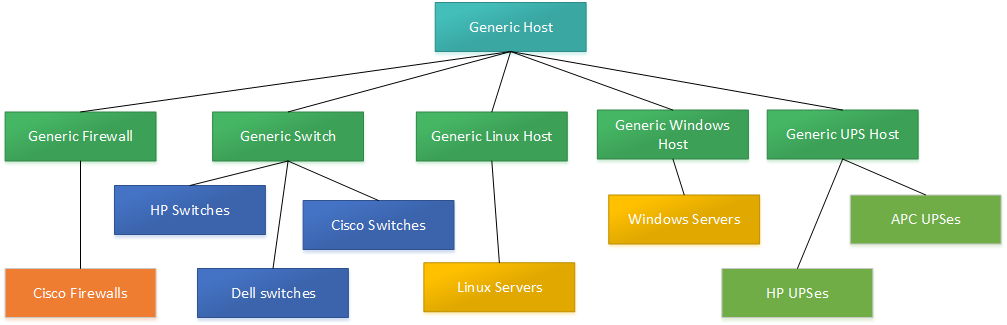
\includegraphics[scale=0.5]{img/host}
    \caption{Oversikt over host generic plassering}
    \label{hostfigur}
\end{figure}

I Figur \ref{hostgroupfigur} ser vi hvilke hostgroups de forskjellige hostene skal være medlem av.

\begin{figure}[H]
    \centering
    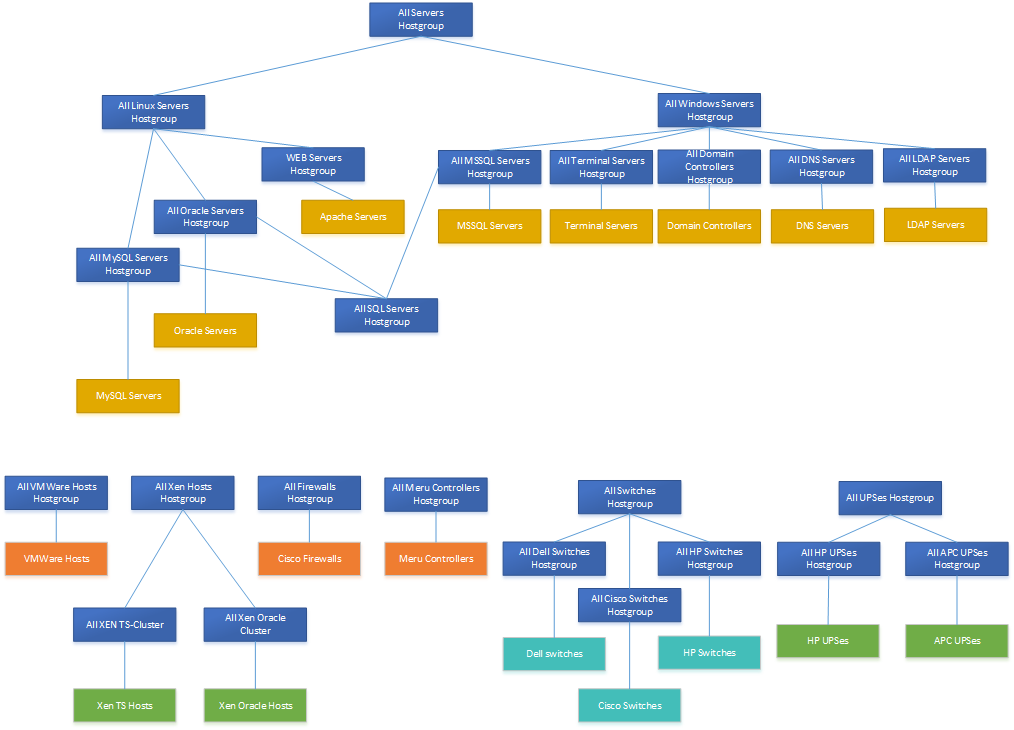
\includegraphics[scale=0.5]{img/hostgroups}
    \caption{Oversikt over hosts hostgroupplassering}
    \label{hostgroupfigur}
\end{figure}

\section{Legge til mange host-objekter}
I utrullingsfaser vil det være naturlig å legge til mange hosts på den gang. Ved å bruke "gen.bash"-scriptet spares tid samtidig som scriptet sørger for å generere hostfilene syntaktisk korrekte.

Scriptet genererer host-objekter med atributtene  ``hostname'', ``address'', ``hostgroup'' og ``generic''. Host-objekter uten hostgroup eller generic supplert, vil få standardverdier definert, mens hostname og address er obligatrisk, og det gis en feilmelding om disse er utelatt.

Eksempelet under viser hvordan scriptet kjøres og at linjenummer skrives ut dersom informasjon som er obligatorsk mangler.
\begin{lstlisting}
monkey@hig1:~/script$ vim servers.csv
monkey@hig1:~/script$ ./gen.bash servers.csv

	Generating hosts from servers.csv into working directory

	Hostname and Address are mandatory.
	Missing for host on line nr: 4
	Missing for host on line nr: 6
	Missing for host on line nr: 7
	Missing for host on line nr: 8

	Done
	Successfully created 4 hosts
	4 hosts where not created because of errors.
monkey@hig1:~/script$ ls
gen.bash  servers.csv  test1.cfg  test2.cfg  test3.cfg  test4.cfg
monkey@hig1:~/script$
\end{lstlisting}

Koden under viser hvordan servers.csv er bygget opp. Inneholder også feil for å vise hva som skjer dersom informasjonen ikke er korrekt.
\begin{lstlisting}
10.0.0.1,test1,windows;,generic1
10.0.0.1,test2,,jekrjekr
10.0.0.1,test3
,,,
10.0.0.1,test4
1,
,
,
\end{lstlisting}

Kildekoden til scriptet ligger i Vedlegg \ref{gen.bash}.

\section{Forventet nedtid}
Tilfeller kan forekomme hvor en server må tas ut av drift på grunn av vedlikehold. I Icinga er det ikke nødvendig å fjerne denne fra konfigurasjonen, for å unngå at varslingsmelding blir sendt ut. I både Icinga Web og Icinga Classic har man mulighet til å bruke en funksjon som kalles ''Schedule Downtime''. Her blir nedetidens start og slutt definert.

I den nedetidsperioden vil Icinga nekte varslingsmelding i å bli sendt ut. Når nedetidsperioden er ferdig, eller denne blir utført før avtalt tid, vil kontaktene som skal bli varslet få en melding om at nedetid er over, og Icinga vil ikke lengre holde igjen varlser.

\section{Stoppe varsling}
acknowledge, stopper gjenvarsling??
\section{Autentisering mot Active Directory} 
LDAP-autentisering brukes for å styre hvem som skal ha tilgang til web-grensesnittene, ved hjelp av grupper og brukere i Active Directory. Dette er støttet direkte i Icinga Web, men må konfigureres på andre måter for Icinga Classic. Det kan opprettes en sikkerhetsgruppe i AD som inkluderer medlemmene som skal få tilgang. Alle som er med i denne gruppen vil få tilgang til Icinga Web, der det også kan defineres hvilken informasjon hver bruker skal se. 

Selve LDAP-binden gjøres via PHP-modulen “php-ldap”. Når en bruker logger inn sjekkes først AD, dersom brukeren ikke finnes der, vil Icinga-web prøve sin egen database over brukere. Hvis brukeren finnes her og passordet er riktig vil brukeren bli logget inn. Når brukeren har logget inn for første gang via AD, vil brukeren bli lagret i Icinga Web-databasen. Om brukeren endrer passord i Icinga Web vil uansett AD først bli spurt før Icinga Web spør om passordet er riktig i sin egen database

Icinga classic autentiserer mot AD gjennom modulene ldap og authnz\_ldap.

/etc/apache2/conf.d/
\begin{lstlisting}
        AuthName "Authentication"
        AuthType Basic
        AuthBasicProvider ldap
        AuthLDAPURL
"ldap://10.60.0.22:3268/dc=monkey,dc=local?samAccountName?sub?(objectClass=person)"
        AuthLDAPBindDN "flash@monkey.local"
        AuthLDAPBindPassword "Bachel0r"
        require ldap-group CN=icinga-login, OU=icinga, DC=monkey, DC=local
\end{lstlisting}

/usr/share/icinga-web/app/modules/AppKit/config/auth.xml
\begin{lstlisting}
  <ae:parameter name="ldap_allow_anonymous">false</ae:parameter>
            <ae:parameter name="ldap_dsn">ldap://10.60.0.22</ae:parameter>
            <ae:parameter name="ldap_start_tls">false</ae:parameter>
            <ae:parameter name="ldap_basedn">DC=monkey,DC=local</ae:parameter>
            <ae:parameter name="ldap_binddn">icingawebauth@monkey.local</ae:parameter>
            <ae:parameter name="ldap_bindpw"><![CDATA[Password]]></ae:parameter>
            <ae:parameter name="ldap_userattr">sAMAccountName</ae:parameter>
            <ae:parameter name="ldap_filter_user"><![CDATA[(&(sAMAccountName=__USERNAME__)(memberOf=CN=icinga-login,OU=icinga,DC=monkey,DC=local))]]></ae:parameter>
        </ae:parameter>
\end{lstlisting}

\section{Kontakter og kontaktgrupper}

For å opprette en ny kontakt i Icinga meldes brukeren inn i gruppen icinga\_kontakter (se synkronisering). Den vil trenge å ha e-postadresse og telefonnummer satt.

Kontaktgrupper hentes fra OU-en icinga\_grupper der alle grupper hentes ut og opprettes i Icinga. For at en gruppe skal varsles må dette legges til på en service. For å slippe å sette opp kontakter for hver service kan en velge å sende med argumentet “gen\_service” for å generere en template som kan benyttes på tjenester som sorterer under hver av kontaktgruppene som blir opprettet.

Eksempel på generisk service som blir opprettet:
\begin{lstlisting}
define service {
    name network_services
    register 0
    use generic-service     
    notification_interval   30
    notification_period     24x7
    notification_options    w,c,r
    contact_groups          network_contact_group
}
\end{lstlisting}

Denne brukes på en Cisco firewall: 
\begin{lstlisting}
define service {
        service_description Cisco Firewall CPU Load
        use network_services
        name cisco-firewall-cpu-load
        hostgroup_name all_firewalls
        check_command check_network_component!cpu-load
}
\end{lstlisting}

Tabell med sjekker og tilhørende parametere:
\begin{table}
\begin{center}
\begin{tabular}{| l | l | l | l |}
 \hline
        \textbf{Utstyr} & \textbf{Service navn} & \textbf{Warning} & \textbf{Critical}
	\\ \hline
	APC UPS 		& UPS Capacity			& 90:	& 80: \\ \hline
	APC UPS			& Internal Temp			& 30	& 32 \\ \hline
	APC UPS			& Load				& 50	& 60 \\ \hline
	APC UPS			& Voltage In			& 225:239 & 220:245 \\ \hline
	APC UPS			& Voltage Out			& 225:239 & 220:245 \\ \hline 
	HP UPS			& Battery Time Remaining 	& 3000: & 2700: \\ \hline
	HP UPS			& Battery capacity		& 90: 	& 80: \\ \hline
	HP UPS			& Battery current		& 	& \\ \hline
	HP UPS			& Voltage In			& 225:239 & 220:245 \\ \hline 
	HP UPS			& Voltage Out			& 225:239 & 220:245 \\ \hline
	Windows Server		& Check DNS			& 0.1	& 0.2 \\ \hline
	Windows Server		& Check LDAP			& 0.05	& 0.1 \\ \hline 
	Windows Server		& All Disks			& 94\%	& 96\% \\ \hline
	Windows Server		& Disk Space			& 90\%	& 95\% \\ \hline
	Windows Server		& CPU Load			& 90	& 95 \\ \hline
	Windows Server		& Memory Usage			& 94\%	& 98\% \\ \hline
	Windows Server		& RDP-Sessions: Active		& 20	& 25 \\ \hline
	Windows Server		& RDP-Sessions: Inactive	& 15	& 20 \\ \hline
	Cisco ASA / PIX		& CPU Load			& 93	& 96 \\ \hline
	Cisco ASA / PIX		& Hardware Health		& N/A	& N/A \\ \hline
	Cisco ASA / PIX		& Memory Usage			& 93	& 96 \\ \hline
	Cisco ASA / PIX		& Failover Status		& N/A	& N/A \\ \hline
	Cisco ASA / PIX		& VPN Sessions			& 80 (\% av lisens) & 90 (\% av lisens) \\ \hline
	Dell Blade Chassis	& Dell Blade Server Health	& N/A	& N/A \\ \hline
	Dell Powerconnect	& Assets			& N/A	& N/A \\ \hline
	Dell Powerconnect	& Uptime			& N/A	& N/A \\ \hline
	Dell Powerconnect	& Fans				& N/A	& N/A \\ \hline
	Dell Powerconnect	& Power supply			& N/A	& N/A \\ \hline
	Dell Powerconnect	& Temperature			& 34	& 36 \\ \hline
	HP Procurve		& Environment Status		& N/A	& N/A \\ \hline
	MySQL			& Cache Hit			& 60: 	& 50: \\ \hline
	MySQL			& Health			& 0.1	& 0.2 \\ \hline
	MySQL			& Slow Queries			& 0.1	& 1 \\ \hline 
	MySQL			& User Connections		& 50	& 80 \\ \hline
	MSSQL			& Cache Hit			& 90:	& 80: \\ \hline
	MSSQL			& Health			& 0.05	& 0.15 \\ \hline
	MSSQL			& Lazy Writes			& 20	& 0 \\ \hline
	MSSQL			& User Connections		& 2000	& 2200 \\ \hline
	Oracle			& Cache Hit			& 93:	& 90: \\ \hline
	Oracle			& Connected Users		& 50	& 80 \\ \hline
	Oracle			& Connection Time		& 0.1	& 0.2 \\ \hline
	Oracle			& Free Tablespace		& 5:	& 2: \\ \hline
\end{tabular}
\label{objekt_varsling}
\end{center}
\end{table}

\section{Backup-rutiner}
I Tabell \ref{backup}, vises viktige filer og mapper for overvåkningsløsningen. Disse bør integreres i en backup av Icinga-serveren.
\begin{table} \label{backup}
\begin{center}
\begin{tabular}{| p{8cm} | p{8cm} |}
 \hline
        \textbf{Filbane} & \textbf{Inneholder}
	\\ \hline
	/etc/icinga/						& Alle konfigurasjonsfiler for Icinga \\ \hline
	/usr/lib/nagios/plugins/				& Alle plugin-er \\ \hline
	/etc/nagios-plugins/config				& Konfigurasjon for default plugins \\ \hline
	/root/Scripts						& Lokale script. \\ \hline
	/etc/snmp 						& Konfigurasjon for snmptt \\ \hline
	/etc/default/snmp 					& Konfigurasjon for at snmpd starter snmptrapd \\ \hline
	/etc/sysconfig/icinga					& Konfigurasjon for environment variabler \\ \hline
	/usr/lib/oracle/11.2/client64/network/
	admin/tnsnames.ora					& Konfigurasjon for oracle-instanser \\ \hline
	/etc/init.d/carbon-cache				& Init script for grafprosessering gjennom graphite \\ \hline
	/etc/init.d/metricinga					& Init script for prosessering av perfdata fra Icinga \\ \hline
	/opt/graphite/						& Konfigurasjon og data for genering av grafer  \\ \hline
\end{tabular}
\end{center}
\end{table}
I tilegg bruker Icinga Classic og Icinga Web hver sine databaser, kalt ''icinga'' og ''icinga\_web''. Graphite bruker også en database, som heter ''graphite''.

\chapter{Avslutning}
\section{Evaluering}
\subsection{Gjennomføring av prosjektet}
Da prosjektarbeidet ble satt i gang ble det tidlig registrert at oppgavebeskrivelsen var noe løs/mangelfull/lite konkret. Det var derfor usikkerhet rundt hvor omfattende overvåkningsløsning oppdragsgiver ønsket seg. Dersom kommunikasjonen mellom gruppen og oppdragsgiver hadde vært grundigere fra starten av, og kravspesifikasjonen hadde vært mer konkret, ville dette ført til mindre tid på oppklaring ved senere tidspunkt. Det ville også gitt et større overblikk over hva som skulle gjøres. På grunn av dette ble overvåkningsløsningen mer omfattende og tidkrevende enn først forutsett av gruppens medlemmer.

Fordi vi ønsket å dekke flest mulig av kategoriene ulikt utstyr og tjenester IKT-avdelingen drifter i produksjon, valgte vi å sitte på fylkeshuset to dager i uken. Det ble derfor brukt mye tid på reising til og fra fylkeshuset.

I forhold til det Gantt skjemaet som ble satt opp i forprosjeketet har vi fulgt de iterasjonene som ble satt opp, med noen unntak. Serverrommiljø ble flyttet til etter varsling da enheten for å overvåke serverrommiljøet kom senere enn forventet. Iterasjonene Serverrommiljø og statusvindu ble utført parallelt, grunnet mindre arbeidsmengde enn forventet i serverrommiljø. Vi satt også opp sjekker for UPS-er i infrastrukturiterasjonen, som i utgangspunktet var planlagt for serverrommiljø. Noen tjenester har tatt lenger tid å implementere enn planlagt og disse har blitt jobbet med samtidig som andre iterasjoner har pågått.

Innenfor hver iterasjon var det satt opp faser med planlegging, implementering og en fase med testing og evaluering. Utover i prosjeket ble ikke dette fulgt. Planlegging og evaluering har skjedd mer individuelt for hver enhet og tjeneste som har blitt lagt til i overvåkningen. For alle iterasjonene har det vært møter med statusoppdatering, som planlagt. 

Det ble også mye nødvendig dobbeltarbeid med å implementere sjekker i labmiljøet først og så i produksjon. For noen tjenester var det ikke mulig å teste i labmiljøet først.

Valget av Icinga har ikke hindret oss i å få til det som var ønsket. Arkitekturen Icinga baserer seg på er en enkel kjerne hvor tilleggsfunkjsonlitet må legges til. Dette gir stor frihet, og fleksibiltet fordi en kan utnytte et stort antall tredjeparts pluginer som eksisterer, eller utvikle plugin-er etter behov. 

En overvåkningsløsning basert fri programvare kan ha visse ulemper. Ofte kommer slike løsninger uten support-avtaler, noe en som oftest finner i en properitær løsning. Properitære løsninger markedsføres, og selges, ofte som en komplett pakke der en får produktet sammen med support og support-avtaler. 

tredjeparts kode kan variere og ikke oppfylle alle ønsker, 
arbeidsmengde ved implementasjon av ny funksjonalitet (finne gode plugin og kvalitetssikring), 
variernde dokumentasjon (ikke standardisert) 

\subsection{Organisering av arbeid}
Innad i gruppen har det blitt avholdt daglige møter for å oppdatere resten av gruppen om utført arbeid, og om eventuelle utfordringer som har oppstått. 

Kontakten med veileder har fungert godt med ukentlige møter og hjelpsomme forslag relatert til arbeidet.

Avtalte møter med oppdragsgiver ble til tider ikke avholdt, grunnet at oppdragsgiver ikke alltid var til stede da gruppen var på Fylkeshuset. Fordi oppsatte møtetidspunkter ikke alltid passet, ble gruppen og oppdragsgiver/teknisk kontakt enig om muntlige oppdateringer utenom møtene. Det var dessuten noe vanskelig å få avtalt overføring av funksjoner fra lab til produksjon med de som hadde ansvar for systemet, da disse ikke alltid var tilstede da gruppen var på fylkeshuset. 

Utgangspunktet for utførelsen av prosjektet var at det meste av vårt arbeid skulle skje i et labmiljø. Vi skulle deretter legge fram et forslag til et overvåkningssystem for implementering ved IKT-avdelingen.

Det positive med å ta en større del av implementeringen av overvåkningssystemet er at det er givende å levere en større løsning til oppdragsgiver, og at systemet som er konstruert kan iverksettes slik det nå fremligger.

Ved utvikling av statusvindu endte vi opp med å skrive om nesten all koden i Nagdash. Her gikk det med mye tid, og strukturen på koden ble heller ikke slik gruppen hadde gjort det om det ble skrevet fra bunnen. 

Gjennomgang av ulike plugin-er viste seg å ta mer tid enn forventet. Årsaken var for det meste dårlig dokumentasjon og varierende kodekvalitet. Et tilfelle var check\_xenapi.pl som ble gjennomgått for å sjekke om det var noe gjennomsnittskalkulering på returnert resultat, og om det var mulig å legge dette til. Pluginen bruker 12 ekstra Perl-filer for å sette opp kall til RRD-databasen, og gjennomgang av disse tok for mye av tiden i forhold til gevinsten med å få den implementert. Det var den eneste plugin-en som hadde mer funksjonalitet enn å sjekke statusen for en Xen-host, så det ble priortert å gå gjennom koden for denne. 

Det har i ettertid lært oss at det ikke alltid vil være besparende å gjenbruke kode. Noen ganger kan det faktisk lønne seg å finne opp hjulet på nytt.

-Roller. Gruppeleder ikke vært nødvendig. Komunikasjonsansvarlig bra
\subsubsection{Arbeidsfordeling}
Arbeidet har blitt fordelt slik at den av gruppens medlemmer med størst interesse og/eller kunnskap om et tema har satt seg godt inn i dette. Dette har ført til besparing av tid, da det for det meste har blitt utført tre oppgaver parallelt. Dette var nødvendig for å få tid til å gjennomføre målsetningen som ble satt. Utfordringen med denne fordelingen har vært å oppnå god oversikt over det totale arbeidet for hver av oss. Det tok tid å sette seg inn i problemstillinger når andre medlemmer støtte på vanskelige valg eller problemer, og det var behov for å ta felles avgjørelse.

Jevnlig og god kommunikasjon innad i gruppen har resultert i et godt samarbeid med få problemer. 

\subsubsection{Prosjekt som arbeidsform}
Å utføre et prosjekt for en ekstern organisasjon har vært givende og lærerikt. Det å levere et etterspurt produkt til arbeidsgiver gir et godt innblikk i hvordan arbeidslivet fungerer.

Dog ble mer tid og ressurser brukt på utføringen av bacheloroppgaven enn det som ville blitt med gjenomsnittlige emner med tilsvarende studiepoeng. Dette gjorde at det var utfordrene å følge opp andre fag i tillegg til bacheloroppgaven.

\subsubsection{Subjektiv oppfatning av bacheloroppaven}
Utføringen av bachelorprosjektet har gitt oss mye lærdom om omfattende prosjekter. Dette er relevant når vi nå skal ut i arbeidslivet. Den type erfaring hadde vi ikke tilegnet oss dersom tiden ble brukt i en forelesningsal, og dermed var dette bachelorprosjektet en godt egnet avslutning på utdanningen. 

\section{Videre arbeid}
I denne prosjektoppgaven har hovedfokus vært å bygge opp en overvåkningsløsning som tilfredsstiller kravene i oppgavebeskrivelsen. Det er tatt høyde for tilleggsfunksjonaliteten fra oppgavebeskrivelsen. Hovedsaklig går dette på historisk overvåkning. Det er satt opp grafing av ytelsesdata fra Icinga, men her er det mange muligheter for forbedring og videre arbeid. Dataene kan for eksempel analyseres for å sende varsler til Icinga om trender som indikerer problemer i nær fremtid, for eksempel om bruk av lagringsplass på en filserver.

Parallelt med prosjektarbeidet har IKT-avdelingen gjennomført et prosjekt der en CMDB har blitt implementert. Integrasjon mot denne med konfigurasjon fra objektene i overvåkningen og etterhvert mulighet for å definere avhengigheter som gjenspeiler seg i overvåkningen, kan være aktuelt.

Icinga 2 /cite https://www.icinga.org/about/icinga2/ er under utvikling og er en parallell utviklingsprossess med Icinga 1.x. Planlagt stable release er i slutten av 2013. Icinga 2 er en ny kjerne som skal skrives fra bunnen av og fjerner det som Icinga 1.x har arvet i fra Nagios. Den nye kjernen vil fungere sammen med Icinga 1.x gjennom et kompabilitetslag cite http://en.wikipedia.org/wiki/Compatibility\_layer som oversetter systemkall. Her kan enten migrering til Icinga 2, oppsett av Icinga 2 sammen med eksisterende Icinga 1.x, eller å evaluere Icinga 2 som et nytt verktøy være aktuelt videre arbeid. 

Varsling er implementert slik at statusvisning blir oppdatert og det sendes ut varslingsmeldinger til en eller flere personer over e-post og SMS. Det må altså manuelt opprettes en sak i sakssystemet Fooprints. Her kan det være aktuelt å implementere en automatikk i at ønskede varsler registreres i sakssystemet, med ulike parametre som tjeneste eller host, prioritering, og ansvarlig person.

Asterisk og Trio er to telefonsystemer IKT-avdelingen drifter. Her vil det være relevant å overvåke køer, og annen informasjon. Å integrere dette med Icinga kan være en spennende utfordring å basere en oppgave på.

IKT-avdelingen ved Hedmark fylkeskommune har flere lokale IKT-avdelinger, som i hovedsak løser lokale problemer ved skoler, men som er avhengig av sentrale tjenester som trådløse nettverk og Internett-tilgang. Icinga Web muligheter for tilgangstyring på brukernivå for visning av informasjon. Et mulig prosjekt kan være å gjøre de tilpasningene som må til for å integrere de lokale avdelingene i overvåkningsløsningen. 

\section{Konklusjon}
Det viktigste målet med denne prosjektoppgaven ble oppnådd. En ny overvåkningsløsning ble satt i produksjon med overvåkning av store deler av IKT-avdelingens infrastruktur og servertjenester. Løsningen kjører nå parallelt med den overvåknigsløsningen som fantes fra før, og overvåker mye som den gamle løsningen ikke har mulighet til. Oppdragsgiver planlegger at den eksisterende overvåknigsløsningen skal fases ut over tid, etterhvert som resterende tjenester og enheter integreres i den nye løsningen. 

Etter gruppens mening vil oppgaven kunne tjene som eksempel på de aller fleste tjenester og enheter ved utvidelse av løsningen. I forhold til Servers Alive er vår løsning mer oversiktlig og tilrettelagt for utvidelse, noe som forhåpentligvis fører til mer effektiv drift for IKT-avdelingen.

Gruppen er fornøyd med resultatet som ble overlevert og mener den dekker mer enn de kravene som ble satt. Ved overlevering var ikke alle IKT-avdelings servere og tjenester under overvåkning, men det er lite som skal til for å legge til nye enheter. Dersom det skal legges til nye sjekker vil det som er satt opp tjene som gode eksempler på hva som er mulig, og hvordan en kan legge det opp.

Læringsutbyttet har vært høyt, og vi mener vi har nådd de målene vi satte ved starten av prosjektet. 


% Biblography

\clearpage
\bibliographystyle{ieeetr}
%\bibliographystyle{te}

\addcontentsline{toc}{chapter}{Referanser}
\small{\bibliography{rapport,rapport-books}}
\clearpage

% Appendixes
\pagestyle{plain}
\begin{appendices}
\clearpage
\chapter{Arbeidslogg}\label{app:arbeidslogg}
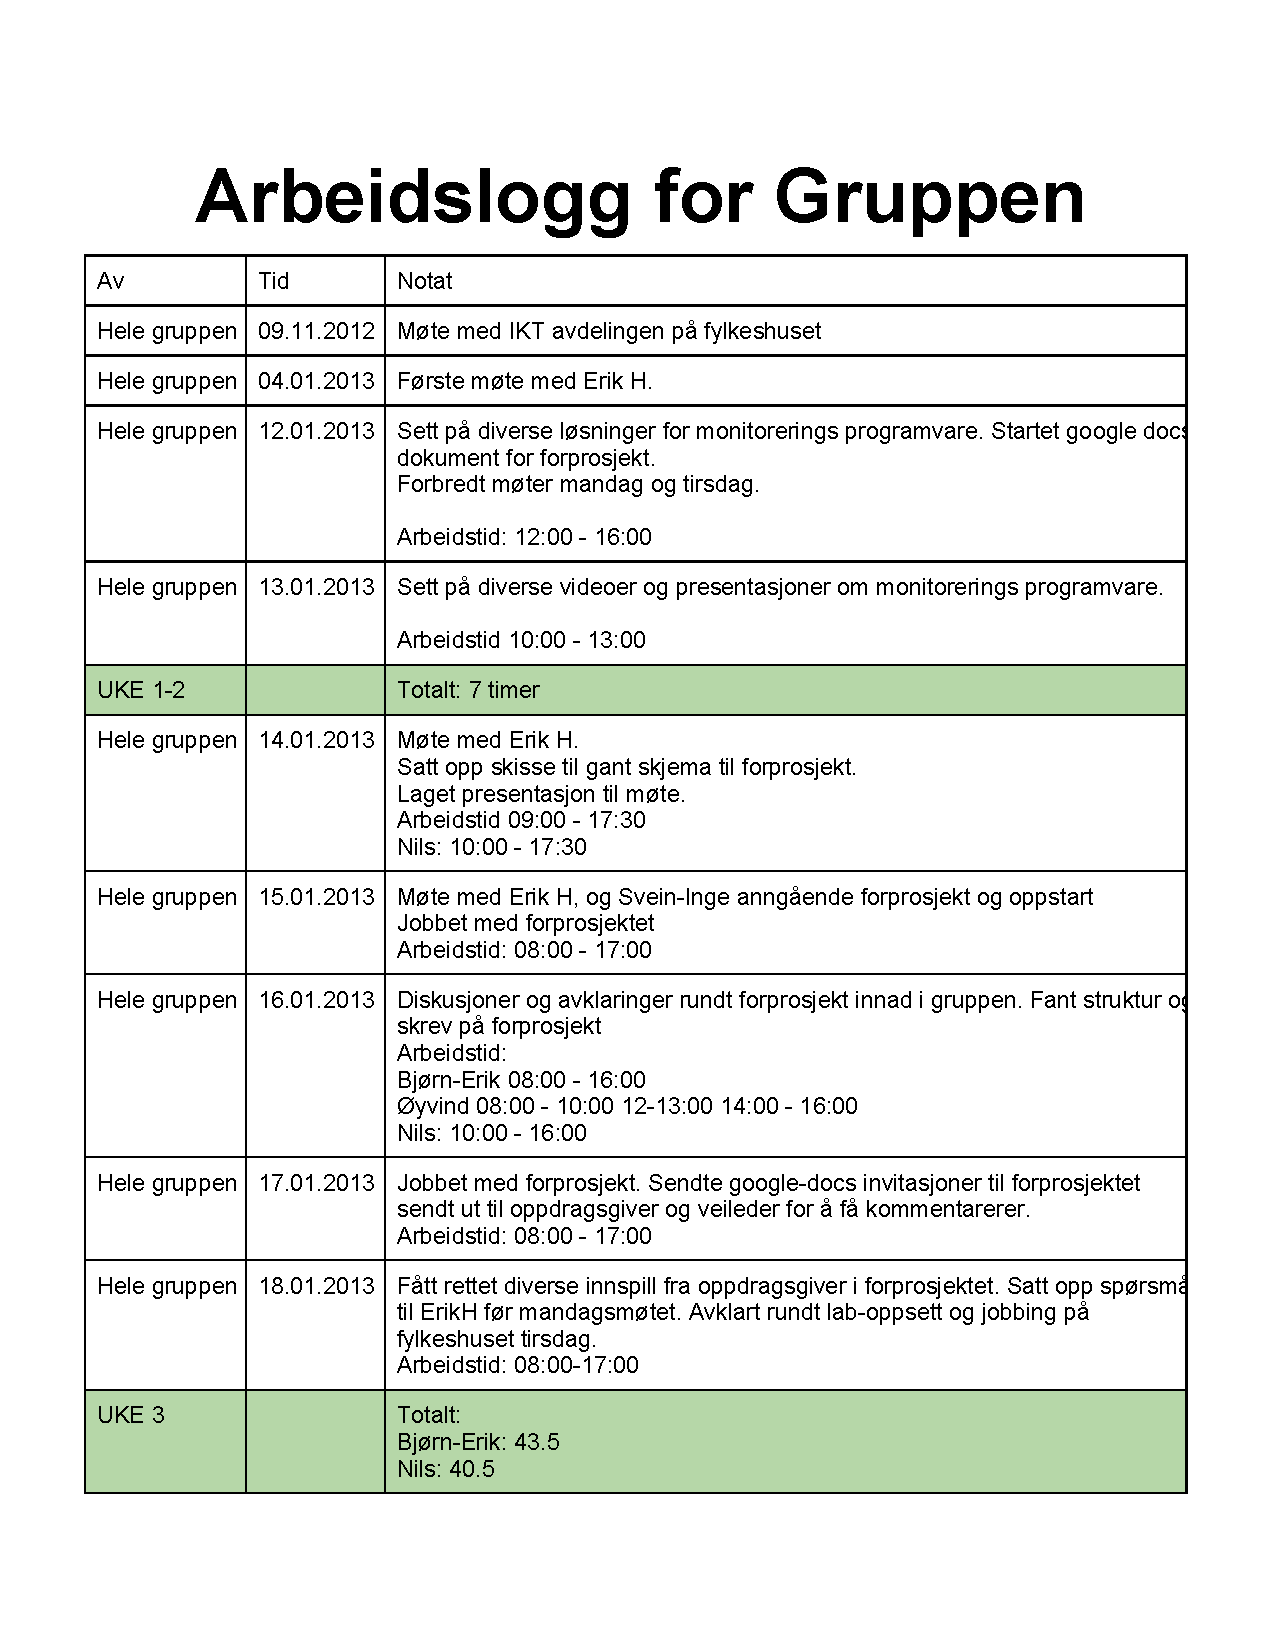
\includepdf[pages=-]{vedlegg/GruppeLogg.pdf}

\chapter{Møtereferater}\label{app:motereferat}
I dette vedlegget ligger møtereferater fra prosjektperioden.
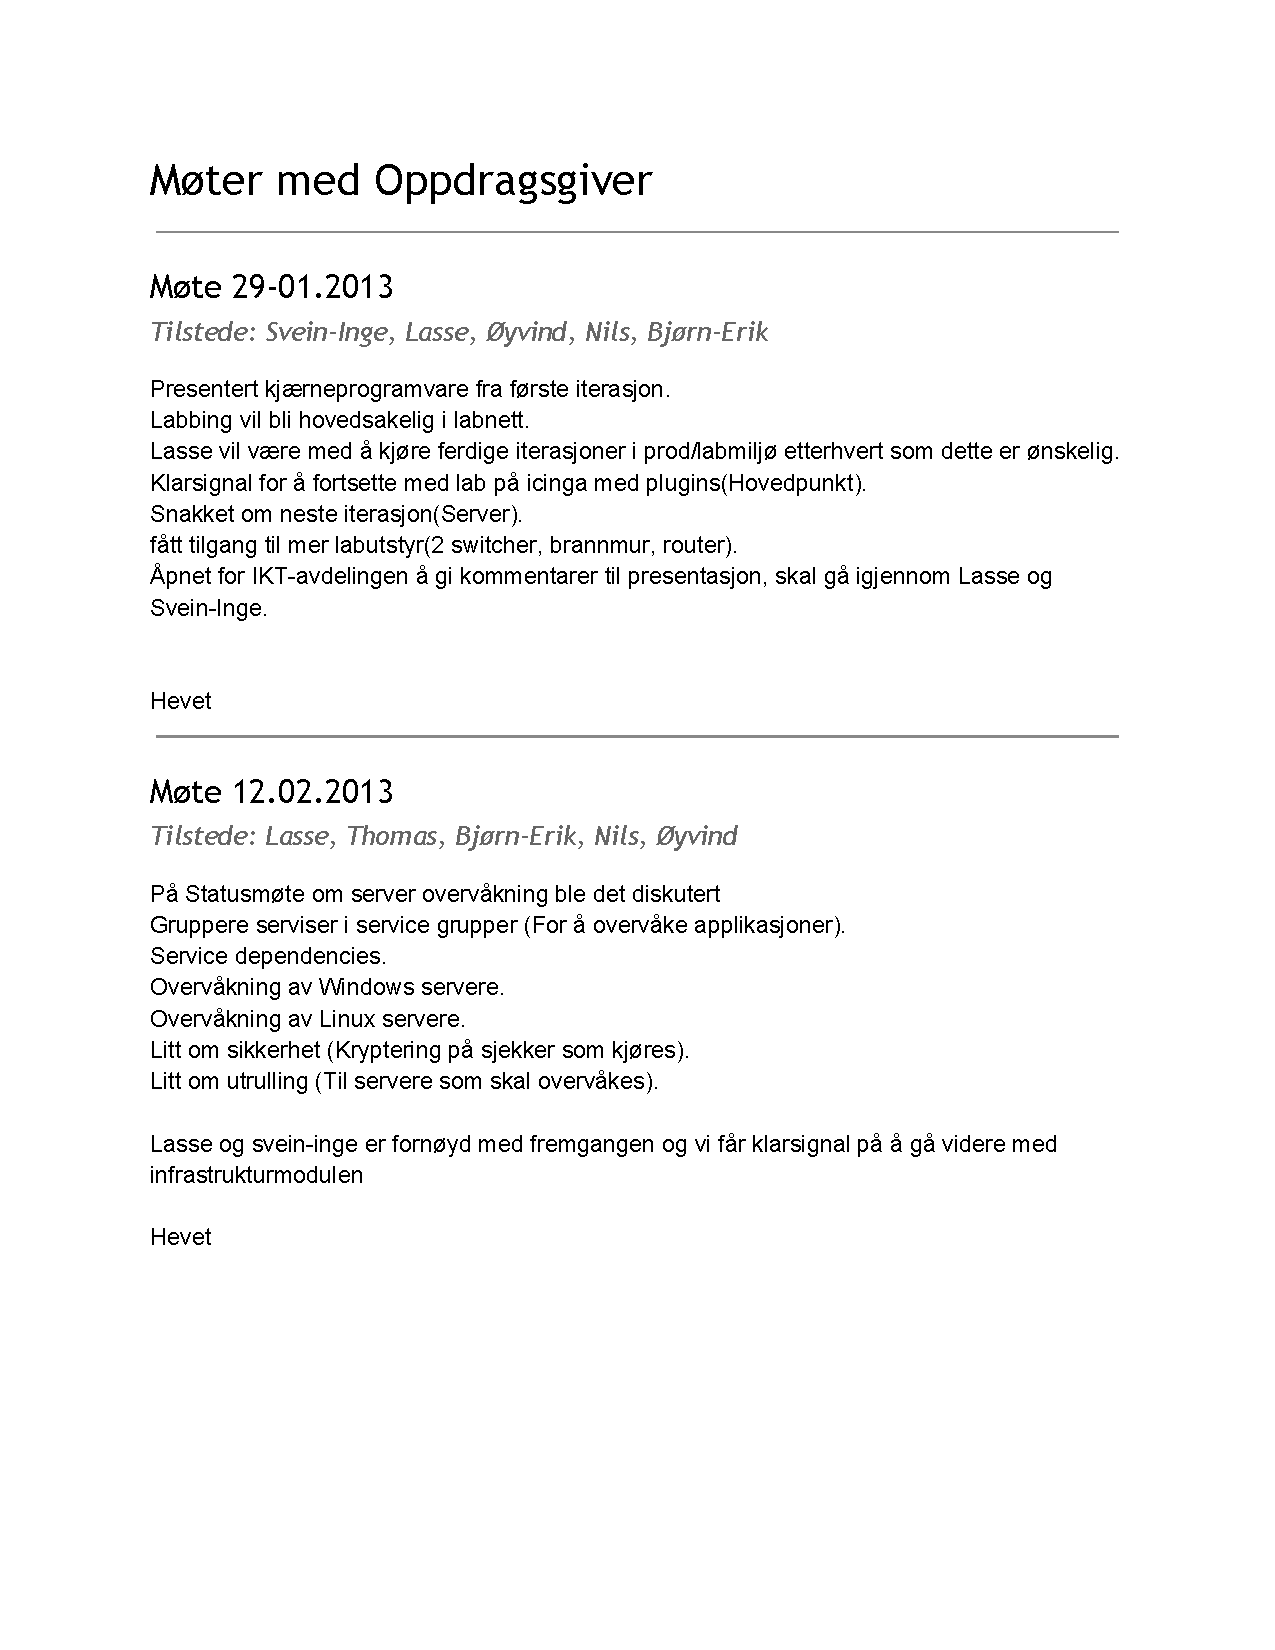
\includepdf[pages=-]{vedlegg/moteref.pdf}

\chapter{Presentasjoner}\label{app:presentasjoner}
I dette vedlegget ligger presentasjoner som har blitt holdt for IKT avdelingen gjennom prosjektet.

\includepdf[pages=-,landscape=true]{vedlegg/15_01_2013forprosjektmote.pdf}

\includepdf[pages=-,landscape=true]{vedlegg/29_01_2013Icinga.pdf}

\includepdf[pages=-,landscape=true]{vedlegg/05_03_2013ServerogInfrastruktur.pdf}

\chapter{Dokumenter}\label{app:dokumenter}
I dette vedlegget finnes:\\ 
\indent Kartlegging av behov, som ble laget av MonKey og utredet sammen med IKT-avdelingen.\\
\indent Opplæringsdokument som ble gjennomgått sammen med Oppdragsgiver og Teknisk kontakt ved slutten av prosjektperioden.
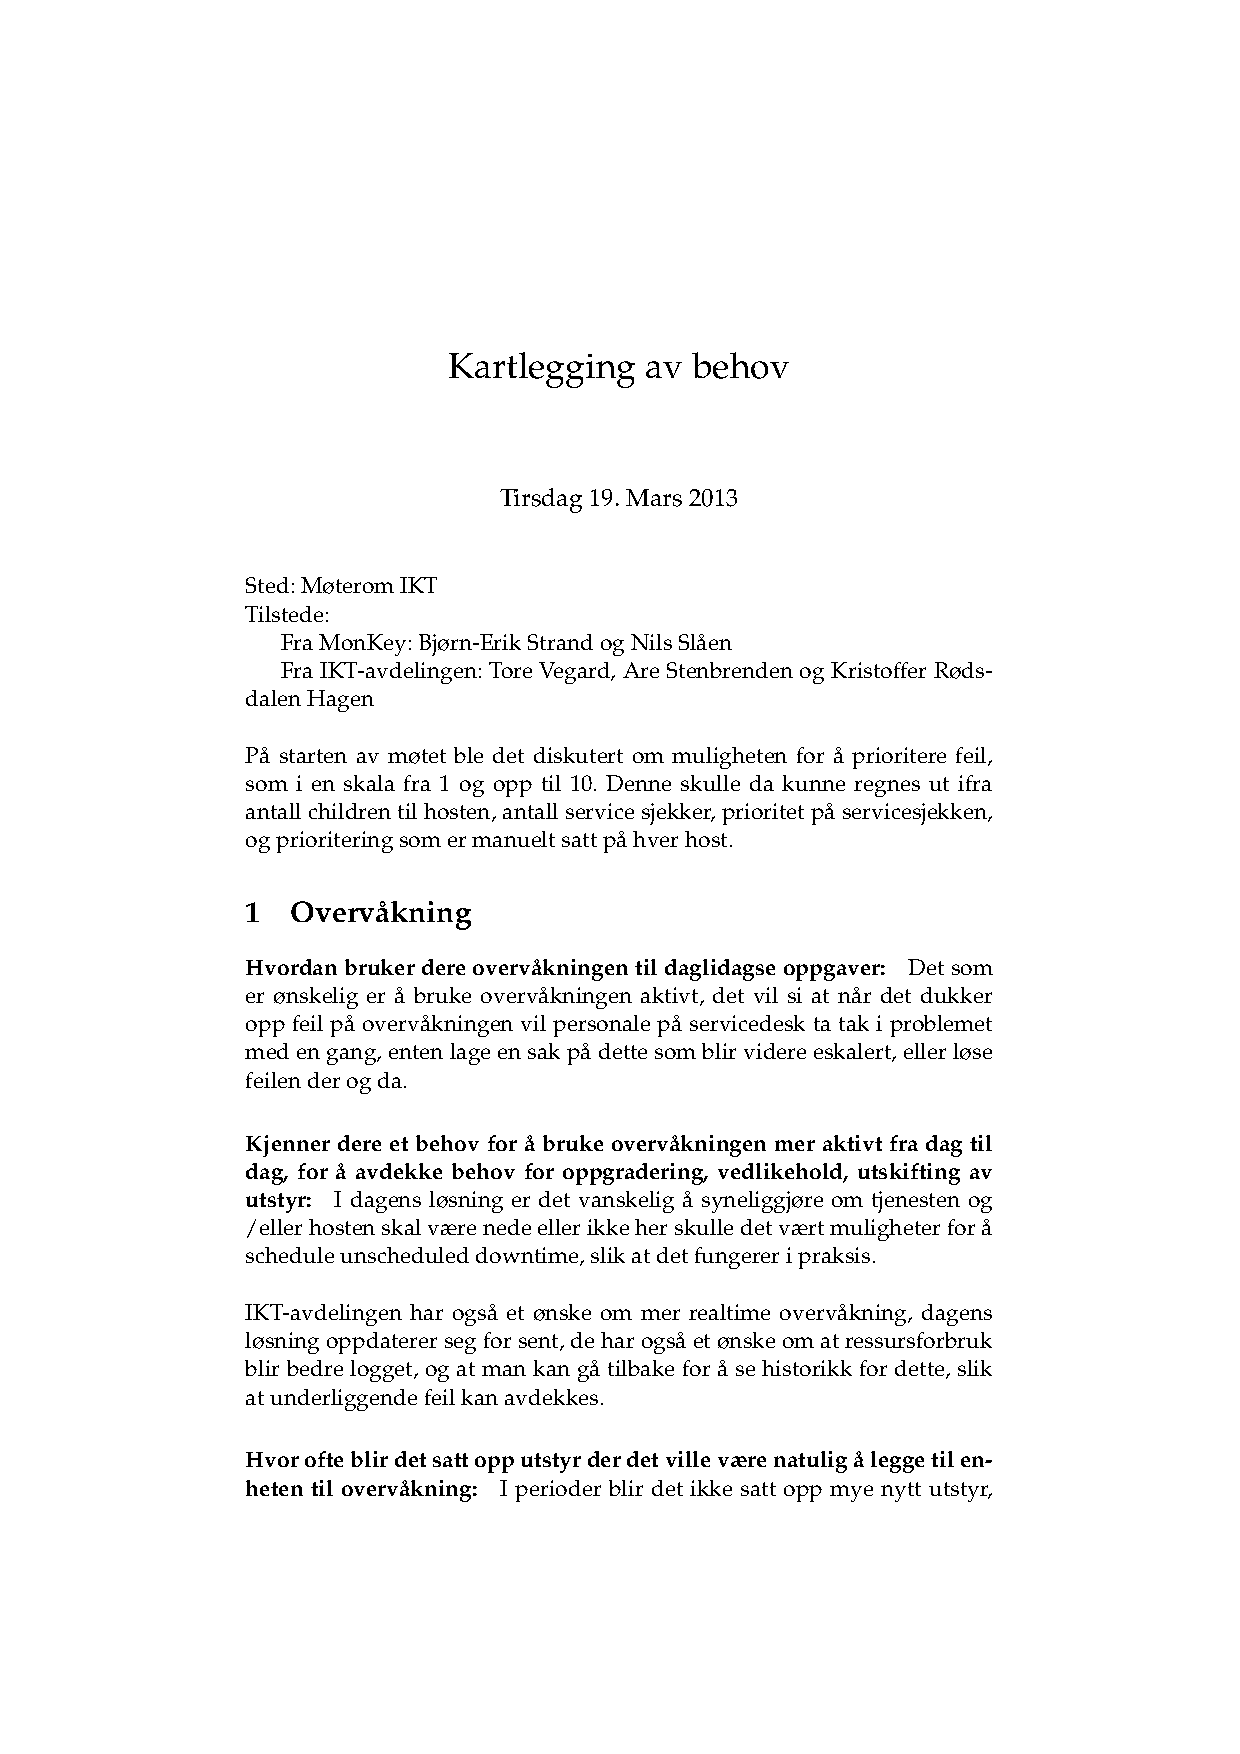
\includepdf[pages=-, pagecommand={\label{kartlegging}}]{vedlegg/kartlegging}
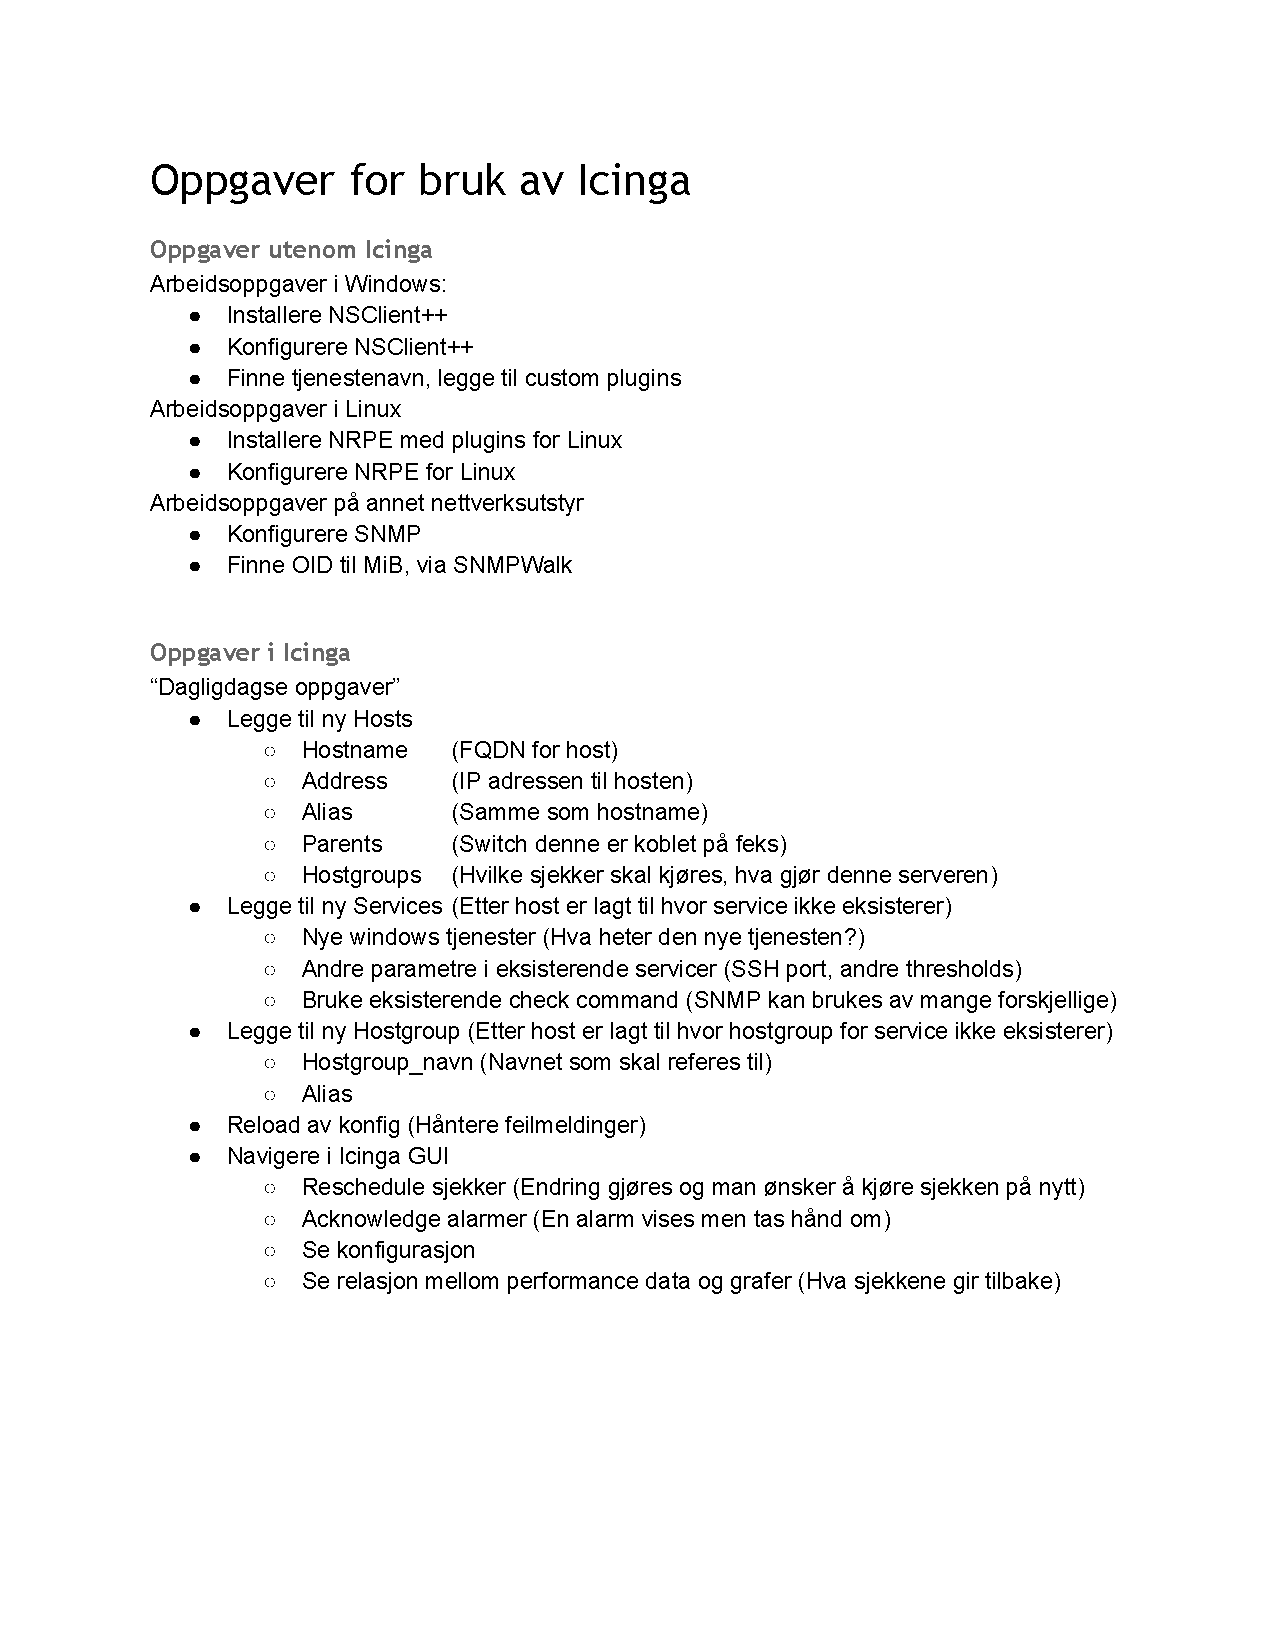
\includepdf[pages=-, pagecommand={\label{opplaering}}]{vedlegg/Opplaering}
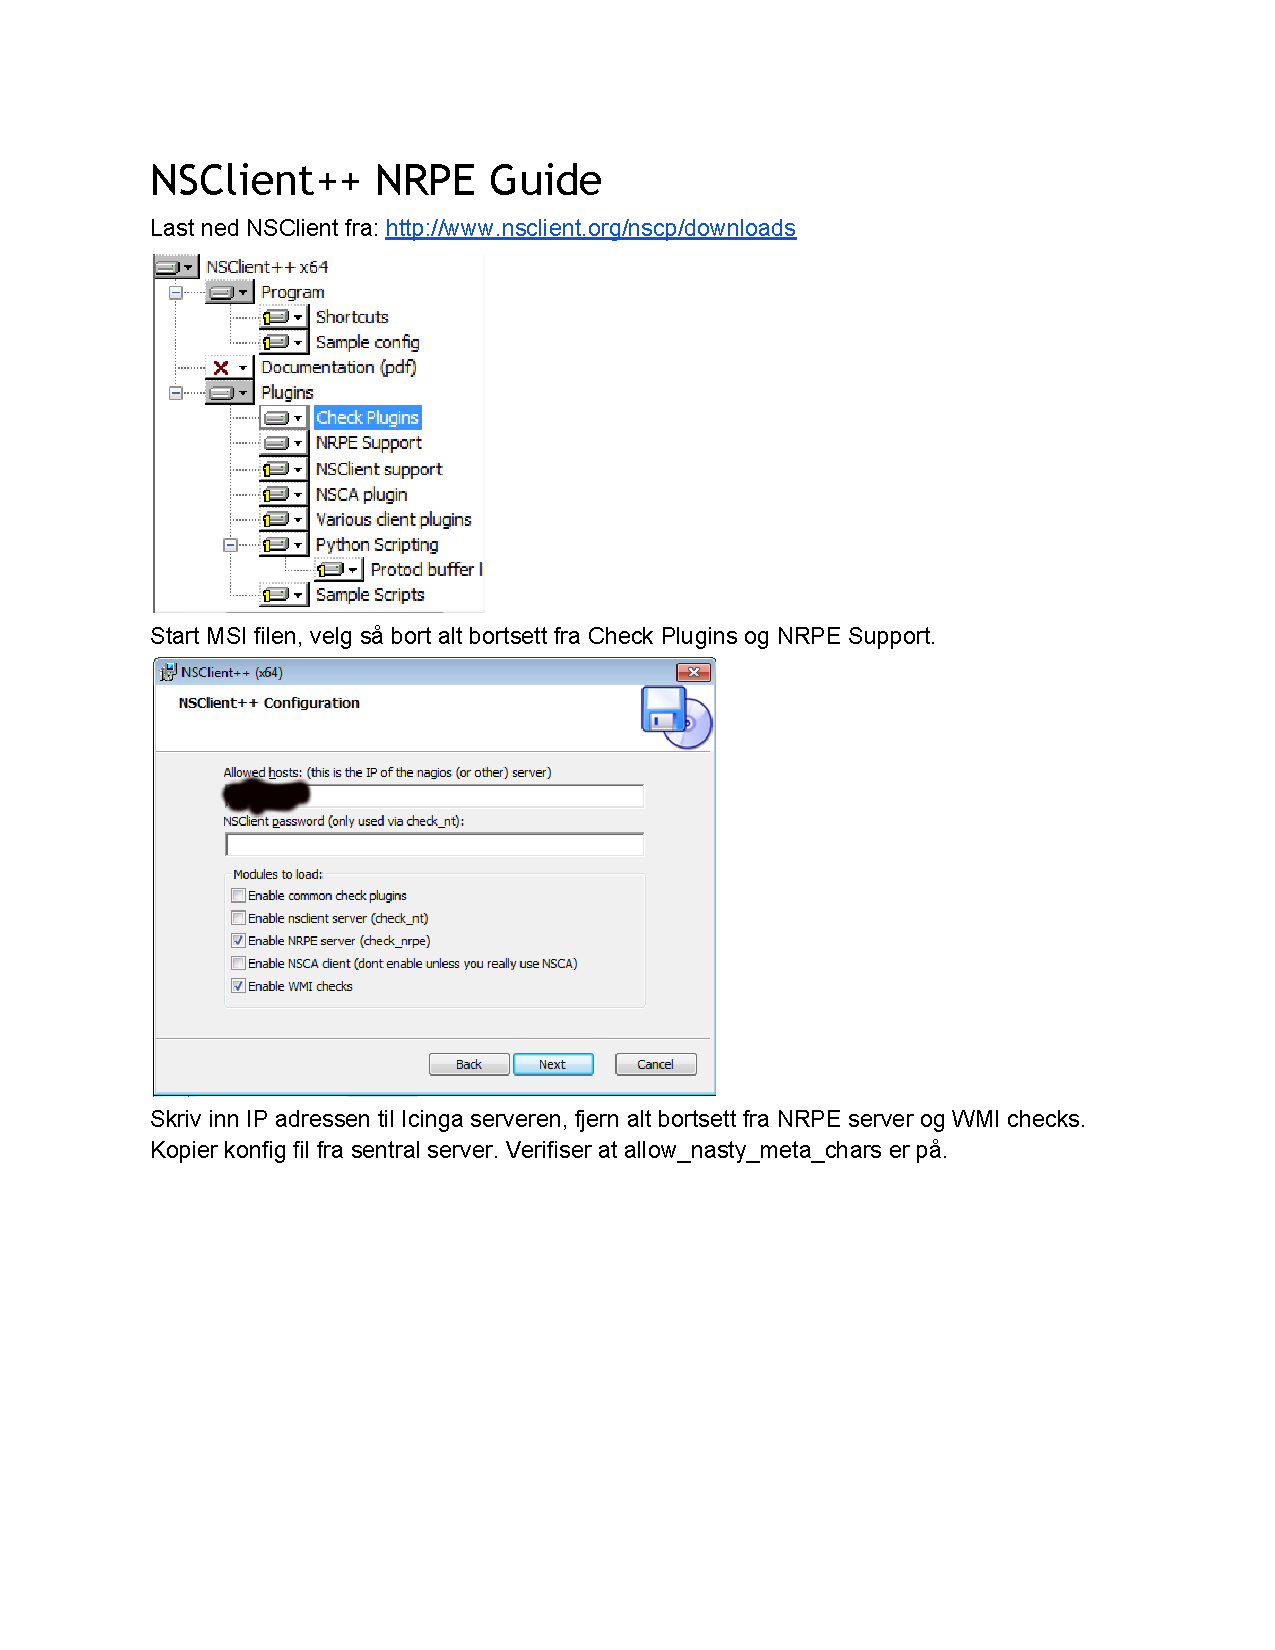
\includepdf[pages=-, pagecommand={\label{agentguide}}]{vedlegg/installagent.pdf}

\chapter{Statusrapporter}\label{app:statusrapporter}
I dette vedlegget finnes statusrapporter skrevet for hver iterasjon.
%\modifiedincludepdf{-}{status2}{status/status2.pdf}

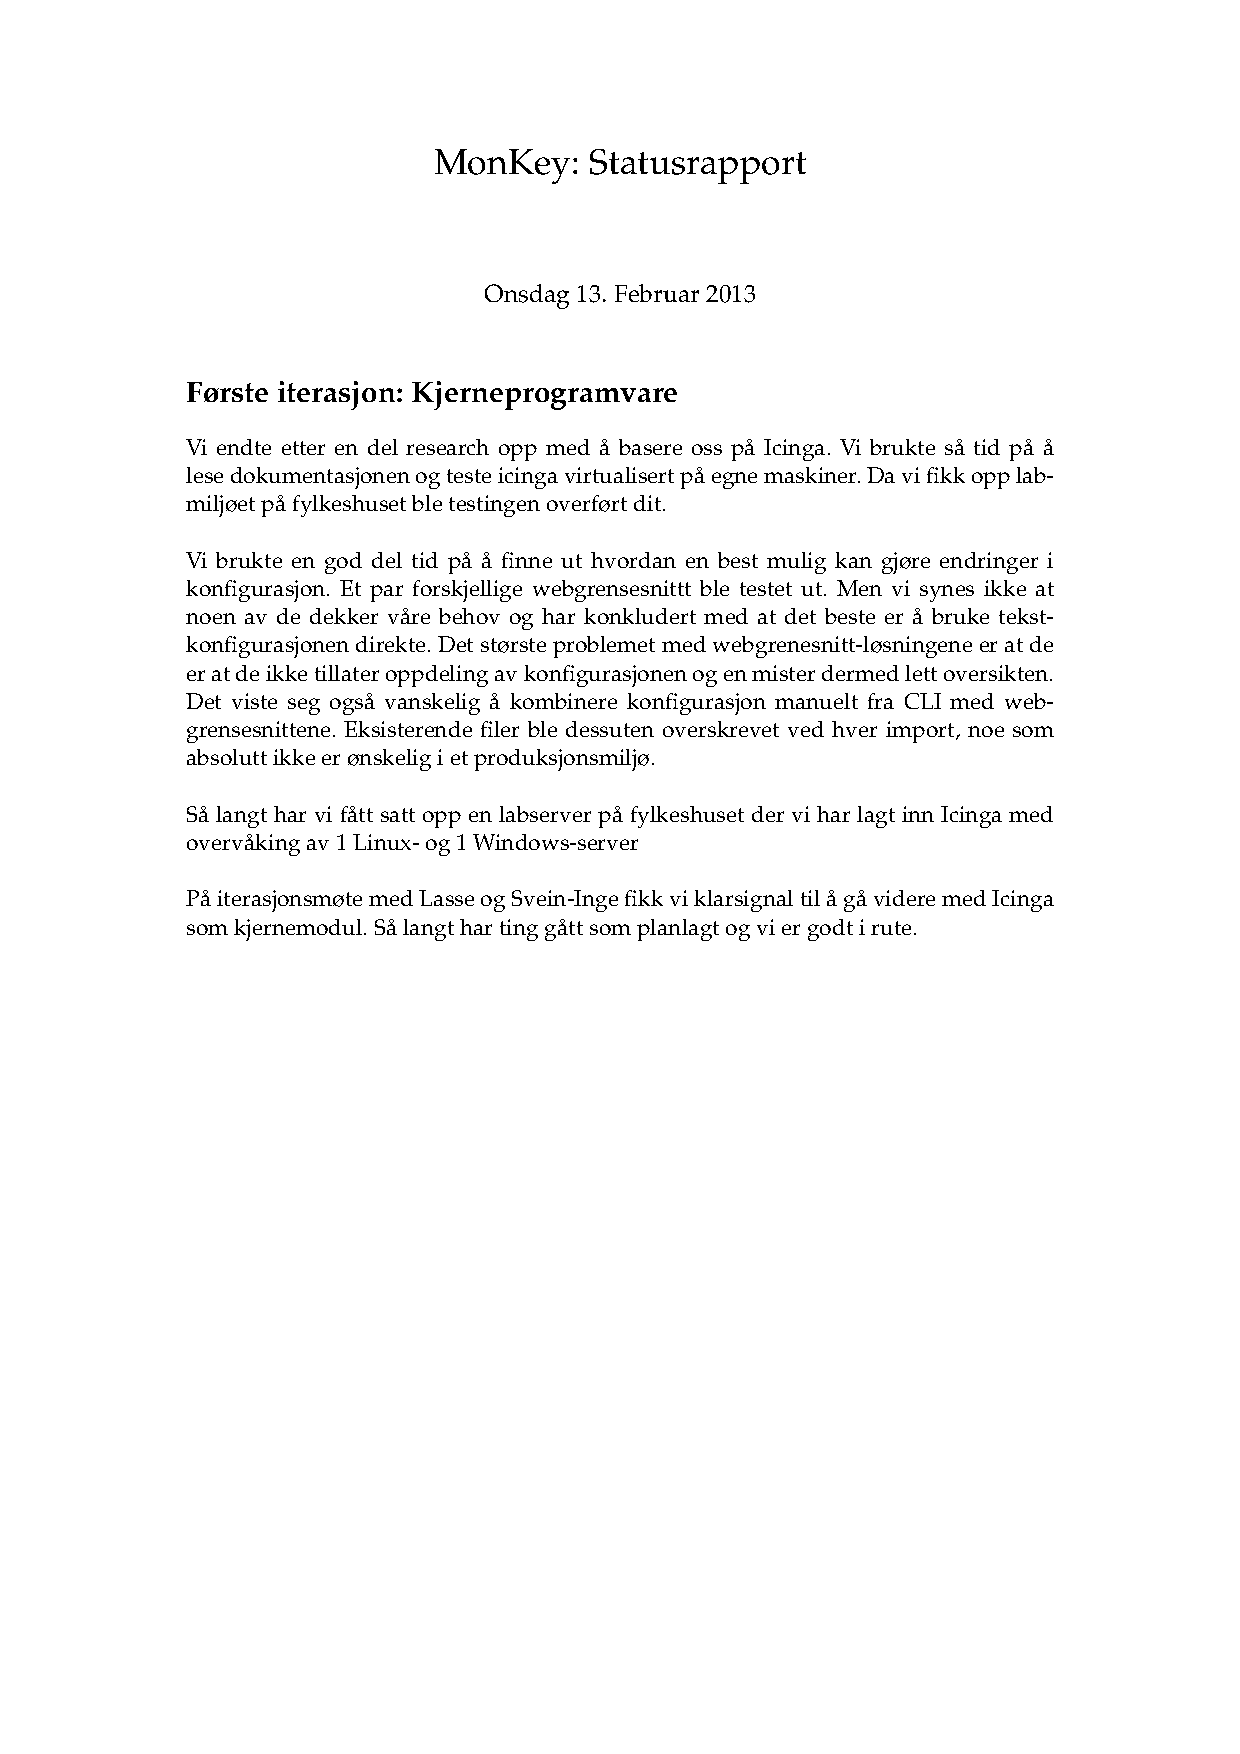
\includepdf[pages=-]{status/status1.pdf}
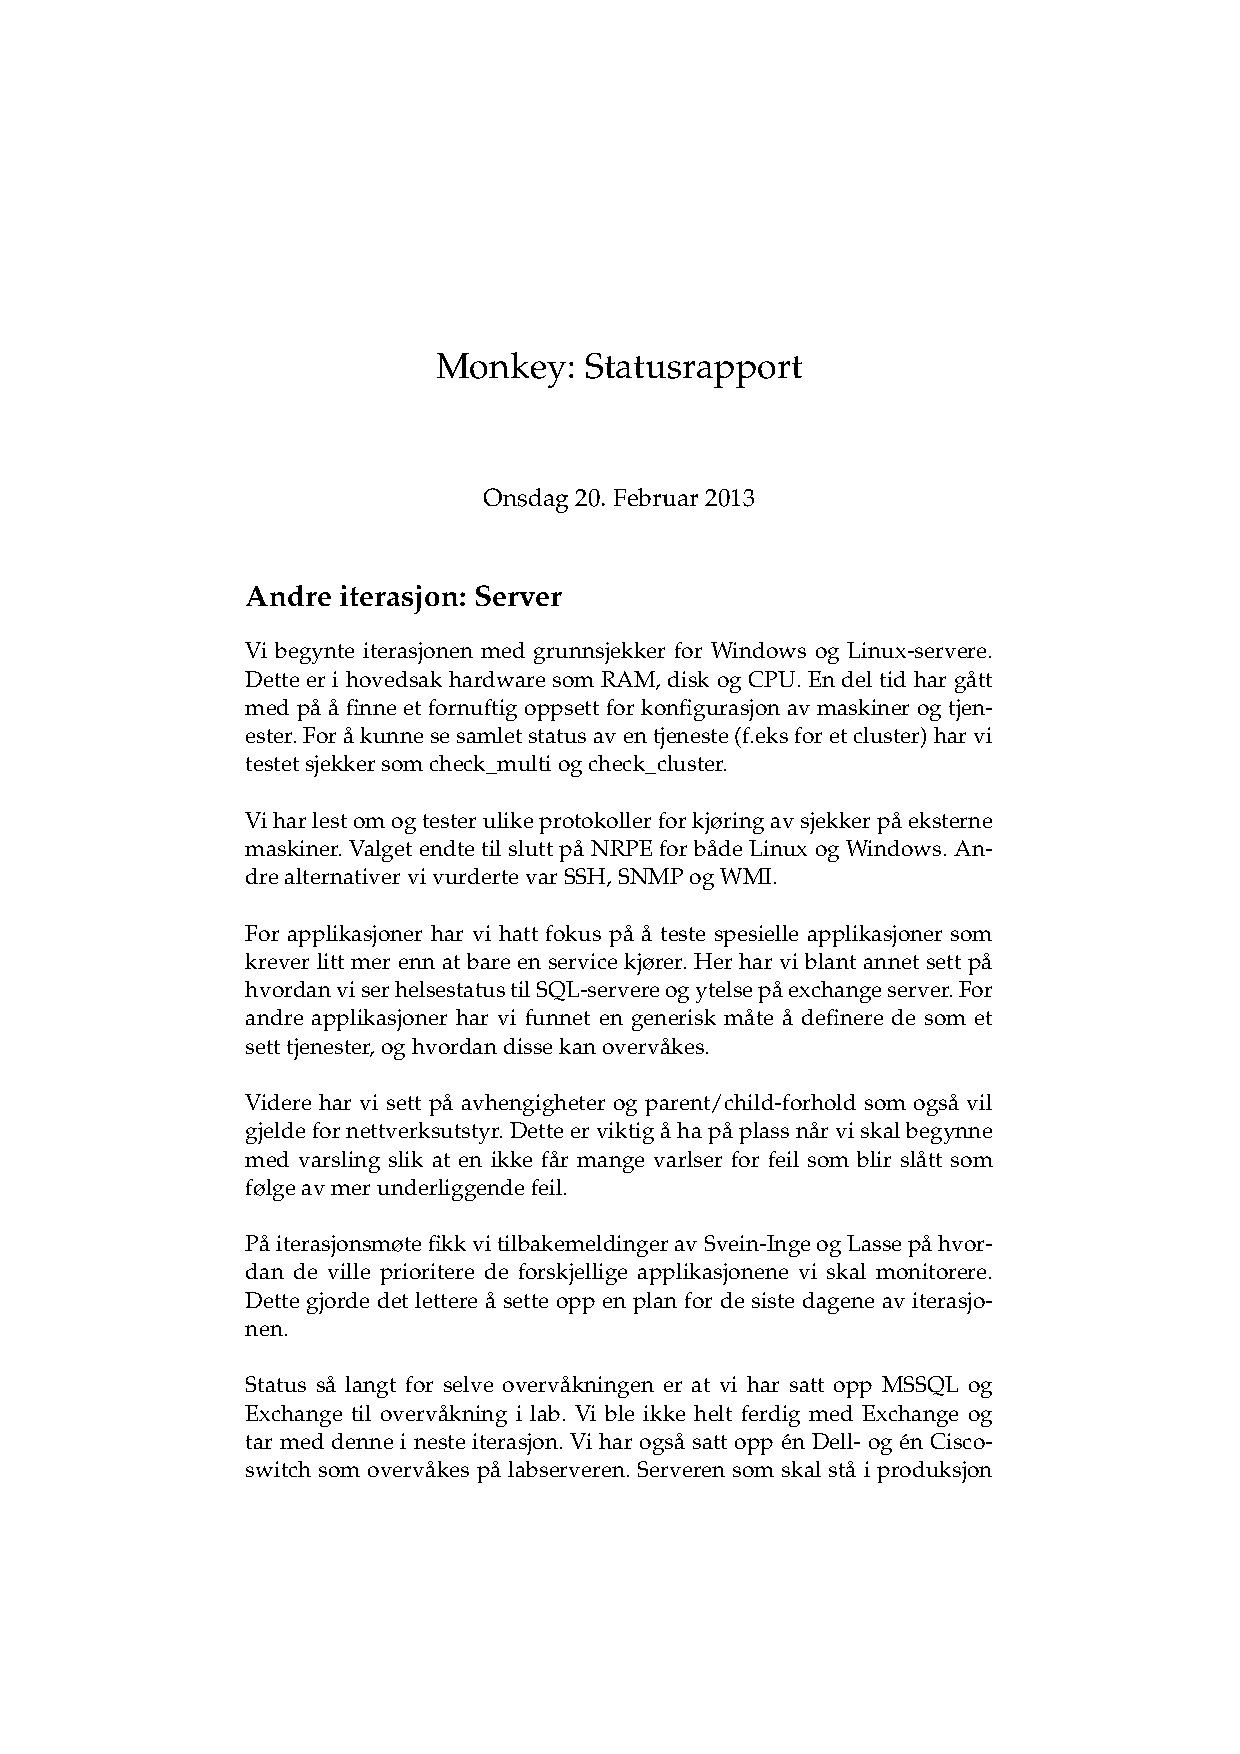
\includepdf[pages=-]{status/status2.pdf}
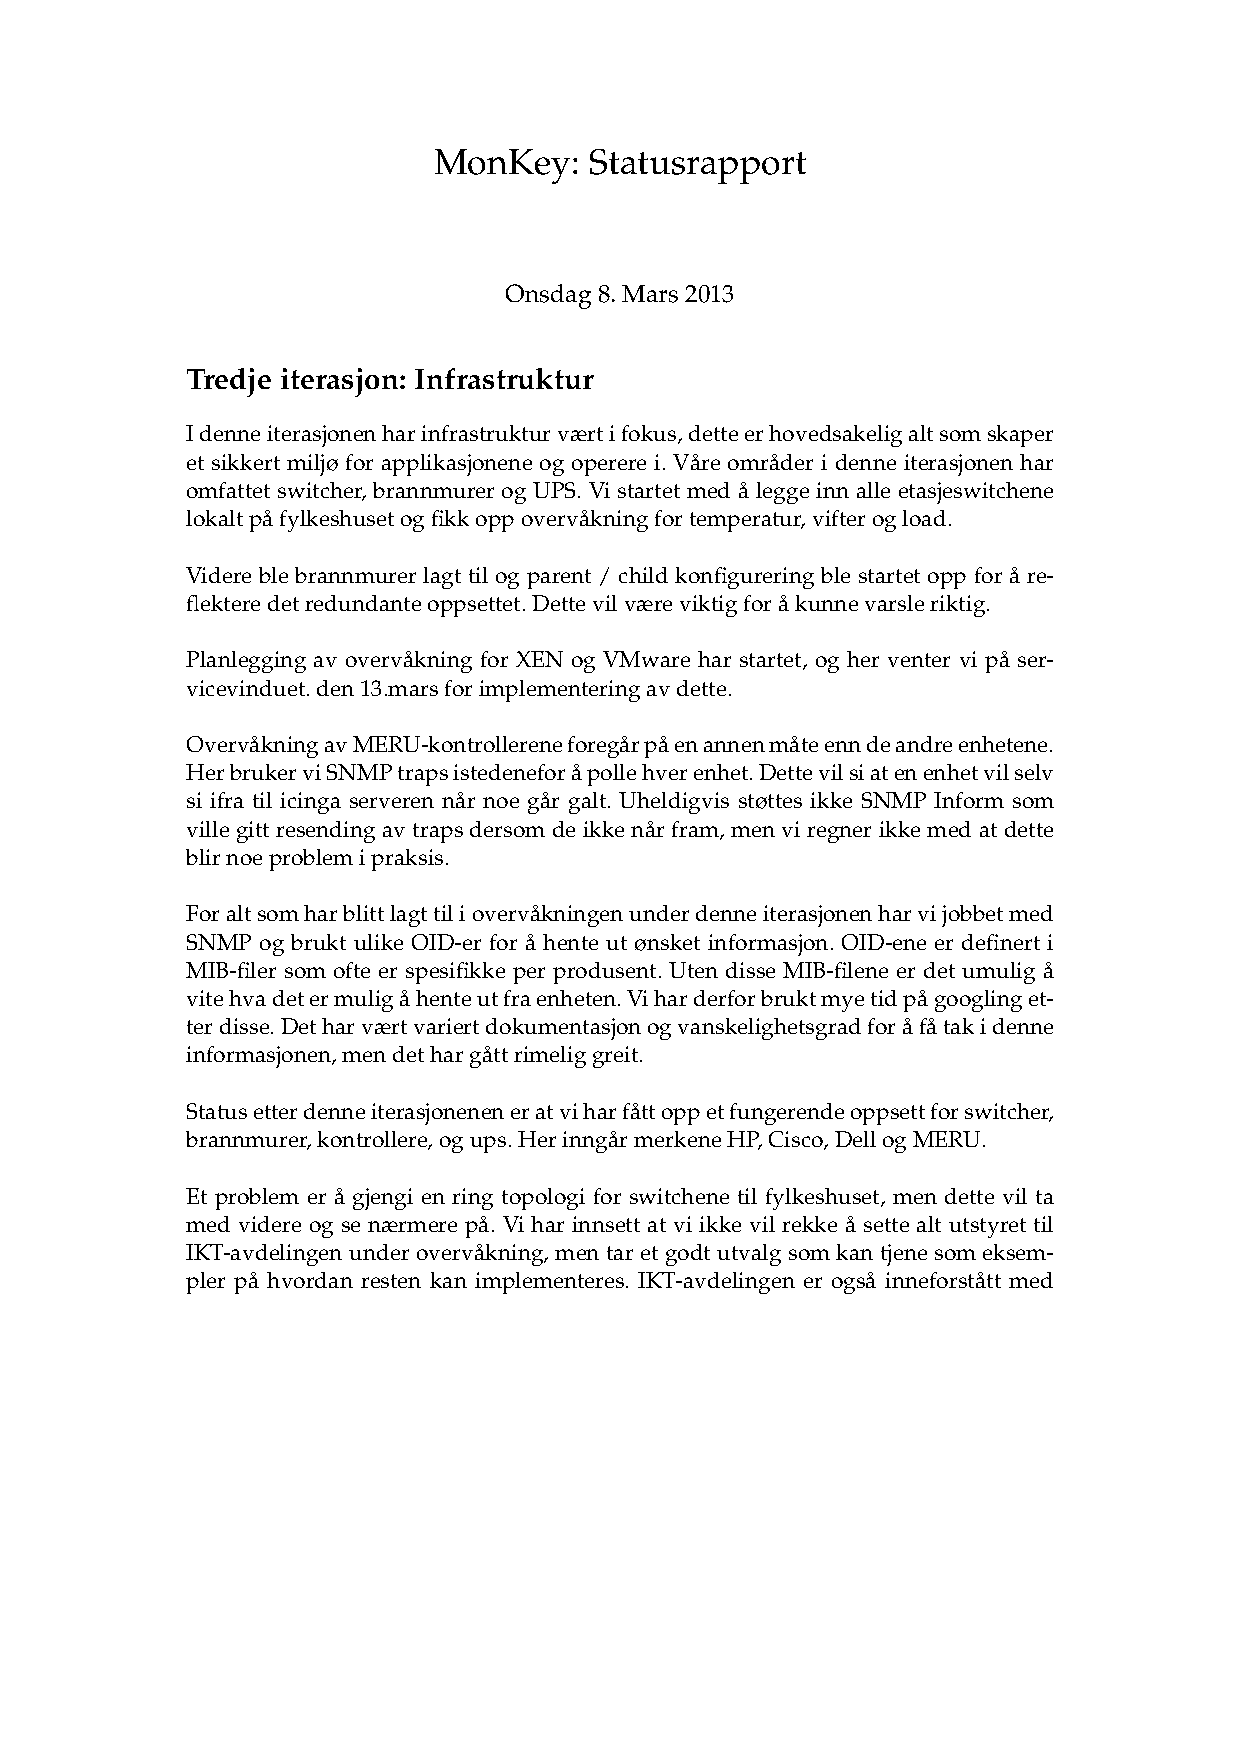
\includepdf[pages=-]{status/status3.pdf}
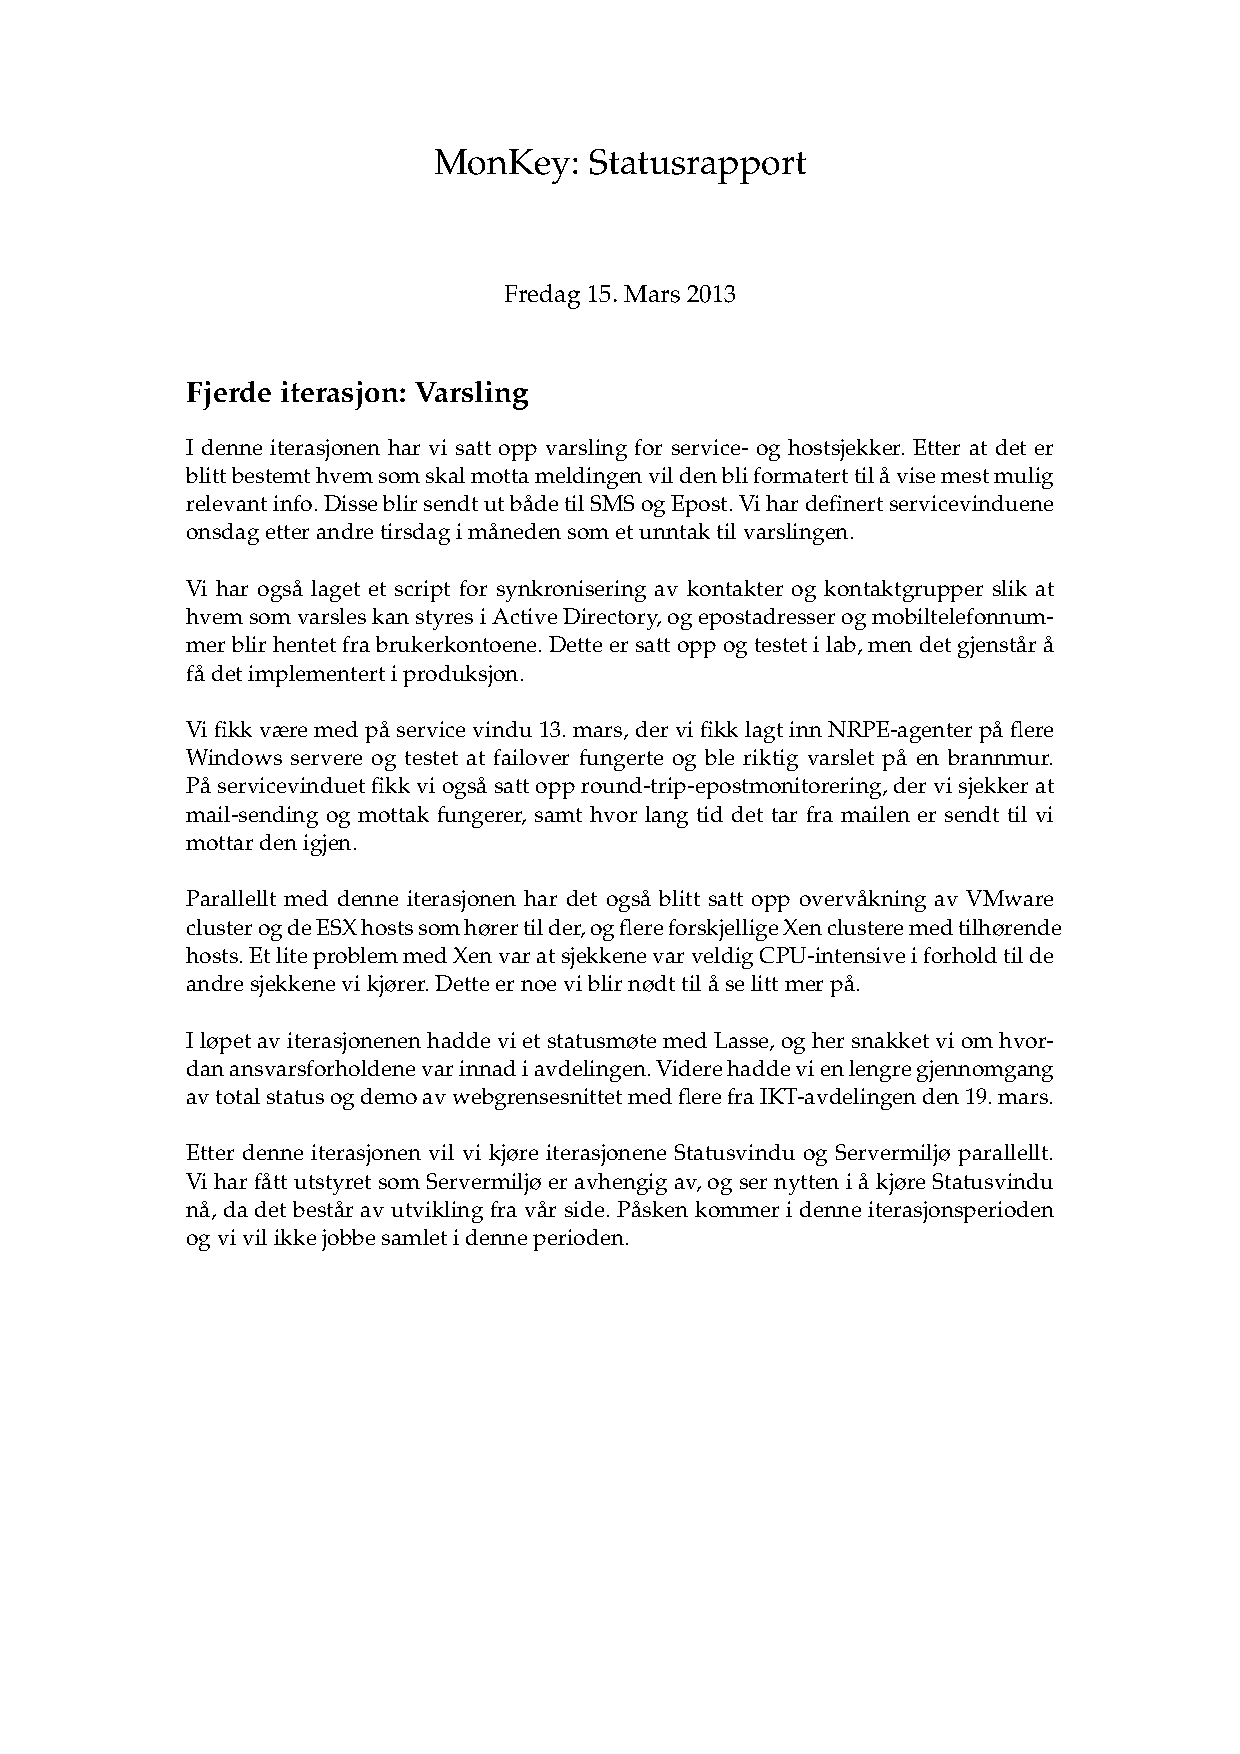
\includepdf[pages=-]{status/status4.pdf}

\includepdf[pages=-]{status/status5.pdf}
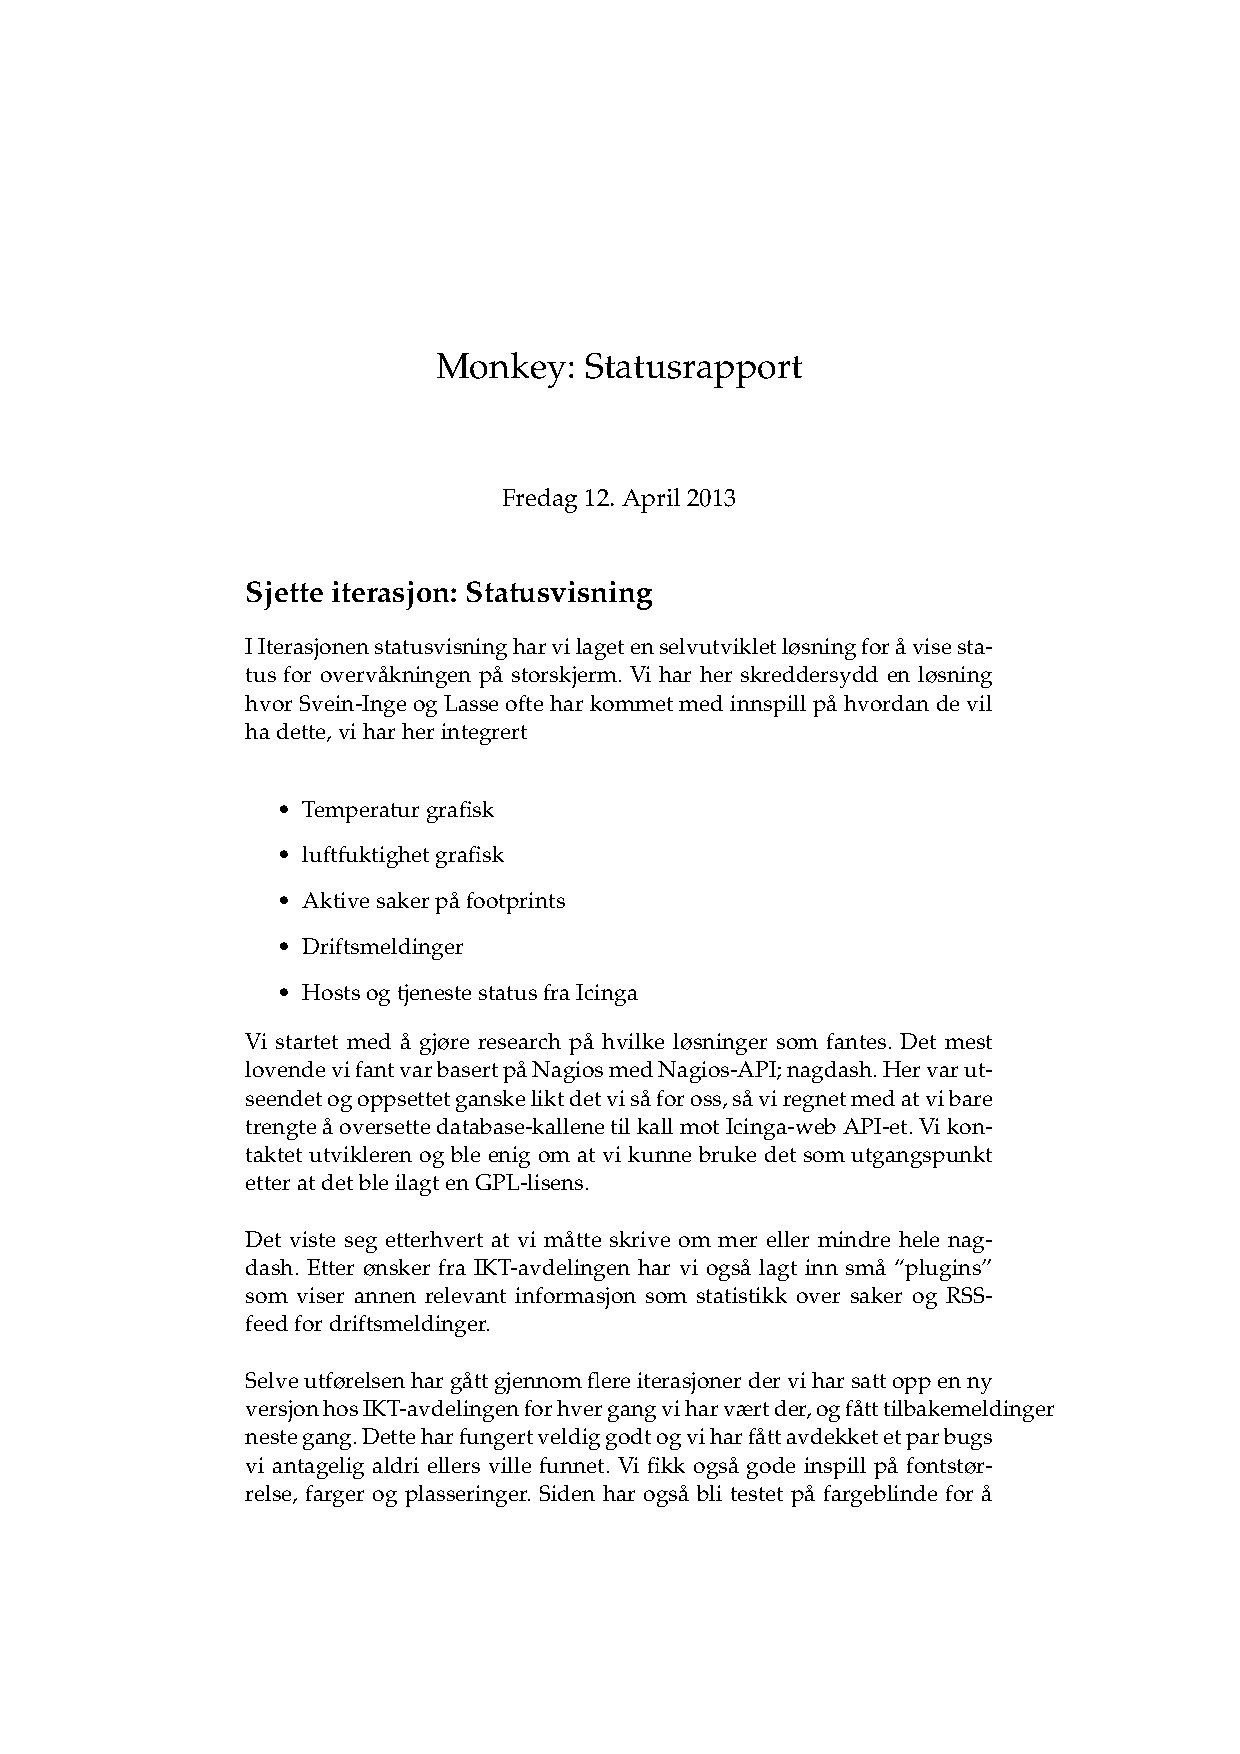
\includepdf[pages=-]{status/status6.pdf}

\chapter{Forprosjekt}\label{app:forprosjekt}
I dette vedlegget finnes forprosjektet for MonKey
%\modifiedincludepdf{-}{forprosjekt}{forprosjekt.pdf}

\includepdf[pages=-]{forprosjekt.pdf}

\chapter{Kildekode}\label{app:kildekode}
Selvskrevene kildekode er lagt ved under dette vedlegget. Innholder plugins og generering av host-er script.

\begin{changemargin}{-1cm}{-1cm}
\section{Host generering}
\lstinputlisting[language=Bash, label={gen.bash}]{script/gen.bash}

\section{Active Directory Kontakt Sync}
\lstinputlisting[language=Perl, label={ad_sync.pl}]{script/ad_sync.pl}

\section{Check NDB Mem}
\lstinputlisting[language=Perl, label={check_ndb_mem.pl}]{script/check_ndb_mem.pl}
\clearpage
\section{SQL Brukeroppretting}
\lstinputlisting[language=sql, label={oracledb.sql}]{script/oracledb.sql}
\lstinputlisting[language=sql, label={mssqldb.sql}]{script/mssqldb.sql}
\section{Init-script}
\lstinputlisting[language=Bash, label={metricinga_init.d}]{script/metricinga_init.d}

\section{Statusvindu Kildekode}
\lstinputlisting[language=PHP, label={index.php}]{script/index.php}
\lstinputlisting[language=PHP, label={nagdash.php}]{script/nagdash.php}
\lstinputlisting[language=PHP, label={netbotz.php}]{script/netbotz.php}
\lstinputlisting[language=PHP, label={rss.php}]{script/rss.php}
\lstinputlisting[language=PHP, label={image.php}]{script/image.php}
\lstinputlisting[language=PHP, label={footprints.php}]{script/footprints.php}
\lstinputlisting[language=PHP, label={config.php}]{script/config.php}
\lstinputlisting[language=PHP, label={db_config.php}]{script/db_config.php}
\lstinputlisting[language=PHP, label={external.js}]{script/external.js}
\clearpage
\lstinputlisting[language=HTML, label={style.css}]{script/style.css}
\clearpage
\section{Differanse på nedlastede plug-ins}
\inputencoding{latin1}
\lstinputlisting[label={diff.pl}]{vedlegg/diff.pl}
\end{changemargin}

\chapter{Epost}\label{epost}
Eposter av relevans for rapporten, svar er fjernet av hensyn til mottaker.
\clearpage
\verbatiminput{vedlegg/customvariable_mail.txt}
\noindent\rule{\textwidth}{0.4pt}
\verbatiminput{vedlegg/nagdashauthor_mail.txt}
\noindent\rule{\textwidth}{0.4pt}
\verbatiminput{vedlegg/hwgroup_mail.txt}
\clearpage
\verbatiminput{vedlegg/wathergoose_mail.txt}
\noindent\rule{\textwidth}{0.4pt}
\verbatiminput{vedlegg/database_mail.txt}\label{app:maildb}
\clearpage
\verbatiminput{vedlegg/servermiljo_mail.txt}
\clearpage
\verbinput{vedlegg/check_xenapi_mail.txt}
\end{appendices}

\end{document}
